%% using template from bare_conf.tex V1.3 2007/01/11
%% by Michael Shell
%% See:
%% http://www.michaelshell.org/
%% for current contact information.
%
%\documentclass[10pt, a4paper, onecolumn]{../IEEEtran}
%\documentclass[12pt, a4paper, twoside]{report}
\documentclass[12pt, a4paper, oneside]{report}
\usepackage[utf8]{inputenc}
\usepackage{datetime}

% \usepackage{cite}
% http://www.ctan.org/tex-archive/macros/latex/contrib/cite/
% The documentation is contained in the cite.sty file itself.
\usepackage[final]{pdfpages}


\usepackage[american]{babel}
\usepackage{csquotes}
% http://ftp.cc.uoc.gr/mirrors/CTAN/macros/latex/contrib/biblatex-contrib/biblatex-apa/biblatex-apa.pdf
\usepackage[style=apa,natbib=true]{biblatex}
% \usepackage[style=ieee,natbib=true]{biblatex}

% \bibliographystyle{apalike}
% \newcommand{\autocity}[1]{\ref{#1}}

% References to be like APA recommendations
\usepackage{apalike}
% in case of conflict might use the line below
% \let\bibhang\relax

\DeclareLanguageMapping{american}{american-apa}

% trials
%\DeclareFieldFormat{titlecase}{\MakeSentenceCase{#1}}
%\DeclareFieldFormat{titlecase}{#1}
%\DeclareFieldFormat{journaltitle}{\MakeCapital{\mkbibemph{#1}}XYZ,} % italic journal title with comma
%\DeclareFieldFormat[inbook,thesis]{title}{\MakeCapital{\mkbibemph{#1}}XXX\addperiod} % italic title with period
%\DeclareFieldFormat[article]{title}{#1} % title of journal article is printed as normal text


\bibliography{ref}


\usepackage{fontspec}
\setmainfont{Times New Roman}

% per script fonts
% \usepackage{polyglossia}
% \setmainlanguage{english}
% \setotherlanguage{arabic}
% [Script=Latin, Scale=1]{Times New Roman}
% [Script=Arabic, Scale=1]{Droid Sans}

% \usepackage[pass]{geometry} 
% \geometry{a4paper,left=35mm,right=25mm,top=25mm,bottom=25mm,}
\usepackage[a4paper,left=25mm,right=25mm,top=25mm,bottom=25mm,bindingoffset=10mm]{geometry}

% Indent first paragraph in each section
\usepackage{indentfirst}

% Format the titles and sections, psut style
\usepackage{titlesec}

\titlespacing*{\chapter}{-1.5mm}{2ex}{1ex}
\titlespacing*{\section}{0pt}{2ex}{1ex}
\titlespacing*{\subsection}{0pt}{2ex}{1ex}

\titleformat*{\section}{\fontsize{14pt}{1em}\selectfont\bfseries}
\titleformat*{\subsection}{\fontsize{14pt}{1em}\selectfont\bfseries}

\titleformat{\chapter}{
    \normalfont\bfseries}{
    % Format like "Chapter 1. Name of the Chapter"
    \fontsize{14pt}{1em}\selectfont \chaptertitlename \ \thechapter.
}{ % Remove uneeded line above the chapter
    0pt
}{ % The title format
    \fontsize{14pt}{1em}\selectfont
}

\usepackage[normalem]{ulem}
\useunder{\uline}{\ul}{}

% 1.5 line spacing
\usepackage{setspace}
\onehalfspacing

% psut paragraph style
\setlength{\parskip}{1em}



% Registered trademark sign
\usepackage{textcomp}



\usepackage{graphicx}
\graphicspath{{./figs/}}
\DeclareGraphicsExtensions{.pdf,.jpg,.jpeg,.png}
% http://www.ctan.org/tex-archive/macros/latex/required/graphics/

% \usepackage{subfig}
\usepackage[singlelinecheck=false]{caption}
\usepackage{subcaption}
\usepackage{wrapfig}
\usepackage{afterpage}
\usepackage{pdflscape}

\usepackage{rotating}

% *** MATH PACKAGES ***
% Allow multi-line math equations
\usepackage{amsthm}
\usepackage[cmex10]{amsmath}
\usepackage{amsfonts}
% http://www.ctan.org/tex-archive/macros/latex/required/amslatex/math/

\theoremstyle{definition}
\newtheorem{definition}{Definition}[section]

% *** SPECIALIZED LIST PACKAGES ***
%
%\usepackage{algorithmic}
% http://www.ctan.org/tex-archive/macros/latex/contrib/algorithms/
% algorithmicx.sty package by Szasz Janos:
% http://www.ctan.org/tex-archive/macros/latex/contrib/algorithmicx/

% *** ALIGNMENT PACKAGES ***
%
\usepackage{array}
% http://www.ctan.org/tex-archive/macros/latex/required/tools/
\usepackage{multirow,tabularx}
\usepackage{tabularx}           % Customized table formatting
\usepackage{environ}            % Used to define custom table environment
\usepackage{booktabs}
\usepackage{makecell}

% to be able to do \adjustwidth
% https://ctan.org/pkg/changepage
\usepackage{changepage}
\usepackage{framed}
\usepackage{mdframed}

%\usepackage{mdwmath}
%\usepackage{mdwtab}
% http://www.ctan.org/tex-archive/macros/latex/contrib/mdwtools/

%\usepackage{eqparbox}
% http://www.ctan.org/tex-archive/macros/latex/contrib/eqparbox/

% *** SUBFIGURE PACKAGES ***
%\usepackage[tight,footnotesize]{subfigure}
% http://www.ctan.org/tex-archive/obsolete/macros/latex/contrib/subfigure/

%\usepackage[caption=false]{caption}
%\usepackage[font=footnotesize]{subfig}
%\usepackage[caption=false,font=footnotesize]{subfig}
% http://www.ctan.org/tex-archive/macros/latex/contrib/subfig/
% http://www.ctan.org/tex-archive/macros/latex/contrib/caption/

\usepackage{aliascnt}
\usepackage{float}
\newaliascnt{eqfloat}{equation}
\newfloat{eqfloat}{h}{eqflts}
\floatname{eqfloat}{Equation}

\newcommand*{\ORGeqfloat}{}
\let\ORGeqfloat\eqfloat
\def\eqfloat{%
  \let\ORIGINALcaption\caption
  \def\caption{%
    \addtocounter{equation}{-1}%
    \ORIGINALcaption
  }%
  \ORGeqfloat
}

\floatstyle{ruled}
\newfloat{program}{thp}{lop}[section]
\floatname{program}{Program}

% *** FLOAT PACKAGES ***
%
%\usepackage{fixltx2e}
% http://www.ctan.org/tex-archive/macros/latex/base/

%\usepackage{stfloats}
% http://www.ctan.org/tex-archive/macros/latex/contrib/sttools/

% *** PDF, URL AND HYPERLINK PACKAGES ***
% http://ftp.cc.uoc.gr/mirrors/CTAN/macros/latex/contrib/hyperref/doc/manual.html#x1-90003.5
\usepackage[bookmarks,colorlinks=true,urlcolor=blue,linkcolor=black,citecolor=black]{hyperref}


% \usepackage{url}
% url.sty was written by Donald Arseneau. It provides better support for
% handling and breaking URLs. url.sty is already installed on most LaTeX
% systems. The latest version can be obtained at:
% http://www.ctan.org/tex-archive/macros/latex/contrib/misc/
% Read the url.sty source comments for usage information. Basically,
% \url{my_url_here}.

% *** Do not adjust lengths that control margins, column widths, etc. ***
% *** Do not use packages that alter fonts (such as pslatex).         ***
% There should be no need to do such things with IEEEtran.cls V1.6 and later.
% (Unless specifically asked to do so by the journal or conference you plan
% to submit to, of course. )

% must be after \usepackage{hyperref}
\usepackage[acronym,toc]{glossaries}
\makenoidxglossaries
% \makeglossaries
\newacronym{ai}{AI}{Artificial Intelligence}
\newacronym{c2c}{C2C}{Customer to Customer}
\newacronym{ml}{ML}{Machine Learning}
\newacronym{ann}{ANN}{Artificial Neural Networks}
\newacronym{nn}{NN}{Neural Networks}
\newacronym{relu}{ReLU}{Rectified Linear Unit}
\newacronym{cnn}{CNN}{Convolutional Neural Network}
\newacronym{convnet}{ConvNet}{Convolutional Neural Network}
\newacronym{cifar}{CIFAR}{Canadian Institute for Advanced Research}
\newacronym{ilsvrc}{ILSVRC}{Large Scale Visual Recognition Challenge}
\newacronym{minst}{MINST}{Modified National Institute of Standards and Technology}
\newacronym{rnn}{RNN}{Recurrent Neural Network}
\newacronym{svm}{SVM}{Support Vector Machine}
\newacronym{sgd}{SGD}{Stochastic Gradient Descent}
\newacronym{cpu}{CPU}{Central Processing Unit}
\newacronym{gpu}{GPU}{Graphics Processing Unit}



% correct bad hyphenation here
\hyphenation{op-tical net-works semi-conduc-tor}

\title{Image recognition by knowledge transfer using deep convolutional neural network}
\author{Muayyad Saleh Alsadi \\ Princess Sumaya University for Technology}
\date{June, 2017}

\begin{document}

\begin{titlepage}
\singlespacing
\centering
\bfseries
\vspace{24pt}
{
\includegraphics[width=4.2cm]{psut_logo}\par}
\vspace{24pt}
{\fontsize{24pt}{36pt}\selectfont Using Deep Convolutional Neural Networks and Knowledge Transfer for Image Recognition \par}
\vspace{24pt}
{\fontsize{16pt}{24pt}\selectfont
By\\
Muayyad Alsadi\par}
\vspace{36pt}
{\fontsize{16pt}{24pt}\selectfont
Supervisor\\
Prof. Arafat Awajan\par}
\vspace{24pt}
{\fontsize{14pt}{21pt}\selectfont
Thesis Submitted in Partial Fulfillment of the Requirements for the
Degree of Master of Science in Computer Science\par}
\vspace{24pt}
{\fontsize{16pt}{24pt}\selectfont
Princess Sumaya University for Technology\\
King Abdullah I School of Graduate Studies and Scientific Research\par}
\vspace{24pt}
\vfill
% Bottom of the page
% the date of discussion not today
{\fontsize{16pt}{24pt}\selectfont\monthname, \the\year \par}
\onehalfspacing
\end{titlepage}

\pagenumbering{roman}
\setcounter{page}{2}

% \newcommand\chap[1]{\newpage \phantomsection \addcontentsline{toc}{chapter}{#1}}

\newcommand\chap[1]{%
  \chapter*{\hfill #1 \hfill}%
  \addcontentsline{toc}{chapter}{#1}
}

\newcommand\specialchap[1]{%
  \newpage \phantomsection
  \addcontentsline{toc}{chapter}{#1}
}

\specialchap{Authorization}
\begin{center}
\bfseries
\fontsize{14pt}{1em}\selectfont
Princess Sumaya University for Technology\\
King Abdullah I School of Graduate Studies and Scientific Research\\
Authorization Form
\end{center}

\noindent
I, Muayyad Saleh Mahmoud Alsadi, authorize Princess Sumaya University for
Technology to supply copies of my Thesis/Dissertation to libraries or 
establishments or individual on request, according to the Regulations of 
Princess Sumaya University for Technology.

\noindent
\textbf{Signature:}\\ \\
\textbf{Date:}

\specialchap{Examination Committee Decision}
\begin{center}
\textbf{\fontsize{16pt}{24pt}\selectfont Examination Committee Decision}
\end{center}
\textbf{\fontsize{14pt}{16pt}\selectfont This Thesis (Using Deep Convolutional Neural Networks and Knowledge Transfer for Image Recognition) was Successfully Defended and Approved on 2018-06-25.}
\vspace{24pt}

\begin{table*}[!htbp]
\centering
\begin{tabularx}{\textwidth}{Xr}
\textbf{\underline{Examination Committee}} & \textbf{\underline{Signature}} \\[32pt]
Prof. Arafat Awajan, Supervisor, Chairman \newline Professor of Computer Science & ......... \\[32pt]
Prof. ``Muhammad Bilal'' Al-Zoubi, Member \newline Professor of Computer Science & ......... \\[32pt]
Prof. Nadeem Obaid, Member \newline Professor of Computer Science & ......... \\[32pt]
Dr. Rawan Ghnemat, Member \newline Associate Professor of Computer Science & ......... \\[32pt]
Dr. Nijad Amin Al-Najdawi, External Member \newline Associate Professor of Computer Science \newline Al-Balqa' Applied University  & ......... \\[32pt]
\end{tabularx}
\end{table*}



\specialchap{Abstract}
{\fontsize{16pt}{24pt}\selectfont
\begin{center}\bfseries
Using Deep Convolutional Neural Networks and Knowledge Transfer for Image Recognition

By\\
Muayyad Alsadi

Supervisor\\
Prof. Arafat Awajan

Abstract
\end{center}
}

Image recognition is a topic of ``Computer Vision''
that aims to find and identify one or several specified objects, object classes, features or activities
in a given input image or video frame, even if it's partially obstructed from view.
Deep Convolutional Neural Networks is the-state-of-the-art technique for Image recognition,
but it requires a lot of training time and computing power to converge.

This thesis approaches the problem of image recognition with constrained budget in terms of
limited training time and limited computing power of typical commodity hardware.
Another imposed constraint is to have an expandable solution.

``Knowledge Transfer'' technique is used to reuse publicly available off-the-shelf trained models.
Several techniques are introduced to make it feasible, accelerate the process and make it expandable.

There are several applications for image recognition in different domains, such as
Face recognition, Optical Character Recognition, Manufacturing automatic inspection and Quality Control,
Medical diagnosis, and Autonomous vehicle related tasks such as Pedestrian detection.
The application discussed in this thesis is the task of identifying
brand, model and year of an image of a used car uploaded by a user of an e-Commerce service.
The importance of this application comes from the raising popularity of smart phones
equipped with cameras, where snapping a picture is far more convenient than typing description.

Trainable parameters (weights) are transferred from pre-trained ImageNet model into a model
that gets fine-tuned on a task of cleaning up noisy input dataset.
Then another transfer on a second model is used to identify most appropriate car models based on their market share,
and then it can be expanded to include more car models using a special proposed procedure.

Accuracy of more than 81\%  was achieved identifying 229 different car models,
by re-using off-the-shelf Inception V1 trained to solve ImageNet one thousand classes task having
accuracy of 69.8\% in that task.

To make sure the proposed method is generic and not domain specific,
several known academic tasks are also evaluated.



\chap{Dedication}
To my mother and father.

To my wife and my family.

\begin{center}
I dedicate this work.
\end{center}

\vspace{24pt}
{\hfill\bfseries Muayyad Alsadi\par}


% \chap{Declaration}
% I declare that..

\chap{Acknowledgments}

I wish to express my deep sense of gratitude to my supervisor
Prof. Arafat Awajan, for his outstanding guidance and support which helped me in completing my thesis work.
I would also like to thank Dr. Rawan Ghnemat, for her valuable assistance and help to fulfill my work.

\vspace{24pt}
{\hfill\bfseries Muayyad Alsadi\par}



\tableofcontents

\specialchap{List of Tables}

\listoftables

\specialchap{List of Figures}

\listoffigures

% \chap{List of Appendices}

\NewEnviron{doctable}[2]{%
    \begin{table*}[!htbp]
        \centering
        \begin{tabular}{#2}%
            \toprule
            \BODY
            \bottomrule
        \end{tabular}
    \end{table*}
}

\newglossarystyle{docstyle}
{%
    \renewenvironment{theglossary}
    {%
        \doctable
        {1} { ll }
        Abbreviation & Meaning \\
        \midrule
    }{
        \enddoctable
    }
    \renewcommand{\glossarysection}[2][]{}
    \renewcommand*{\glossaryheader}{}%
    % Don't do anything between letter groups
    \renewcommand*{\glsgroupheading}[1]{}%
    \renewcommand*{\glsgroupskip}{}%
    % Set display for each the acronym entry
    \renewcommand{\glossentry}[2]{%
        \glstarget{##1}{\glsentryshort{##1}}% short form
        &
        \glsentrylong{##1}% long form
        \\% end of row
    }%
}

\chap{List of Abbreviations}
\printnoidxglossary[type=\acronymtype, style=docstyle, title=List of Abbreviations, toctitle=List of Abbreviations]

\chapter{Introduction}
\pagenumbering{arabic}
\setcounter{page}{1}

%    \begin{table}[H]
%        \caption{delme}
%            \begin{tabularx}{\textwidth}{|X|X|X|}
%                \hline
%                \textbf{Operating System} & \textbf{Browser} & \textbf{Compatibility} \\ \hline
%                Ubuntu 14.04 & Chrome 43 & Compatible \\ \hline
%                Android 4.4 & Opera Mobile Classic 12.1 & Not compatible \\ \hline
%            \end{tabularx}
%        Source: something
%        \label{table:browser-compatibility}
%    \end{table}

\section{Problem Statement}

Image recognition is an important topic of computer vision,
that is becoming more relevant with the advent of smart phones equipped with cameras.

Deep Convolutional Neural Networks technique can be used to solve Image recognition tasks,
it achieves high accuracy but requires running expensive specialized hardware (like high-end \glspl{gpu})
for long period of training time.
When approaching the problem with constrained budget of limited time and limited computing power of typical commodity hardware,
comes the importance of reusing existing trained networks using a technique called ``Knowledge Transfer''.
Another constraint is to have an expandable solution that is capable to recognize new classes
with incremental training time that is much less than starting training from scratch.

\section{Application}

Professionals stores, shops and agencies typically employ paid editors to maintain their listing
of products or items properly described, tagged and categorized.
Items are shown with stock quality photographs (sometimes too perfect and unrealistic).
On the other hand \gls{c2c} e-Commerce platforms
(like \href{http://opensooq.com}{OpenSooq.com}) depend on user-generated content,
where some of the platform users (website visitors or mobile app users) intend to sell their used items.
Different users describe their items differently with varying accuracy and quality, thus machine help is desired.

Most views in OpenSooq come from mobile phones, due to wider adoption of smart phones,
but number of items added using mobile platforms is still lagging behind laptops and desktops,
because describing products on mobile phones is very difficult and inconvenient.

Smart phones are equipped with microphones, and many are capable of ``voice typing''
but variable accuracy of different languages limit their adoption.
They are also equipped with cameras and most people already post pictures of items to be sold.
Thus image recognition techniques are highly desired to describe these items in an accurate way.

The proposed flow goes like this: a seller uses the mobile application of some \gls{c2c} platform,
taking pictures of items to be sold, pictures got uploaded to the platform,
platform servers use machine learning to tag those pictures with proper meta-data like item type
and possibly product brand, model and generation (model year).
The application of the problem addressed in this research is identifying car make, model and model year.
Focusing on getting state-of-the-art accuracy and sub-second speed
and reasonable amount of time to train and retrain using commodity hardware. 

\section{Scope}

The importance of image detection speed came from two factors:
smoother user experience as it should be faster than user typing product details on keyboard,
and reducing the cost of hosting the service, slower detection means more expensive computers with
higher specifications (scale up) or running more computers of the service to serve more users in
the same period of time (scale out).

Another important factor is the time needed for the machine to learn about these images
in order to build a model that is able to recognize these images.
With more products, brands and models coming every year (or even smaller periods),
the training time and cost should also be considered and reduced,
for this purpose ``transfer learning'' is to be considered in this research.

This research focus on studying methods for reusing pre-trained state-of-the-art models 
using a technique called ``knowledge transfer''.
Our approach has to be expandable to cover new classes, new products or models
with least training time without sacrificing accuracy.
This research tries to estimate or predict the cost of this process
by studying factors that affect training time in different models or methods.

\section{Methodology}

The objective of this work is generic image recognition and not specific to the task of identifying car models.
Moreover the researcher applied his approach to different well-known datasets and tasks in academia.
Varying number of classes in those datasets (from two classes to two hundred classes)
will also help studying how well does each procedure scale with more complex problems.
For the sake of ``Knowledge Transfer'', different source pre-trained models are also studied.

Research-specific datasets are obtained from images uploaded by users of \href{http://opensooq.com}{OpenSooq.com}.
It is a well-recognized classified and \gls{c2c} platform in the country and the region.
A dataset for the purpose of this research is generated by downloading images from items of specific popular
categories knowing their brand and model and year.
Those images are scaled to 300x300 to save space, no further pre-processing is done.

All datasets are split into 90\% training and 10\% for test,
and those test images not to be presented during training phase,
so that used accuracy metrics are not affected by over-fitting.
Several metrics are used to assess performance in a way that cover all possible aspects of the task being solved.
Details about metrics are discussed in later sections.
Each proposed procedure is studied and assessed separately, to show the effect of that specific procedure,
and then assess the whole proposed solution.

Instead of measuring training speed in number of steps,
time is used because different models varies in complexity
due to varying number of trainable parameters and number of arithmetic operations.
For example two models reaching 90\% accuracy in 1000 epochs are not the same,
because one might reach that in two hours and the other in two days.
That's why ``Epoch Time'' (seconds per epoch) should be measured.

\section{Contribution}

This research study many state-of-the-art \glspl{convnet} and best ways on how to re-use them for different tasks.
This research have many contributions including:

\begin{itemize}
\item a formula to evaluate which model designs are more suitable for transfer learning.
\item adaptive batch size method to accelerate learning or transfer.
\item gradual layer inclusion to accelerate reaching better accuracy.
\item study different ways to get a model without having a sufficient training dataset.
\item introduce the concept of ``Jointly Activated Classes'' using cosine similarity on the columns of the weights matrix in \gls{ann} and its applications.
\item introduce a method for category adaptation using weight manipulation.
\item introduce a method to inject ``none'' class using weight manipulation.
\item introduce a method to clean a noisy dataset using a model trained to clean the dataset.
\item introduce a method to extend a trained model to add a new class by crafting weights introducing confusion.
\item accelerate resolving confusion using over-sampling/under-sampling.
\item application of combined above methods to identify vehicle make-model-year for its image.
\end{itemize}

This research introduces the following terms:
\begin{description}
\item [Knowledge donor model:] is a previously trained model on source task (using different dataset)
\item [Knowledge acceptor model:] A new model that is reconstructed or derived or extended to perform
    target task using knowledge transferred from the donor model. This model need to be fine-tuned
    or re-trained before being useful.
% \item [Refitted model or Transfer-initialized partially-trained acceptor model:] use transfer learning to initialize acceptor model from donor model then partially re-train specific parts of the weights in the model, keeping other weights constant. 
% \item [Transfer-initialized fully-trained acceptor model:] use transfer learning to initialize acceptor model then fully re-train it.
% \item [Refit-initialized fully-trained acceptor model] TBD
% \item [asymmetric confusion related] TBD
% \item [Confusion penalty matrix:] a matrix having \(p_{ij}\) a factor for confusing class i with class j, value of 0.0 means it’s ok to confuse the two classes. Value of 1.0 it’s completely not ok to confuse them.
% \item [Softmax cross entropy with correction factor matrix] TBD
\end{description}

% \subsection{Metrics}

% There two key theoretical estimates of model speed: 
% \begin{itemize}
% \item Number of parameters to be tuned in the Neural Network (weights and bias values) during training phase.
% \item Number of arithmetic operations done in inference, usually measured in million multi-adds or Million Multiply-Accumulates (MMAc).
% \end{itemize}

% Each batch have a training sample and a test sample, the later is used to measure performance metrics like accuracy, and after all batches an evaluation sample is used to measure performance metrics. The use of items that were never part of training process protect us from overfitting.

% This research introduce and study the following metrics to measure transfer, learning performance to compare two acceptor models:
% \begin{itemize}
% \item Relative performance of the acceptor model compared to the donor model (each in its own domain)
% \item Relative performance of the acceptor model compared to transfer-initialized model (partially trained model) for the same amount of epochs (both have same domain)
% \end{itemize}


\section{Thesis Organization}

This thesis is divided into five chapters.
After this introduction chapter, comes the \textbf{``Background''} chapter
which discuss historical researches and introduce terminologies and concepts
used through out this thesis and needed in order to understand it.
Next comes \textbf{``Literature Review''},
where several related researches in the field are discussed including state-of-the-art models.
The \textbf{``Implementation''} chapter lists trials, experiments and stages of implementing proposed solutions in chronological order.
The last chapter \textbf{``Discussion and Recommendations''} formulate the proposed solution and researcher recommendations
and discuss them and how good they fit the addressed task of this work.


\chapter{Background}

This chapter discuss historical researches and describes main concepts and terminologies used through out this thesis.
It covers mainly topic about \gls{ai} and \gls{ml}.

\section{Artificial Intelligence and Machine Learning}

% Philosophy and Psychology

Terms like ``Intelligence'', ``Knowledge'', ``Thinking'' and ``Learning''
have been controversial for long time. In 1950, Alan Turing proposed the question ``Can machines think?''\autocite{machinery1950computing}.
and instead of trying to answer that question, he proposed using a behavioral test for intelligence in what he called ``imitation game''.

Human intelligence is manifested in many abilities like the ability to plan, solve problems, make decisions,
perceive information, retain knowledge, comprehend ideas, reason, form concepts, recognize patterns,
involving cognition, motivation, feelings (emotional knowledge), and self-awareness.
Learning, thinking, and communication using languages.

This research focus on one of those abilities which is the ability to recognize images.

\gls{ai} is usually defined using the paradigm of intelligent agent

\begin{quote}
``Any device that perceives its environment and takes actions that maximize its chance of success at some goal.'' \autocite{russell2003artificial}
\end{quote}

And for such agent to be able to learn, here comes the need for \gls{ml}

\begin{quote}
``Machine learning involves adaptive mechanisms that enable computers
to learn from experience, learn by example and learn by analogy.
Learning capabilities can improve the performance of an intelligent system over
time. Machine learning mechanisms form the basis for adaptive systems.''\autocite{michael2005artificial}
\end{quote}

A computer program is said\autocite{thrun1998learning} to ``learn'' if its performance at the task improves with experience.
This means we need to define a performance metric and a way to pass examples to it, giving it experience.
This process is called training. The metric to be minimized can be called error, loss, cost, ..etc or
to be maximized like fitness, reward, profit,... etc..

Humans do multiple learning tasks (concepts, skills, ..etc.) simultaneously where knowledge flows as a stream.
Beside learning such tasks, they learn how to learn and how to generalize even if only given a single example. 
On the other hand, known ``Machine Learning'' techniques require many examples (sometimes in thousands)
and the domain(s) and task(s) are fixed (translate from English to Arabic, diagnose cancer or drive an autonomous car).

If the examples passed to the machine are labeled (those are examples of dogs, and those are cats),
then the task is called a ``supervised'' task.
If the examples are not labeled, then the task is called ``unsupervised'', 
(given those loads of cats and dogs pictures, let's put them apart, without knowing which is which)
``Semi-supervised learning'' is very similar to ``supervised learning'' having a small number of labeled examples,
and loads of unlabeled examples.



\section{Classification Tasks}

This research discuss one of the common \gls{ml} applications, which is ``classification''.
Given a classification task \( \tau \) belonging to some specific domain \( D \) in some specific feature space \( \chi \)
having instances like \( X \) in the form \( \{x_1, x_2, ..., x_n \} \),
having marginal probability distribution \( P(X) \) for every \( X \in \chi \), 
and label space \( Y \)

\begin{equation}\label{eq_domain}
D = \{ \chi , P(X) ; X \in \chi \}
\end{equation}

and given a labeled training dataset \( T = \{ (X_1, y_1), (X_2, y_2), ... \} \),
for \( X_i \in \chi \), \( y_i \in Y \).

The classification task is defined\autocite{pan2010survey} to find a function \( g(X) \) that predicts the label
having maximum conditional probability \( P(y|x) \) 
or predict the joint probability of each label \( f(X,y) = P(X,y) \) in the domain

\begin{equation}\label{eq_task}
\tau = \{ Y , P(y|X) ; y \in Y \}
\end{equation}

There are two main types of supervised classification tasks:
``Constructive models'' (like ``Generative Models'') and ``Discriminative Models''.
Constructive models tries to understand how the output is generated from the input,
as in the case of Generative Models\autocite{battiti2017lion} try to model how a class \(y\) relates to input \(x\)
in the form of class-conditional density\(p(y_{0}|x)\) as in by Bayes’ theorem \ref{eq:y_given_x}.

\begin{equation}
p(y_{0}|x) = \frac { p(x|y_{0}) \cdot p(y_{0}) } { \sum\limits_{y} p(x|y) \cdot p(y) }
\label{eq:y_given_x}
\end{equation}

Where \(p(y_0)\) is the prior probability, and \(p(x|y_0)\) is the likelihood of the data.
The denominator normalize the formula to make it sum into one.
Which means that it needs to model \(p(x|y_{0})\).

Discriminative models, on the other hand, only care about the end result of the classification
without knowing the relation that forms different instances \(x\) in a given class \(y0\).


A binary classifier is a classifier that has two labels or classes (that is \(Y\) has two members),
it's either a yes or no, a cat or dog, if it's not a dog then it's a cat (no none).
the probability of one is complementary to the other \( P(y2)=1-P(y1) \).

\begin{itemize}
\item ``does the given input data indicate that this patient has Diabetes? yes or no''
\item ``is this a picture of a dog? yes or no'' (or equivalently ``is this a dog or a cat?'')
\end{itemize}

There are different ways to implement a binary classifier 
like the original \gls{svm} paper\autocite{cortes1995support}
or as a neuron with only one output (that either activated or not activated).

Multi-class classifier have more than two members in \(Y\), let's say a cat, a dog or a bird.
There are two strategies to extend a binary classifier like the original \gls{svm}
into multi-class classifier\autocite{vapnik1995nature}\autocite{hsu2002comparison}\autocite{knerr1990single}

\begin{description}
\item [``one against one''] - performing pair-wise comparisons between all \(n\) classes
\item [``one against all/rest''] - perform comparisons against all at once, not pair-wise.
\end{description}

Here are some examples of classification tasks and their data sets

\begin{description}
\item [Fisher's  Iris Flower data set] - has three classes ``Setosa'', ``Versicolour'', and ``Virginica''
based on four features that is Petal length, Petal width, Sepal length, and Sepal length\autocite{fisher1936use}.
\item [Breast Cancer Wisconsin (Diagnostic) Database] - has two labels (Malignant and Benign)
and 30 numeric attributes\autocite{street1993nuclear}\autocite{wolberg1994machine}\autocite{mangasarian1995breast}.
\end{description}

\section{Knowledge Transfer}\label{transfer}

Given a trained model for some task (an accurate solved problem),
and a another different but similar task that is to be addressed (unsolved problem).
``Knowledge Transfer'' is all about reusing the source task to solve the target task.
There are many different approaches for doing this some (like Category Adaptation)
does not involve training target task while others use transfer only as an initialization
and require training target task.


\section{Domain-specific Image Recognition}

Domain-specific Image Recognition application as in ``Face recognition'' and ``Fingerprint scanner'',
not only utilize specialized algorithms that are only valid in that domain but also typically work
on pre-processed images so that images are centered, segmented and have fixed orientation.

\section{Artificial Neural Networks}

The most basic form of \gls{ann} or simply \gls{nn} is ``Perceptron'',
which is basically one output that is the result of weighted summations of
all inputs plus some scalar value called ``bias'' then apply some function that is called ``activation function''
to achieve non-linearity.

Slightely more complex \gls{ann} have more than one output, having different weights and bias values for each output.
For example, in figure \ref{fig:ann1} \(o_1\) is the weighted summation of \(i_1\), \(i_2\), \(i_3\), and \(i_4\) that is
\( o_1 = F(w_{11}\cdot i_1 + w_{12}\cdot i_2 + w_{13}\cdot i_3 + w_{14}\cdot i_4) \).

\begin{figure}[!ht]
\centering
    \begin{subfigure}[b]{0.48\textwidth}
        \centering
        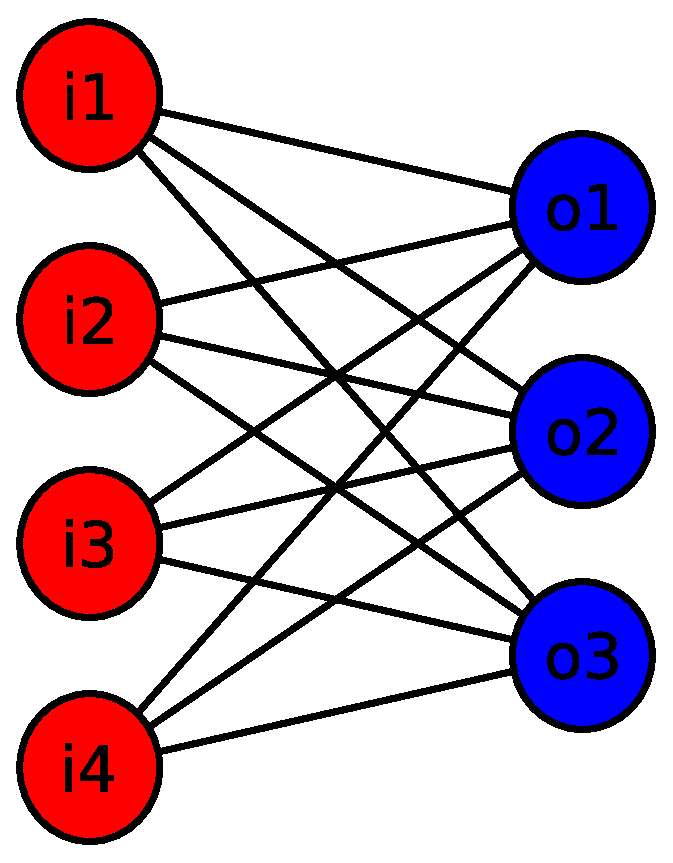
\includegraphics[width=0.7\textwidth]{ann1}
        \caption{A simple neural network with single layer that is the output layer of size three output nodes formed from four input layers and no hidden layer}\label{fig:ann1}
    \end{subfigure}
    \begin{subfigure}[b]{0.48\textwidth}
        \centering
        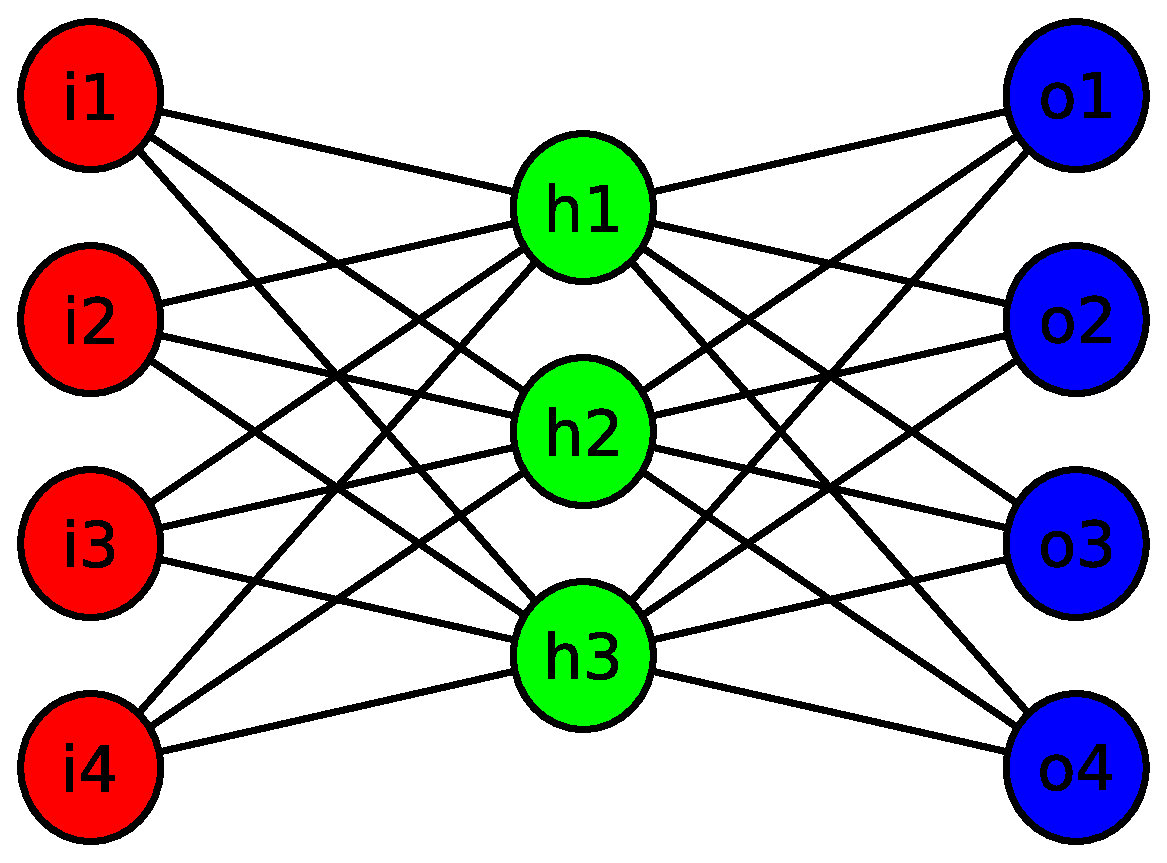
\includegraphics[width=\textwidth]{ann2}
        \caption{A neural network with a single hidden layer of size three between four input nodes and four nodes outputs}\label{fig:ann2}
    \end{subfigure}
\caption{Two simple neural networks, input in red, output in blue.}\label{fig:ann}
\end{figure}


The weighted summation can be expressed in the form of matrix multiplication.
That is given input \(I\) of size \(n\) written as \(I_{n\times 1}\),
output of size \(m\) written as \(O_{m\times 1}\),
the weights \(W_{m\times n}\), and bias values \( B_{m\times 1} \), and activation function \( F \)
The output of the perceptron is defined by formula \ref{eq:perceptron}

\begin{equation}
O_{m\times 1} = F( W_{m\times n} \times I_{n\times 1} + B_{m\times 1} )
\label{eq:perceptron}
\end{equation}

The most basic form of activation function \(F(x)\) is a simple threshold as in \ref{eq:relu} denoted as \( [x]^+ \),
if the weighted summation plus the bias is greater than zero, it's kept as is (activated),
otherwise it's zero (deactivated). The value of the bias controls the threshold.
This form of activation function is called
\gls{relu}\autocite{hahnloser2001permitted}\autocite{jarrett2009best}\autocite{nair2010rectified}

\begin{equation}
f( x ) = [ x ]^+ = max(0, x)
\label{eq:relu}
\end{equation}

There exist many other forms of activation functions like ``Sigmoid functions''\autocite{orr1998neural}\autocite{lecuniefficient}

\begin{equation}
f( x ) = \frac{ 1 }{ 1+e^{-x} }
\label{eq:tanh}
\end{equation}

\begin{equation}
f( x ) = \tanh(x)
\label{eq:tanh}
\end{equation}

\begin{equation}
f( x ) = \tanh(x) + a\cdot x
\label{eq:tanh_plus_linear}
\end{equation}

A common setting for ``Scaled hyperbolic tangent''\autocite{lecun1989generalization} in \ref{eq:scaled_tanh}
is to have \(A=1.7159\) and \(S=2/3\), which would result \(f(1)=1\) and \(f(-1)=-1\).

\begin{eqfloat}
\begin{equation}
f( x ) = A \cdot \tanh(S\cdot x)
\label{eq:scaled_tanh}
\end{equation}
\caption{Scaled hyperbolic tangent. Source:\autocite{lecun1989generalization}}
\end{eqfloat}

A multi-layer neural network is merely a concatenation of simple ones,
the neural network first generate an intermediate state
called hidden layer, then that hidden layer is then become an input of another stage as seen in figure \ref{fig:ann2}.
One can add many intermediate hidden layers.
``Deep Neural Network'' is that with more than one hidden layer.
 
The training process is composed of two phases, forward pass (or forward propagation), and ``Back propagation''.
Parameters (weights and bias values) are randomly initialized, then in forward pass,
each input instance is passed through the \gls{ann}, and compared against the desired output
using some cost function like mean squared error \(E\)
and used to adjust weights accordingly as in figure \ref{fig:bp},
that's why training process is a form of optimization problems with objective to minimize the cost function.

\begin{figure}[!h]
\centering
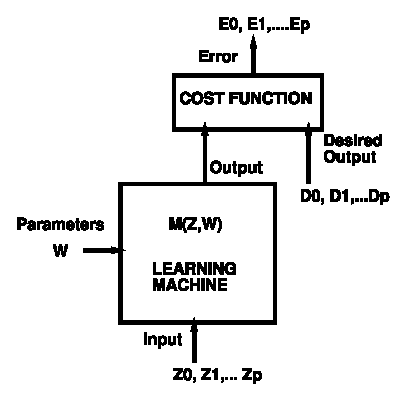
\includegraphics[width=2in]{bp}
\caption{Gradient based learning.}\label{fig:bp}
{Source: \autocite{lecuniefficient}\autocite{orr1998neural}\hfill}
\end{figure}

When having \(n\) layers, the input is denoted as \(X_0\),
the output of first hidden layer is \(X_1\), the last output of the whole network is \(X_n\).
Output can be expressed as a recursive formula \ref{eq:ann_ouput} as in\autocite{lecuniefficient}\autocite{orr1998neural}

\begin{equation}
X_n = F_n(W_n, X_{n-1})
\label{eq:ann_ouput}
\end{equation}

Typically \(F_n\) is the activation function applied to the matrix multiplication of weights to input.

\begin{equation}
X_n = sigmoid( W_n \times X_{n-1}) )
\label{eq:ann_as_matrix}
\end{equation}

\begin{equation}
y = X_n
\end{equation}

\begin{equation}
E = \frac{1}{2} \sqrt{ ( y_{d} - y )^2 }
\end{equation}

A fraction of difference between the desired result and the obtained result is carried backward
(thus the name ``Back propagation'') to adjust the weights,
that fraction is called ``Learning Rate'' in \ref{eq:weights_update} it's \(\eta\)
which can be a constant like 0.01 or some faded value through out the process.
This process is called ``gradient descent''.

\begin{equation}
W(t) = W(t-1) - \eta \cdot \frac{\partial E}{\partial W}
\label{eq:weights_update}
\end{equation}

\begin{equation}
\Delta W = - \eta \cdot \frac{\partial E}{\partial W}
\end{equation}

Taking a random instance (or a very small random subset of training data)
at each step then this is called \gls{sgd}.
Streaming instances and doing the update as they come is called ``online learning''.

\section{Neural Networks for Classification}\label{sec_nn_classification}

Taking the classical example of Iris database, which have four input features
and a corresponding label that has three possible values.
Each one of the three possible classes is made into an output node in the neural network,
and ``Hot One Encoding'' is used to represent it, like this:

\begin{enumerate}
\item ``Setosa'' is represented as \( \begin{bmatrix}1 & 0 & 0\end{bmatrix}^T \)
\item ``Versicolour'' is represented as \( \begin{bmatrix}0 & 1 & 0\end{bmatrix}^T \)
\item ``Virginica'' is represented as \( \begin{bmatrix}0 & 0 & 1\end{bmatrix}^T \)
\end{enumerate}

Only one output node is activated that correspond to the desired class/label.

Normalized exponential function (Softmax)\ref{eq:softmax} is used to convert the open-ended actual output
into probability-like output, because softmax has to important properties\autocite{nasrabadi2007pattern}

\begin{itemize}
\item each output in the interval [0, 1]
\item the summation of all output values is 1.
\end{itemize}

\begin{equation}
softmax(o_j) = \frac{e^{o_j}}{ \sum\limits_{i=1}^n e^{o_i} }
\label{eq:softmax}
\end{equation}

One problem of this, is that it would boost otherwise negligible values as it has to make the summation equal to 1,
for example, given two output nodes having 0.01 and 0.001 the softmax will map them into 50.2\% and 49.8\%.
When given a picture of a tree in a cat or dog task, the probability of being a cat or being a dog
would always be high, it's either a cat or a dog, it would never return a number smaller than some threshold
indicating none of them.

\section{Generalization}

If one made a ML learning model that memorize all the training dataset,
then it would be wrongly considered accurate as it would fail to generalize
and when presented with input that was not part of training data it would fail miserably
this is called ``Over-fitting''.
To measure this, part of the dataset is put aside into ``test dataset''
that is never presented during training but rather used later to evaluate the model.

In case of mini batches with \gls{sgd}, each small batch is also shuffled and split into training and validating dataset.

Regularization\autocite{ng2004feature} tend to prefer smaller weights like the green curve in figure \ref{fig:regularization},
by adding a scalar multiple of weights magnitude summation to the loss function, either absolute value as in ``L1 Regularization''\ref{eq:l1}
or squared as in ``L2 Regularization''\ref{eq:l2} or both\ref{eq:l12}. The scaler \(\lambda\) is called ``Regularization Penalty''.


\begin{equation}
C_{l1} = C + \lambda \sum\limits_{i} | w_i |
\label{eq:l1}
\end{equation}

\begin{equation}
C_{l2} = C + \lambda \sum\limits_{i} w_i^2
\label{eq:l2}
\end{equation}

\begin{equation}
C_{l12} = C + \lambda_1 \sum\limits_{i} | w_i | + \lambda_2 \sum\limits_{i} w_i^2
\label{eq:l12}
\end{equation}


\begin{figure}[!h]
\centering
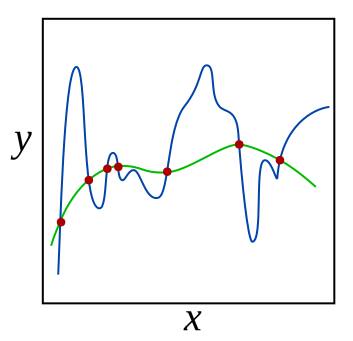
\includegraphics[width=2in]{regularization}
\caption{Two curves that have same loss of zero. Green one have smaller weights, blue one have higher weights. }\label{fig:regularization}
{Source: \href{https://commons.wikimedia.org/wiki/File:Regularization.svg}{Wikipedia}\hfill}
\end{figure}

Another method to force the neural network to generalize is to introduce noise in the training dataset.
Another method is to randomly drop parts of the signal, which is called ``dropout layer''

\section{Convolutional Neural Networks}

\gls{cnn} or more commonly ConvNets was inspired by how
visual cortex is assumed to work. \gls{cnn} is similar to \gls{ann} but uses Convolutional Matrix operator.
The 3D volume formed by multiple 2D matrices channels is called a ``Tensor'',
Given an input image in the form of a Tensor formed by of multiple 2D matrices of pixels for each color channels,
several filters can be written in the form of convolution matrix like edge detection (as in figure \ref{fig:conv-edge}),
sharpen, smoothing/blurring (as in figure \ref{fig:conv-blur}), and pattern matching.
\gls{ann} can be used to learn the values in many convolutional matrices resulting in image filters that
activate when being exposed on specific visual features or structures.

End-to-End solutions feed unprocessed input directly without much prepossessing (if any at all)
and get the end desired result and \gls{nn} is good at that.

The size of each convolutional filter matrix which is also called the ``kernel size'' or the ``neighborhood size''
specifies the receptive field of the filter.
For example, a kernel of size 3×3 means that bounding box of neighborhood starts one pixel to left, one pixel to top
and ends on one pixel to the right and one pixel to the bottom while 5×5 kernel size means two pixels neighborhood
from each side. 

\begin{figure}[!htbp]
\centering
    \begin{subfigure}[b]{0.32\textwidth}
        \centering
\[
\begin{bmatrix}
0 & -1 & 0 \\
-1 & +4 & -1 \\
0 & -1 & 0 
\end{bmatrix}
\]
    \end{subfigure}
    \begin{subfigure}[b]{0.32\textwidth}
        \centering
        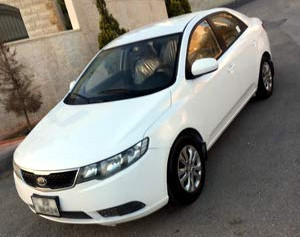
\includegraphics[width=\textwidth]{car}
    \end{subfigure}
    \begin{subfigure}[b]{0.32\textwidth}
        \centering
        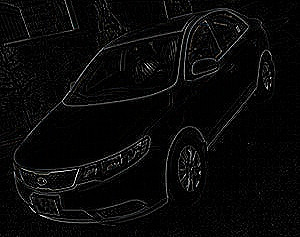
\includegraphics[width=\textwidth]{car-conv-edge}
    \end{subfigure}
\caption{Laplacian operator (edge detection) written as 3×3 convolutional matrix}\label{fig:conv-edge}
\end{figure}

\begin{figure}[!ht]
\centering
    \begin{subfigure}[b]{0.32\textwidth}
        \centering
\[ \begin{aligned}
\frac{1}{16}\cdot
\begin{bmatrix}
1 & 2 & 1 \\
2 & 4 & 2 \\
1 & 2 & 1 \\
\end{bmatrix}
\end{aligned} \]
    \end{subfigure}
    \begin{subfigure}[b]{0.64\textwidth}
        \centering
        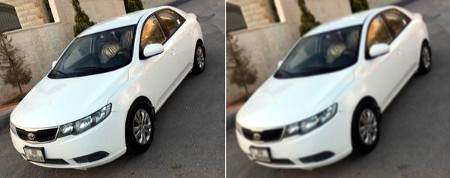
\includegraphics[width=\textwidth]{car-blurred}
    \end{subfigure}
\caption{A blur filter written as 3×3 convolutional matrix}\label{fig:conv-blur}
\end{figure}

The convolution operator used in \gls{cnn} is called 2D convolution
(usually named ``conv2d()'' or ``conv\_2d()'' depending on the used software package)
and it operates on 3D volumes (taking a 3D volume as input and resulting a 3D volume as output)
For example, an input can be a colored image of size 224×224 and depth of 3 RGB channels
(written as \(224×224×3\) or \(3@224×224\)\autocite{lecun1998gradient}),
when passed to a convolution on a neighborhood size 3×3 and depth of 96 channels (written as \(3×3×96\) or \(96@3×3\))
result would be an output volume of size 224×224 (or 222×222 in case of no padding) and depth of 96.
The size of the input is \(width\times height \times depth\) or for short \(W_i\times H_i\times D_i\).
And the output size is \(W_o\times H_o\times D_o\).
The depth of the convolution kernel represent how many filters do we want to apply/learn.

Gray-scale images have input depth of one, but even in that case we still need to operate in 3D volumes,
because we don't want to learn a single filter, after first convolution we would have an output of 3 axis.

Convolution depth varies from layer to layer but input depth of
a layer must match output depth of the previous layer as they work in a pipeline.

So passing an image of size \( W_i\times H_i \) and input depth \( D_i \) (ex. \( D_i=3 \) for RGB channels)
to a convolution layer of kernel size \(W_k\times H_k\) and output depth \(D_o\) would have number of weights
to be learned is \( W_k\times H_k \times D_o \times D_i \) plus \(D_o\) bias values.

You can think of convolution layers as an operator that takes a 3D volume of \(W_i\times H_i\times D_i\)
and result a 3D volume of \(W_i\times H_i\times D_i\) and this operator is to be applied to every possible pixel
in the image by starting from top-left corner (in case of padding), where the neighborhood window is centered,
and slide that window one pixel until all input image is covered. 

In summary a convolution layer has the following properties:

\begin{description}
\item [Input volume size:] \(W_i\times H_i\times D_i \)
\item [Kernel size:] \( W_k\times H_k\times D_o \)
\item [Output volume size:] \( W_o\times H_o\times D_o = W_i\times H_i\times D_o \)
\item [Number of parameters:] are
\begin{itemize}
\item \( W_k\times H_k\times D_o\times D_i \) weight values
\item \( D_o \) bias values
\end{itemize}
\item [Number of window positions:] \( P = W_o\times H_o \)
\item [Number of multiplications in a given position:] \( W_k\times H_k\times D_o\times D_i \)
\item [Number of addition operations in a given position:] \( W_k\times H_k\times D_i\times D_i\) (and another one for bias)
\item [Total number of multiplication operations] \( W_o\times H_o\times W_k\times H_k\times D_o\times D_i\) and same value for addition operations
\end{description}

In case of no padding, convolution start at offset \( =\frac{W_k-1}{2} \) pixels (and a similar offset to the end)
which would be make output smaller by \(W_k-1\) that is \(W_{i}-W_{k}+1\) so with height.

The final objective of all convective convolution operators after all layers of any CNN is
to get us to the desired labels of the classification task, that is \(D_o\)
of the last layer is either the labels or flat features that are being fed to usual \gls{ann} (called Fully Connected layers).

An important special case of no-padding convolution is the case when kernel size matches input size,
that is \(W_i=W_k\) then the output width would be \(W_{i}-W_{k}+1=W_i-W_i+1=1\),
similarly with the height, then the size of the output would be 1×1.
Which converts the 3D volume into one dimension along the depth,
making it suitable to be considered to correspond to the desired labels in the classification task or
to flat features to be fed to usual \gls{ann}.

Another important note that 1×1 convolution with depth \(D_o\)
have the same effect of a hidden layer of size \(D_o\) in usual \gls{ann}.

\begin{itemize}
\item Input volume size: \(1 \times 1 \times D_i \)
\item Output volume size: \( 1 \times 1 \times D_o \)
\item Number of parameters:
    \begin{itemize}
    \item \( D_i \times D_o \) weight values
    \item \( D_o \) bias values
    \end{itemize}
\item Number of window positions: \( P = 1 \times 1 = 1 \)
\item Total number of multiplication operations = \( D_i\times D_o \) and same value for addition operations
\end{itemize}

Some designs may involve sliding more than one pixel at a time, which is a hyper-parameter called ``Stride''
and usually written as \(/S\), for example a kernel of \(5×5×96/3\) means it has width and height of five,
depth of 96 and stride of 3.
And it's a technique used to reduce number of operators (but it does not reduce number of weights).
With a stride value of two output width and height halves. With a Stride of one it's like having no stride.

\begin{description}
\item [Input volume size:] \( W_i\times H_i\times D_i \)
\item [Kernel size:] \( W_k\times H_k\times D_o / S \)
\item [Output volume size:] \( \frac{W_i}{S} \times \frac{H_i}{S} \times D_o \)
\item [Number of parameters:] are
\begin{itemize}
\item \(W_k\times H_k\times D_o\times D_i \) weight values
\item \(D_o\) bias values
\end{itemize}
\item [Number of window positions:] \( P = W_i\times H_i / S^2 = W_o\times H_o \)
\item [Number of multiplications in a given position:] \( W_k\times H_k\times D_o \times D_i \)
\item [Number of addition operations in a given position:] \( W_k\times H_k\times D_i\times D_o\) (including one for bias)
\item [Total number of multiplication operations:] \(W_o\times H_o\times W_k\times H_k\times D_o\times D_i \) and same value for addition operations
\end{description}

The effect of stride is not limited to reducing number of multi-add operations but on the exponential
effect of reducing the output volume of this filter becoming input filter of next layers, for example
applying five layers of convolution with stride of two would reduce width and height of 224×224 into 7×7, because \(224/(2^5)=7\).

\section{No weights layers}

In CNN, not all layer have weights.
Pooling layers have a neighborhood window size and a stride \(S\) written as \(W_k\times H_k / S\).
It uses some aggregate operator like maximum or average to summarize the signal in that window,
that is moved \(S\) pixels each time, resulting on a down-sampled image.
For example average pooling of size 2×2 and stride of 2 (written as 2×2/2)
would have the effect of down-sampling the input image by factor 2.
Pooling is possible with window size not matching the stride,
and is also possible without stride at all (\(S=1\))
that is to summarize surrounding input signals in the window.

The difference of applying stride in convolution or in a pooling layer after it,
is that the first one ignores some input signals while the other one takes the strongest signal (in case of max-pooling).

Another form of no-weights layers is to apply some activation function on input like ``Rectifier Layer''
which applies \gls{relu}\autocite{hahnloser2001permitted}\autocite{jarrett2009best}\autocite{nair2010rectified} to input as in formula \ref{eq:relu}.
Such layers does not affect the shape of its input volume.

\section{Design of CNN models}

A typical basic design of a \gls{cnn} model starts with an input image of certain width and height \(W_{i}\times H_{i}\)
in case of colored images that is a volume of size \(W_{i}\times H_{i}\times 3\).
Then that volume is feed to a sequence of convolution layers of certain kernel size and depth (number of filters).
Then comes a pooling layer (maximum pooling or average pooling), then that is repeated alternating convolution and pooling layers.

The objective of the design is to form a flat signal of no spacial dimension (width=1 and height=1)
but rather along the depth which will be the signal of output classes.
To reduce the width and the height of the signal volume, stride is used on convolution layer or pooling layers.
Different designs of CNN models use stride at different stages, it can be placed early,
down-sampling the signal too early will trade accuracy with speed.

Toward end of the model, either pooling or convolution of kernel size
matching the size of the input will summarize the signal into the desired flat signal of size \(1\times 1\).
When the signal is flat along the depth (having width and height equal to one),
classical \gls{ann} can be used, this is called fully connected layers,
this is equivalent of convolution of kernel size \(1\times 1\).

The last signal is processed with Softmax function as in equation \ref{eq:softmax} to make output signal
form probabilistic-like values as previously discussed in section \ref{sec_nn_classification}.

Figure \ref{fig:cnn-flowchart} shows the whole process of such design.

\begin{figure}[!ht]
\centering
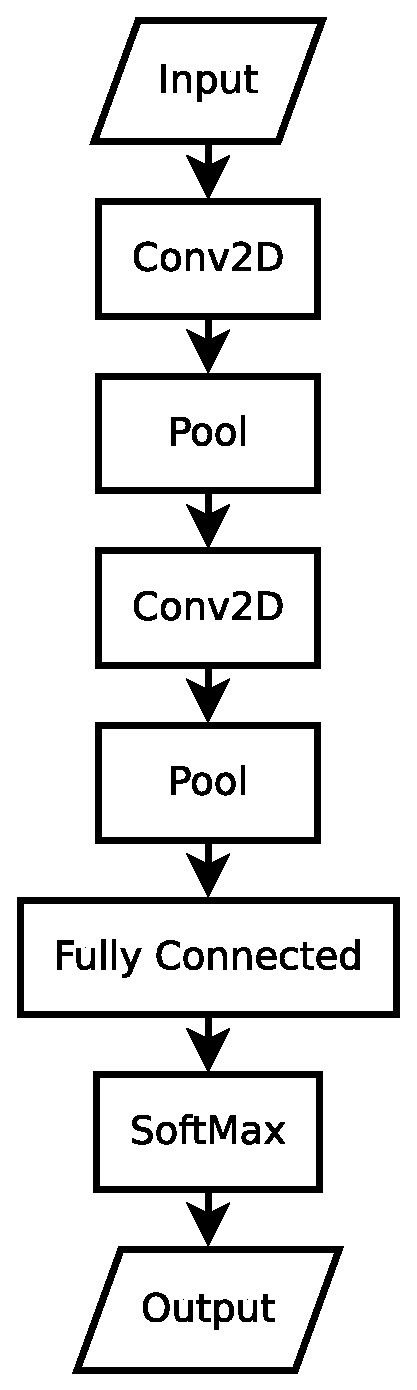
\includegraphics[width=2in]{cnn-flowchart}
\caption{A simple CNN design.}\label{fig:cnn-flowchart}
\end{figure}


\section{Batch Normalization Layers}

Just like it's important to normalize input signal (for example, by subtracting mean and dividing by variance),
it's also important to regulate hidden layers signals.
A batch normalization layer\autocite{ioffe2015batch} is placed after some hidden layers,
having two trainable parameters that are called ``scale'' and ``shift'',
which is updated for each mini-batch in training phase, by finding batch mean and variance.

Some researches suggest using larger mini-batches\autocite{goyal2017accurate}.

\section{Separable Operators}

One of the methods used to reduce number of weights is to decompose the kernel from
being of size \( n \times m \) into two matrices of size \( n \times d \) and \( d \times m \)
and typically \( d=1 \), in this case the number of weights would be
\( (n\times 1)+(1\times m)=n+m\) instead of \(n\times m\)
(or \(2 \cdot n\) instead of \(n^2\) when width and height are equal).
For example one can write a \(3\times 3\) blur kernel using
two matrix multiplication of size \(3\times 1\) and \(1\times 3\) as in (\ref{eq:sep_blur}),
there are a total of six weights in two matrices (3×1 and 1×3) compared to nine in the equivalent 3×3 matrix.

\begin{eqfloat}
\begin{equation}
\begin{bmatrix}
1 \\
2 \\
1
\end{bmatrix}
\times
\begin{bmatrix}
1 & 2 & 1
\end{bmatrix}
=\begin{bmatrix}
1 & 2 & 1 \\
2 & 4 & 2 \\
1 & 2 & 1 \\
\end{bmatrix}
\label{eq:sep_blur}
\end{equation}
\caption{ 3×3 blur operator written as two matrices each of three }
\end{eqfloat}

Beside being used along the width and height of the convolution kernel it can be used along kernel depth
where the convolution kernel of \( W_k \times H_k \) that takes input of depth \(D_i\)
and output depth of \(D_o\) using intermediate value called depth multiplayer \(D_M\) and which can be 1.
One way of doing this is two consecutive convolutions one is called\autocite{chollet2016xception}\autocite{mamalet2012simplifying}
``depth-wise convolution'' that operate on a kernel of 3×3 on an intermediate depth of \(D_M\) (typically 1)
and the other is called ``point-wise convolution'' that operate on a kernel of 1×1 with output depth of \(D_o\)

\newcommand{\ra}[1]{\renewcommand{\arraystretch}{#1}}

\begin{table*}\caption{How separable operators reduce number of weights and multiplications}\label{table:sep_op}
\centering
\begin{small}
\begin{tabularx}{\textwidth}{cccccrX}
\toprule
Name & Input & depth & kernel & depth & weights & mults \\
\midrule
original & 224×224 & 3 & 3×3 & 96 & 3×3×3×96 =2,592 & 224×224×3×3×3×96 = 130.1M \\
\bottomrule
\multicolumn{7}{c}{Separable equivalent} \\
\midrule
depth-wise & 224×224 & 3 & 3×3 & 1 & 3×3×3×1 =27 & 224×224×3×3×3×1 =1.4M \\
\midrule
point-wise & 224×224 & 1 & 1×1 & 96 & 1×1×1×96 =96 & 224×224×1×1×1×96 =4.8M \\
\cmidrule{5-7}
\multicolumn{5}{r}{Total} & 27+96 =123 & 6.2M \\
\bottomrule
\end{tabularx}
\end{small}
\end{table*}

\begin{table*}\caption{Separable operators reduction applied to hidden layer}\label{table:sep_hidden}
\centering
\begin{small}
\begin{tabularx}{\textwidth}{cccccrX}
\toprule
Name & Input & depth & kernel & depth & weights & mults \\
\midrule
original & 224×224 & 64 & 3×3 & 64 & 64×3×3×64 =36,864 & 224×224×64×3×3×64 =1,849.7M \\
\bottomrule
\multicolumn{7}{c}{Separable equivalent of same hidden layer} \\
\midrule
depth-wise & 224×224 & 64 & 3×3 & 1 & 64×3×3×1 =576 & 224×224×64×3×3×1 =28.9M \\
\midrule
point-wise & 224×224 & 1 & 1×1 & 64 & 1×1×1×64 =64 & 224×224×1×1×1×64 =3.2M \\
\cmidrule{5-7}
\multicolumn{5}{r}{Total} & 640 & 32.1M \\
\bottomrule
\end{tabularx}
\end{small}
\end{table*}

As we can see table \ref{table:sep_op} when have an input image of size 224×224 and 3 RGB channels
which is convolved with 3×3 kernel and 96 filters (output depth),
then typically we have 2.5K weights and 130M multiplications.
A separable counterpart of 3×3×1 and 1×1×96 with same input volume
and output volume would have only 123 weights and 6M weights.
In the second case as in table \ref{table:sep_hidden} when we take an input volume of size 224×224×64 to be convolved with a kernel of 3×3
and an output depth of 64, the usual convolution have 36K weights and 1,800M multiplications.
On the other hand the separable version of \(D_M=1\) have only 640 weights and 32M multiplications.

\section{Accuracy Metrics}

\begin{description}
\item [Accuracy rate] which is the ratio of true items, both true positives (\(T_P\))
and true negatives (\(T_N\)) over total (or its complement ``Error rate'' which is the ratio of false items both
false positives \(F_P\) and false negatives \(F_N\) over total).
Those two metrics are vulnerable if the likelihood of labels are not equal.
For example, if the problem domain is diagnosing cancer,
assuming that the probability of cancer is small like 0.1\%,
a classifier that randomly pick cancer positives with very small probability or even not report any cancer positive at all
(classify every body as healthy) would have very high accuracy (99.9\%)
and low error rate (since it only mistaken people with cancer, so it have error rate of 0.1\%).
To overcome this, a metric (like ``Precision'' and ``Recall'' below) is needed
that does not consider success rate or failure compared
to total, but makes the denominator to be limited to smaller context.  
\begin{equation}
Accuracy = \frac{ T_P + T_N}{ SampleSize }
\label{eq:precision}
\end{equation}
\item [Precision] is the ratio of true positive items over positively diagnosed items (both \(T_P\) and \(F_P\)),
which is a measure of Type I error caused by the \(F_P\) in the denominator \ref{eq:precision}.
\begin{equation}
Precision = \frac{ T_P }{ T_P + F_P }
\label{eq:precision}
\end{equation}
\item [Recall] is the ratio of true positive items compared all positive items
(both truly diagnosed and falsely missed), which is a measure of Type II error that cases the \(F_N\) in the denominator \ref{eq:recall}.
\begin{equation}
Recall = \frac{ T_P }{ T_P + F_N }
\label{eq:recall}
\end{equation}
\end{description}

In the above example of random cancer diagnose that picks 0.1\%, in a sample of 10,000 person,
it would randomly diagnose ten persons with cancer, but only one of them actually have cancer
and it missed eight persons that diagnosed as healthy despite that they actually have cancer
(the rest where accurately diagnosed healthy).

\[accuracy = \frac{ 1 + 9982 }{10,000} = 99.83\% \]
\[precision = \frac{ 1 }{10} = 10.00\% \]
\[recall = \frac{ 1 }{1+8} = 11.11\% \]

\section{Public Datasets and Benchmarks}
\gls{cifar} have published CIFAR-10\autocite{krizhevsky2009learning}
dataset of small \( 32\times 32 \) labeled images of ten classes.

ImageNet\autocite{deng2009imagenet} \gls{ilsvrc}\autocite{deng2012imagenet}\autocite{krizhevsky2012imagenet}
is the benchmark used by state-of-the-art methods.
ILSVRC has many tasks, most notably the classification task of 2012
(\href{http://www.image-net.org/challenges/LSVRC/2012/}{ILSVRC-2012-CLS})
which has one thousand class of objects and large colored images
(compared to CIFAR-10's 32×32, ILSVRC’s 224×224 is 49 times more pixels).

There are other much simpler datasets like the \gls{minst}\autocite{lecun2010mnist}\autocite{lecun1998gradient}
which is a database of 70,000 handwritten digits of size 28×28 pixels that is centered and normalized,
it’s considered easy to achieve 99\% accuracy on this dataset. 

%TBD: databases for fine tuning: flowers, dogs, food 101 datasets

\chapter{Literature Review}

% TODO: consider which parts to move to chapter 3 ex. our calculations or conclusions

\section{CNN Model Design}

Different papers define and draw their CNN design differently,
this research analyses them then represent them into a unified table.

% TBD NOTE: in figures Convention input is put at the bottom and classes at the top or left to right.

\subsection{LeNet}

LeNet\autocite{lecun1998gradient} was one of the first successful ConvNets. 
It was used to recognize characters (thus domain specific),
the research was based on NIST Special Database 1 (SD-3)\autocite{wilson1990nist}
and NIST Special Database 3 (SD-3)\autocite{garris1992nist}
and their research resulted in one of the most infamous databases;
the Modified National Institute of Standards and Technology(MNIST) database\autocite{lecun2010mnist}.

Their CNN operates on a gray-scale input of 32×32 pixels (or 28×28 surrounded with 4 padding pixels),
input images were pre-processed to be centered, normalized, segmented ..etc.
First convolution is applied without padding, it has kernel size 5×5 (two pixels from each side around center)
which would output a volume of size 28×28. In the initial paper they used output
depth of 6 for the first convolution layer as shown in figure \ref{fig:lenet} from same paper.

In other words, first layer would train six kernels each of size 5×5 transforming
a volume of 32×32×1 input (depth is 1 not 3 because it's input is not colored)
into an output of 28×28×6.

LeNet-5 has seven layers as seen in figure \ref{fig:lenet},
five of them have trainable weights and two layers of them do not have weights.

Table \ref{table:lenet-cnn} demonstrates operations done on each layer and the corresponding number of parameters
to be trained (weight and bias values) and number of multiplications operations
(same number of addition operations) in each layer

\begin{figure}[!h]
\centering
\includegraphics[width=5in]{lenet}
\caption{LeNet-5 CNN desgin}\label{fig:lenet}
{Source: \autocite{lecun1998gradient}\hfill}
\end{figure}


\begin{table*}\caption{Details of LeNet layers, their input size, kernel size, output size and number of parameters (weights and bias).  W×H×D/S stands for width, height, depth and stride respectively}\label{table:lenet-cnn}
\centering
\begin{small}
\begin{tabularx}{\textwidth}{llllXX}
\toprule
Layer & Input & Kernel & Output & Params & Mults \\
Name & W×H×D & W×H×D/S & W×H×D & &  \\
\midrule
C1: conv2d & 32×32×1 & 5×5×6 &  28×28×6 & 1×5×5×6+6 =156 & 28×28×1×5×5×6 =117,600 \\
S2: pool/2 & 28×28×6 & 2×2/2 &  14×14×6 & 0 & 0 \\
C3: conv2d & 14×14×6 & 5×5×16 & 10×10×16 & 6×5×5×16+16 =2,416 & 10×10×6×5×5×16 =240,000 \\
S4: pool/2 & 10×10×16 & 2×2/2 &  5×5×16 & 0 & 0 \\
C5: conv2d & 5×5×16 & 5×5×120 &  1×1×120 & 16×5×5×120+120 =48,120 & 1×1×16×5×5×120 =48,000 \\
F6: conv2d & 1×1×120 & 1×1×84 &  1×1×84 & 120×1×1×84+84 =10,164 & 120×84 =10,080 \\
F7: conv2d & 1×1×84 & 1×1×10 &   1×1×10 & 84×1×1×10+10 =850 & 84×40 =840 \\
\cmidrule{4-6}
\multicolumn{4}{r}{Total} & 61,706 & 416,520 \\
\bottomrule
\end{tabularx}
\end{small}
\end{table*}

Despite having a simple design, shallow depth and specific simple task operating on a pre-processed normalized input,
it has more than 61k parameters and about half million multiplication operation and half million addition operations.
F6 is a fully connected hidden layer and F7 is the fully connected output layer,
the output depth of last layer is the number of classes in this example that is the ten digits from 0-9.
Another note that will be commonly seen in this research that most weights are in layer that flatten its input into 1×1 just before fully connected layers,
in LeNet it's C5 with 78\% of weights.

Note: Because bias values is very small compared to weights as we have seen above, we would only show weights. 

\subsection{AlexNet}

AlexNet\autocite{krizhevsky2012imagenet} was the winner of ILSVRC in 2012,
the design of this ConvNet is demonstrated in figure \ref{fig:alexnet} which shows half of it which is running
on one GPU having a similar copy runs on another GPU, for example, on the left it starts with an input image
and pass it through 11×11 kernel of depth 48 on one GPU and another same sized depth on the other GPU, 
resulting total of 96 filters to be learned. 

AlexNet main contribution is the use two GPUs in parallel with less communication between them
and the reduction of over-fitting with data augmentation and dropout.

\begin{figure}[!h]
\centering
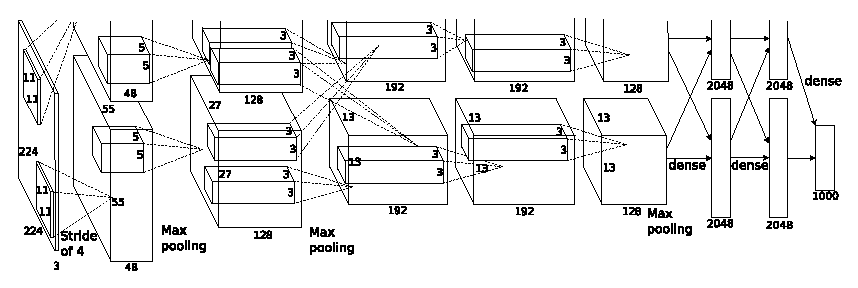
\includegraphics[width=5in]{alexnet}
\caption{AlexNet running on two GPU cores}\label{fig:alexnet}
{Source: \autocite{lecun1998gradient}\hfill}
\end{figure}

A slightly modified version of AlexNet (called AlexNet v2\autocite{krizhevsky2014one}) is shown
in the table \ref{table:alexnet-cnn}

\clearpage
\begin{landscape}
\clearpage
\centering

\begin{table*}\caption{Analysis of AlexNet v2 layers, showing input size, kernel size, output size and number of weights and multiplications and their percent. Kernel size is width, height, depth and stride in the form of WxHxD/S}\label{table:alexnet-cnn}
\centering
\begin{tabularx}{\hsize}{Xlllrrrr}
\toprule
Layer & Input & Kernel & Output & Weights & \% & Mults & \% \\
\midrule
c1: conv2d/4 & 224×224×3 & 11×11×64/4 & 54×54×64 & 3×11×11×64 & 0\% & 54×54×3×11×11×64 & 9.2\% \\
pool/2 & 54×54×64 & 3×3/2 & 26×26×64 & 0 & 0 & 0 & 0 \\
c2: conv2d & 26×26×64 & 5×5×192 & 26×26×192 & 64×5×5×192 & 0.6\% & 26×26×64×5×5×192 &  \textbf{28.2\%} \\
pool/2 & 26×26×192 & 3×3/2 & 12×12×192 & 0 & 0 & 0 & 0 \\
c3: conv2d & 12×22×192 & 3×3×384 & 12×12×384 & 192×3×3×384 & 1.3\% & 12×12×192×3×3×384 & 13.0\% \\
c4: conv2d & 12×12×384 & 3×3×384 & 12×12×384 & 384×3×3×384 & 2.6\% & 12×12×384×3×3×384 & 25.9\% \\
c5: conv2d & 12×12×384 & 3×3×256 & 12×12×256 & 384×3×3×384 & 1.8\% & 12×12×384×3×3×384 & 17.3\% \\
pool/2 & 12×12×256 & 3×3/2 & 5×5×256 & 0 & 0 & 0 & 0 \\
fc6 & 5×5×256  & 5×5×4096 & 1×1×4096 & 256×5×5×4096 &  \textbf{52.1\%} & 1×1×256×5×5×4096 & 3.6\% \\
fc7 & 1×1×4096 & 1×1×4096 & 1×1×4096 & 4096×1×1×4096 & 33.4\% & 4096×4096 & 2.3\% \\
fc8 & 1×1×4096 & 1×1×1000 & 1×1×1000 & 4096×1×1×1000 & 8.1\% & 4096×1000 & 0.6\% \\
\cmidrule{5-8}
\multicolumn{4}{r}{total} & 50M & 100\% & 737M & 100\% \\
\bottomrule
\end{tabularx}
\end{table*}

\end{landscape}
\clearpage

\subsection{ZFNet}

ZFNet\autocite{zeiler2014visualizing} (also known as Zeiler \& Fergus architecture)
was the winner of ILSVRC 2013. ZFNet's main contribution is the concept of ``DeConv'',
as they covered part of input image with a gray square to see which part of the image activates which part of the neural network.

This model is slightly modified Alexnet, same depth, same blocks with smaller stride of two at first convolution of four
and smaller filter size of 7 instead of 11, slightly more weights and operations,
for details refer to figure \ref{fig:zfnet} and table \ref{table:zfnet}.

\begin{figure}[!h]
\centering
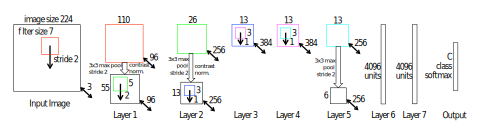
\includegraphics[width=5in]{zfnet}
\caption{ZFNet design}\label{fig:zfnet}
{Source: \autocite{zeiler2014visualizing}\hfill}
\end{figure}

\clearpage
\begin{landscape}
\clearpage
\centering

\begin{table*}\caption{Analysis of ZFNet layers}\label{table:zfnet}
\centering
\begin{tabularx}{\hsize}{Xlllrrrr}
\toprule
Layer & Input & Kernel & Output & Weights & \% & Mults & \% \\
\midrule
c1: conv2d/2 & 224×224×3 & 7×7×96/2 & 110×110×96 & 3×7×7×96 & 0.0\% & 110×110×3×7×7×96 & 14.6\% \\
pool/2 & 110×110×96 & 3×3/2 & 55×55×96 & 0 & 0.0\% & 0 & 0.0\% \\
c2: Conv2d/2 & 55×55×56 & 5×5×256 & 26×26×256 & 96×5×5×256 & 1.0\% & 26×26×96×5×5×256 & \textbf{35.6\%} \\
pool/2 & 26×26×256 & 3×3/2 & 13×13×256 & 0 & 0.0\% & 0 & 0.0\% \\
c3: conv2d & 13×13×256 & 3×3×384 & 13×13×384 & 256×3×3×384 & 1.4\% & 13×13×256×3×3×384 & 12.8\% \\
c4: conv2d & 13×13×384 & 3×3×384 & 13×13×384 & 384×3×3×384 & 2.1\% & 13×13×384×3×3×384 & 19.2\% \\
c5: conv2d & 13×13×384 & 3×3×256 & 13×13×256 & 384×3×3×256 & 1.4\% & 13×13×384×3×3×256 & 12.8\% \\
pool/2 & 13×13×256 & 3×3/2 & 6×6×256 & 0 & 0.0\% & 0 & 0.0\% \\
fc6 & 6×6×256 & 6×6×4096 & 1×1×4096 & 256×6×6×4096 & \textbf{60.5\%} & 256×6×6×4096 & 3.2\% \\
fc7 & 1×1×4096 & 1×1×4096 & 1×1×4096 & 4096×4096 & 26.9\% & 4096×4096 & 1.4\% \\
fc8 & 1×1×4096 & 1×1×1000 & 1×1×1000 & 4096×1000 & 6.6\% & 4096×1000 & 0.4\% \\
\cmidrule{4-8}
\multicolumn{4}{r}{Total} & 62M & 100\% & 1,168M & 100\% \\
\bottomrule
\end{tabularx}
\end{table*}

\end{landscape}
\clearpage

\subsection{VGG}
VGG\autocite{simonyan2014very} came second in ILSVRC 2014, 
The paper discussed many variations named after number of layers with trainable weights
for example VGG16 (variation D in the paper) have has 16 layers with trainable weights,
VGG-16 has 138M weights, 74\% of which are in ``fc6'' layer as seen in table \ref{table:vgg}.

VGG-16 was the best performing variation of VGG, It was better than shallower variations like VGG-11 (variation A)
and deeper variations like VGG-19 (variation E)

\clearpage
\begin{landscape}
\clearpage
\centering
\begin{table*}\caption{Analysis of VGG-16}\label{table:vgg}
\centering
\begin{tabularx}{\hsize}{Xlllrrrr}
\toprule
Layer & Input & Kernel/Stride & Output & Weights & \% & Mults & \% \\
\midrule
Name & Wi×Hi×Di & Wk×Hk×Do/S & Wo×Wo×Do & Wk×Hk×Do×Di & - & Wo×Ho×Wk×Hk×Do×Di & - \\
\midrule
conv1\_1 & 224×224×3 & 3×3×64 & 224×224×64 & 3×3×64×3 & 0.0\% &   224×224×3×3×64×3 & 0.6\% \\
conv1\_2 & 224×224×64 & 3×3×64 & 224×224×64 & 3×3×64×64 & 0.0\% & 224×224×3×3×64×64 & 12.0\% \\
pool/2 & 224×224×64 & 2×2/2 & 112×112×64 & 0 & 0 & 0 & 0 \\
conv2\_1 & 112×112×64  & 3×3×128 & 112×112×128 & 3×3×128×64 & 0.1\% & 112×112x3×3×128×64 & 6.0\% \\
conv2\_2 & 112×112×128 & 3×3×128 & 112×112×128 & 3×3×128×128 & 0.1\% & 112×112x3×3×128×128 & 12.0\% \\
pool/2 & 112×112×128 & 2×2/2 & 56×56×128 & 0 & 0 & 0 & 0 \\
conv3\_1 & 56×56×128 & 3×3×256 & 56×56×256 & 3×3×256×128 & 0.2\% & 56×56×3×3×256×128 & 6.0\% \\
conv3\_2 & 56×56×256 & 3×3×256 & 56×56×256 & 3×3×256×256 & 0.4\% & 56×56×3×3×256×128 & 12.0\% \\
conv3\_3 & 56×56×256 & 3×3×256 & 56×56×256 & 3×3×256×256 & 0.4\% & 56×56×3×3×256×128 & 12.0\% \\
pool/2 & 56×56×256 & 2×2/2 & 28×28×256 & 0 & 0 & 0 & 0 \\
conv4\_1 & 28×28×256 & 3×3×512 & 28×28×512 & 3×3×512×256 & 0.9\% & 28×28×3×3×512×256 & 6.0\% \\
conv4\_2 & 28×28×256 & 3×3×512 & 28×28×512 & 3×3×512×512 & 1.7\% & 28×28×3×3×512×512 & 12.0\% \\
conv4\_3 & 28×28×256 & 3×3×512 & 28×28×512 & 3×3×512×512 & 1.7\% & 28×28×3×3×512×512 & 12.0\% \\
pool/2 & 28×28×512 & 2×2/2 & 14×14×512 & 0 & 0 & 0 & 0\\
conv5\_1 & 14×14×512 & 3×3×512 & 14×14×412 & 3×3×512×512 & 1.7\% & 14×14×3×3×512×512 & 3.0\% \\
conv5\_2 & 14×14×512 & 3×3×512 & 14×14×412 & 3×3×512×512 & 1.7\% & 14×14×3×3×512×512 & 3.0\% \\
conv5\_3 & 14×14×512 & 3×3×512 & 14×14×412 & 3×3×512×512 & 1.7\% & 14×14×3×3×512×512 & 3.0\% \\
pool/2 & 14×14×512 & 2×2/2 & 7×7×512 & 0 &  0 & 0 & 0 \\
fc6: conv2d & 7×7×512 & 7×7×4096 & 1×1×4096 & 7×7×4096×512 & \textbf{74.3\%} & 7×7×4096×512 & 0.7\% \\
fc7: conv2d & 1×1×4096 & 1×1×4096 & 1×1×4096 & 4096×4096 & 12.1\% & 4096×4096 & 0.1\% \\
fc8: conv2d & 1×1×4096 & 1×1×1000 & 1×1×1000 & 4096×1000 & 3.0\% & 4096×1000 & 0.0\% \\
\cmidrule{4-8}
\multicolumn{4}{r}{Total:} & 138M & 100\% & 15,470M & 100\% \\
\bottomrule
\end{tabularx}
\end{table*}
\end{landscape}
\clearpage


\subsection{GoogLeNet or Inception v1}\label{sec_inception_v1}
GoogLeNet (aka \href{https://github.com/google/inception/blob/master/inception.ipynb}{Inception} v1)\autocite{szegedy2015going}, the winner of ILSVRC 2014,
has 22 layer having trainable weights (more than two times deeper than AlexNet v2\autocite{krizhevsky2014one}).
The design of this model is very different as input flows in branches that later get joined using ``DepthConcat''
which as its name suggests places collect the output of different branches along the depth of output volume.
That building block of this design is called ``inception module'' which is shown in figure \ref{fig:inception-block},
their CNN is composed of nine inception blocks
(not to be confused with layers).
Each block has four branches and it's two layers deep (except one branch, which has one layer)

\begin{itemize}
\item 1×1 followed by 3×3
\item 1×1 followed by 5×5
\item Max Pooling of size 3×3 (stride of 1) followed by 1×1
\item 1×1
\end{itemize}


\begin{figure}[!h]
\centering
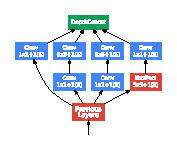
\includegraphics[width=5in]{inception-block}
\caption{An Inception module block}\label{fig:inception-block}
{Source: \autocite{szegedy2015going}\hfill}
\end{figure}


As mentioned before those branches are merged using ``depth concatenation'', for example first inception block takes
input of size 28×28×192 (coming from the output previous convolutions and pooling)
which flows to the four mentioned branches
the 1×1×64 branch outputs 28×28×64, the 3×3×128 branch outputs 28×28×128, the 5×5×32 branch outputs 28×28×32
and the max pool branch outputs 28×28×32 (because pooling stride is 1),
resulting matching output size of 28×28 and total number of depth to be \( 64+128+32+32 = 256 \) in depth.

Separable operators technique has been discussed previously and it's seen here,
instead of making a branch of 3×3×128,
they made it into 1×1×96 followed by 3×3×128 (here depth multiplier is 96).
The table \ref{table:inception-sep3} compares the 3×3 part of first inception block compared to its non-reduced equivalent,
using depth-multiplayer of 96 (reducing input depth from 192 to 96)
and as a result of this reduction number of weights were reduced by about 41.7\% and number of multiplications were reduced by about 41\%. 

Unlike separable operators we have seen before, the 1×1 point-wise stage is placed before the depth-wise stage in Inception.
Table \ref{table:inception-sep5} shows the 5×5 part of first inception block compared to its non-reduced equivalent,
using depth multiplier of 16 (reducing input depth from 192 to 16)
and as a result of this reduction number of weights were reduced by 90\%
and number of multiplications were reduced by 90\%. 


\begin{table*}\caption{Overhead of 3×3×128 convolution in Inception almost halved using separable operators}\label{table:inception-sep3}
\begin{small}
\begin{tabularx}{\textwidth}{ccccXX}
\toprule
\textbf{Name} & \textbf{Input} & \textbf{kernel} & \textbf{output} & \textbf{weights} & \textbf{mults} \\
\midrule
\multicolumn{6}{c}{Separable Version} \\
\midrule
point-wise & 28×28×192 & 1×1×96 & 28×28×96 & 1×1×96×192 & 28×28×96×192 \\
depth-wise & 28×28×96 & 3×3×128 & 28×28×128 & 3×3×128×96 & 28×28×3×3×128×96 \\
\cmidrule{4-6}
\multicolumn{3}{r}{} & \multicolumn{1}{l}{Total} & 129K & 101M \\
\midrule
\multicolumn{6}{c}{Non-separable Version} \\
\midrule
original & 28×28×192 & 3×3×128 & 28×28×128 & 3×3×128×192 =221K & 28×28×3×3×192×128 =173M \\
\bottomrule
\end{tabularx}
\end{small}
\end{table*}


\begin{table*}\caption{Overhead of 5×5×32 convolution in Inception reduce by 90\%}\label{table:inception-sep5}
\begin{small}
\begin{tabularx}{\textwidth}{ccccXX}
\toprule
Name & Input & kernel & output & weights & mults \\
\midrule
\multicolumn{6}{c}{Separable Version} \\
\midrule
point-wise & 28×28×192 & 1×1×16 & 28×28×16 & 1×1×16×192 & 28×28×192×16 \\
depth-wise & 28×28×16 & 5×5×32 & 28×28×32 & 5×5×32×16 & 28×28×5×5×32×16 \\
\cmidrule{5-6}
\multicolumn{4}{r}{} & Total: 16K & 12M \\
\midrule
\multicolumn{6}{c}{Non-separable Version} \\
\midrule
original & 28×28×192 & 5×5×32 & 28×28×32 & 5×5×32×192 =154K & 28×28×5×5×32×192 =120M \\
\bottomrule
\end{tabularx}
\end{small}
\end{table*}

General properties of this design:
\begin{itemize}
\item It can learn a features in a context of 3×3 or 5×5 (receptive fields) at the same layer level
\item It can pass features from different context sizes from layer to layer
(ex. combining a feature of 3×3 from one layer to a feature of 3×3 or 5×5 from previous layer)
increasing and varying the size of receptive field.
\item the use of 1×1 branch is similar in effect to having a fully connected hidden layer
(connecting neurons of input depth to neurons output depth)
but much less expensive because it's used with OD much smaller than ID and since it's an intermediate layer
it can be thought as an intermediate point-wise step in separable operator.
\item No dense fully connected layers just before the classification layer
(other CNN have a hidden layer with 4096 neurons with most of trainable weights)
which is eliminated here and saved more than 70\% of wasted weights (compare that to layer named fc6 in VGG-16 network as seen in table \ref{table:vgg})
\item Has a total of ~6M weights, compared to ~50M in AlexNet (as in table \ref{table:alexnet-cnn}) and ~140M in VGG-16(as in table \ref{table:vgg}) and 1.5G multiplications (compared to 15.4G multiplications in VGG-16) with better accuracy 
\item Their Paper\autocite{szegedy2015going} introduced the notion of ``Auxiliary Classifiers'' as counter measure for vanishing gradient.
Beside the final so deep fully connected layers that is followed by ``softmax'' resulting the probabilities of each class,
they have much earlier side fully connected layers and ``softmax'' towers.
A fraction of the losss of those auxiliary classifiers is added to the final total loss,
in that paper they used 0.3 of the auxiliary loss.
This way, the ConvNet would be able to do the classification task as early as possible before going deeper.
After training is done, those side towers are removed, because they are not needed in classification.
\end{itemize}

\subsection{Inception v2 and v3}

What is common in all inception versions\autocite{szegedy2016rethinking}\autocite{ioffe2015batch}\autocite{chollet2016xception}\autocite{krause2016unreasonable}
is the use of branched later depth-concatenated blocked called ``inception module''
and the use of 1×1 to reduce order. Table \ref{table:inception-ver-1-4} compares all versions of inception.

\begin{figure}[!ht]
\centering
    \begin{subfigure}[b]{0.4\textwidth}
        
\includegraphics[width=\textwidth]{inception-v3-3}
        \caption{An Inception v3 Block}\label{fig:inception-v3-3}
    \end{subfigure}
    \begin{subfigure}[b]{0.4\textwidth}
        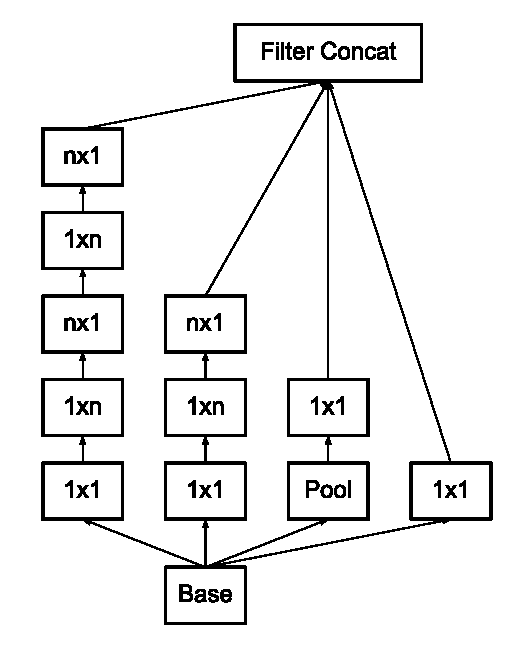
\includegraphics[width=\textwidth]{inception-v3-n}
        \caption{An Inception v3 Block used with \(n=7\)}\label{fig:inception-v3-n}
    \end{subfigure}
\caption{Two variations of Inception v3 blocks }\label{fig:inception-v3}
{Source: \autocite{szegedy2016rethinking}}
\end{figure}



In version two of inception, 5×5 was replaced with 3×3 (as two concatenated 3×3 would have the same receptive field of 5×5)
Also separable convolution is done in this version too early as first layer which produce 64 depth using depth multiplier DM=8.
Beside reduction along the depth, inception v2 introduced reduction along width and height which is called
``Introduced Spatial Factorization'' using
``Asymmetric Convolutions'' that is separating \(k\times k\) kernels into \(k\times 1\) followed by \( 1\times k \).
In Inception v1, all inception blocks were identical while later inception version have many variations of the inception block
one of them having 3×3 followed by 1×1 kernels instead of 3×3 kernel. And another type with 1×1, 7×7, 1×1 then followed by 7×7.
Two variants of this technique is seen in figure \ref{fig:inception-v3}.

Counting layers in inception is tricky and misleading,
because reducing an operator using ``separable operator'' methodology into two or more layers make a less generic filter with more layers.

% TODO: find a better metric to measure depth other than misleading number of layers

\begin{table*}\caption{Comparing all versions of Inception}\label{table:inception-ver-1-4}
\centering
\begin{tabular}{@{}cccccc@{}}
\toprule
Model Name & layers & weights & mults & Top-1 accuracy & Top-5 accuracy \\
\midrule
Inception v1 & 22 & 6.6M & 1,498M & 69.8 & 89.6 \\
Inception v2 & 42 & 11M & 1,934M & 73.9 & 91.8 \\
Inception v3 & 53 & 27M & 5,719M & 78.0 & 93.9 \\
Inception v4 & 81 & 46M & 13,882M & 80.2 & 95.2 \\
Inception ResNet V2 & 130 & 59M & 14,882M & 80.4 & 95.3 \\
\bottomrule
\end{tabular}
\end{table*}

\subsection{Highway Networks}

Deeper networks are more difficult to train due to vanishing gradients, 
a problem which is also faced by Recurrent Neural Networks (RNNs)
that was approached by long short term memory (LSTM) blocks
which uses gates that facilitate information passing from one block to another block as in figure \ref{fig:lstm-chain}.

Inspired by LSTM, Highway Networks\autocite{srivastava2015highway}\autocite{srivastava2015training} 
uses gated information flow in deeper CNNs. Hidden layer output \(H\)
can be suppressed and replaced by passing input \(x\), depending on the value of
a special gate \(T\) which takes a value from zero to one (using sigmoid function)
as in formula \ref{eq:highway}.

\begin{equation}
y = H(x, W_{H} ) \cdot T (x, W_{T} ) + x \cdot (1 - T (x, W_{T} ))
\label{eq:highway}
\end{equation}

By having \(T=0\), the first term will be zero and the second term will be the input \(x\) as is,
that is information bypassing current layer and flow to next deeper layer.


\begin{figure}[!h]
\centering
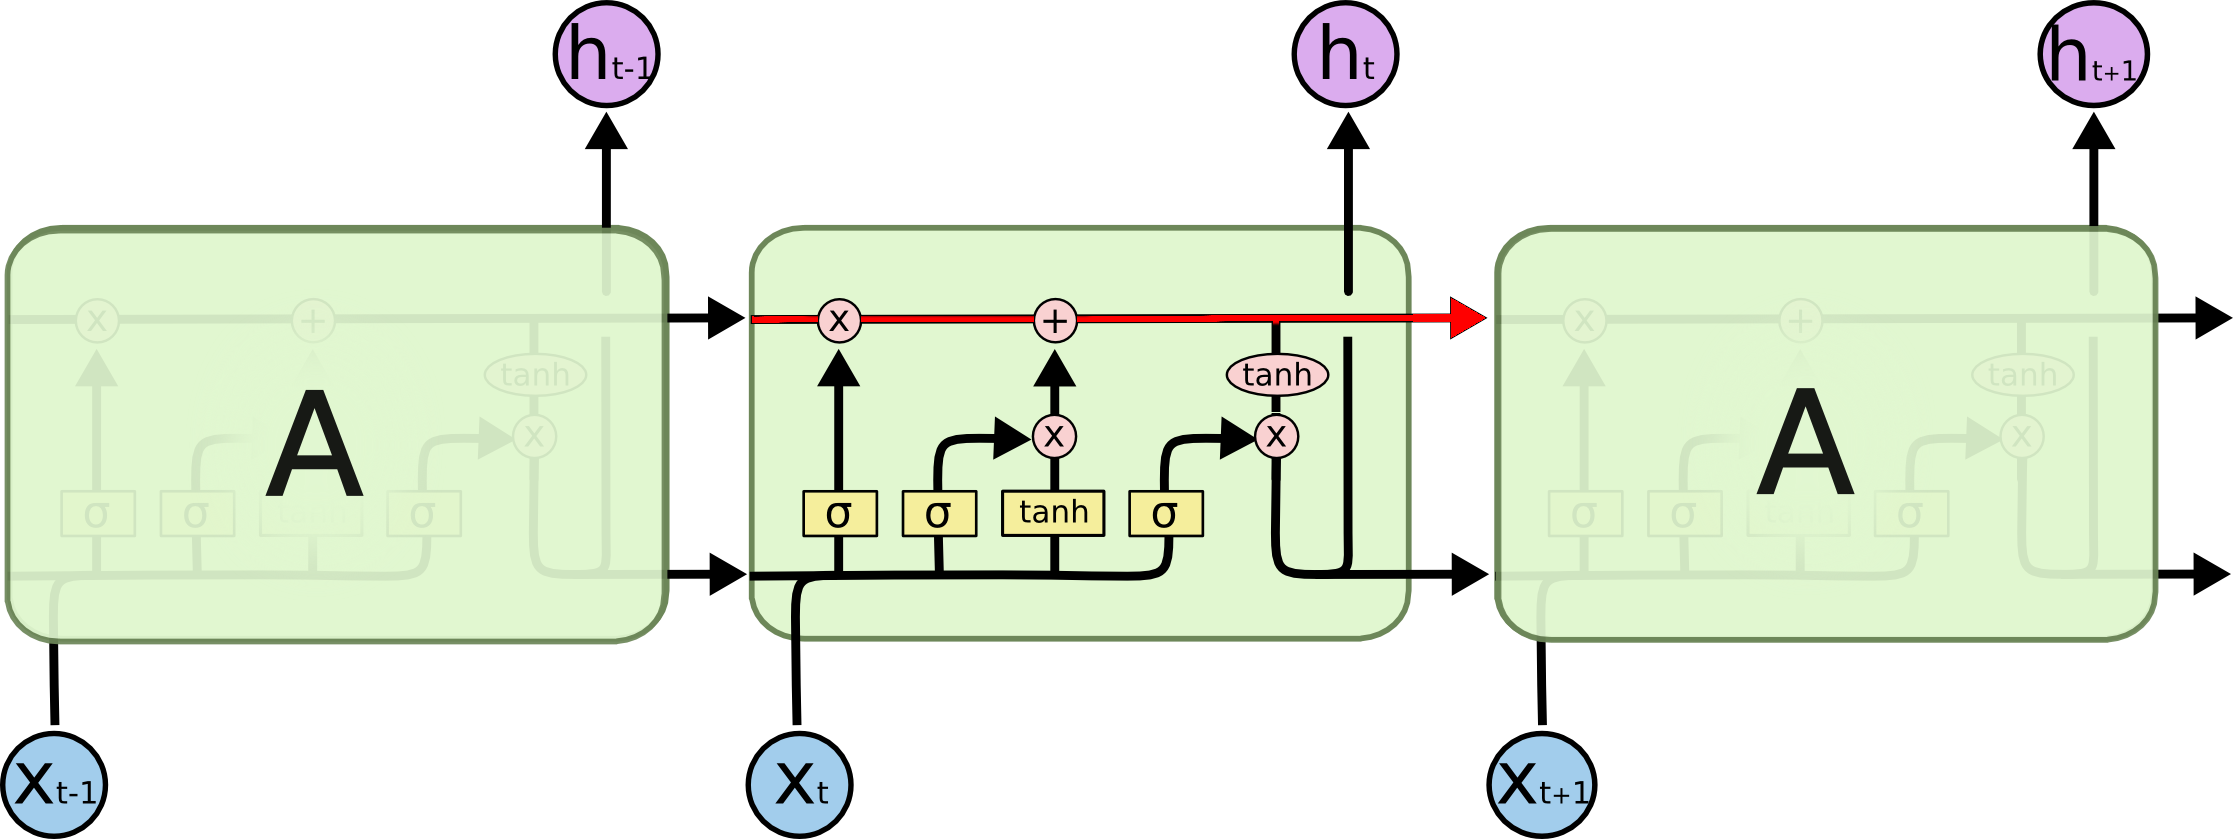
\includegraphics[width=5in]{lstm-chain}
\caption{An LSTM-block showing gated flow of information in red color}\label{fig:lstm-chain}
{Source: \href{http://colah.github.io/posts/2015-08-Understanding-LSTMs/}{http://colah.github.io}\hfill}
\end{figure}


\subsection{ResNet}

ResNet\autocite{he2016deep}\autocite{he2016identity} is the winner of ILSVRC 2015.
ResNet extends the concept of highway in a more simpler way by just adding input every two layers,
it's like having constant \(T=0.5\) in formula \ref{eq:highway}.

The main idea as in figure {fig:resnet} from first paper\autocite{he2016deep} is to pass the original signal ``as is''
after every two layers with trainable weights using addition and ``ReLU'' (as seen in figure \ref{fig:resnet-block})
then just stack this building unit deeper and deeper.

\begin{figure}[!h]
\centering
    \begin{subfigure}[b]{0.4\textwidth}
        \includegraphics[width=\textwidth]{resnet}
        \caption{ResNet Building Block}\label{fig:resnet-block}
    \end{subfigure}
    \begin{subfigure}[b]{0.4\textwidth}
        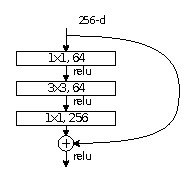
\includegraphics[width=\textwidth]{resnet-bottleneck}
        \caption{ResNet Bottleneck}\label{fig:resnet-bottleneck}
    \end{subfigure}
\caption{ResNet building block}\label{fig:resnet}
{Source: \autocite{he2016deep}\hfill}
\end{figure}

This paper use a form of separable operator reduction called ``bottleneck'' (as in figure \ref{fig:resnet-bottleneck})
which places 1×1 kernel before and after 3×3 kernel.

The second paper\autocite{he2016identity} changes the placement of batch normalization and ReLU as seen in figure \ref{fig:resnet-bn}

And because the original signal is not fading with depth this allowed them to go deeper up to one thousand layers.
Different variation of this design have 50, 101, 152, 200, and even 1000 layers.

ResNet uses 7×7 convolutions with stride of 2, pool 3×3/2 then just repeat the building block of [1×1, 3×3, 1×1 ] many times,
the last 1×1 output volume is 1×1×1000 and it’s followed by average pooling from 2000 to 1000
then fully connected layer to classes.

And like inception, ResNet does not have a layer with most weights,
the weight is well distributed as the heaviest layer in terms of number of parameters
have about 8\% of weights in the 50-layer version (that is the last fully connected layer),
4.7\% in the 101 layer version, 3.9\% in the 151 layers version.

And like inception number of layers is misleading because the use of separable operators.

\begin{figure}[!h]
\centering
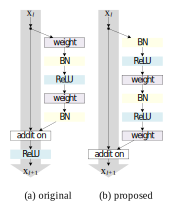
\includegraphics[width=0.48\textwidth]{resnet-bn}
\caption{Placement of Batch normalization in ResNet}\label{fig:resnet-bn}
{Source: \autocite{he2016identity}\hfill}
\end{figure}


\subsection{Inception v4 And Inception-ResNet}

Inception v4 And Inception-ResNet\autocite{szegedy2017inception} are variations of previously discussed Inception
that utilized residual connections in a way similar to ResNet\autocite{he2016deep}

\subsection{DenseNet}
Densely connected convolutional networks (DenseNet)\autocite{huang2016densely},
to counter vanishing gradients as network becomes deeper,
a way for first input is allowed to pass through to deeper layers,
Highway Networks which gates input and optionally pass it to deeper layers
and ResNet which adds input every two layers/blocks,
DenseNet just concatenate signals for all previous layers as in figure \ref{fig:densenet}.

\begin{figure}[!h]
\centering
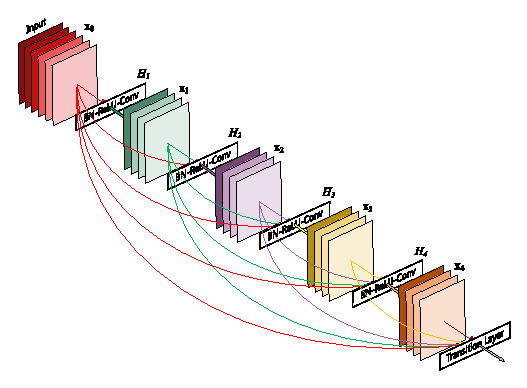
\includegraphics[width=3in]{densenet}
\caption{DenseNet have each layer gets input from all previous layers}\label{fig:densenet}
{Source: \autocite{huang2016densely}\hfill}
\end{figure}


\subsection{MobileNet and SqueezeNet}

MobileNet\autocite{howard2017mobilenets} does not compete on accuracy but on speed.
Similar to SqueezeNet\autocite{iandola2016squeezenet} in the use of the following strategies\autocite{iandola2016squeezenet}\autocite{he2015convolutional}:
Delay down-sampling toward the end of the network,
that is pooling layers and convolutions with strides to get accuracy
which other network put early in the network to reduce number of operations.
Instead they use \(1\times 1\) convolutions instead of more larger \(3\times 3\) 
and reduce the depth of the \(3 \times 3\) filters to reduce number of parameters and operations.

The idea of \(1\times 1\) did not first appear with MobileNet and SqueezeNet,
as it's used heavily in Inception as seen before,
but in MobileNet it's used as replacement of earlier stride to reduce the network computational cost,
MobileNet v1.0 has competitive accuracy compared with inception v1 with half number of parameters.
MobileNet v2.0\autocite{sandler2018inverted} reaches better accuracy than Inception v1 with half the number of parameters.

There are no fully connected layer in SqueezeNet, which is called ``Quantizing FC layer''\autocite{wu2016quantized}.

\subsection{NASNet}

NASNet\autocite{zoph2017learning} has multiple settings, some are small suitable for
mobile applications that competes with MobileNet and Inception v1.
While others has order of magnitude more operations and weights that compete with Inception v4 and ResNet in terms of accuracy. 
Here are two interesting settings on NASNet:

\begin{itemize}
\item NASNet-A (6 @ 4032), 331x331, 88.9M params, 23.8B mults
\item NASNet-A (4 @ 1056), 224x224, 5.3M params, 564M mults
\end{itemize}

The main contribution of NASNet is not their specific network design,
but rather is having that design done by a neural network instead of a human expert.
Another aspect of it, that the training did not happen on ImageNet high resolution images of 1K classes
but rather on a simpler task of classifying tiny images of ten classes (CIFAR-10),
then the architecture is transferred to ImageNet 1k.

\section{Pre-processing}

The bare minimum pre-processing is to resize input image to make it
fit the perceptive field of the network (typically \(224\times 224\) pixels).
Some CNNs have special normalization done to input images,
like subtracting image mean as in VGG\autocite{simonyan2014very},
while others also divide by the standard deviation of the image.
Such transformations should be done in both training phase and prediction phase.

Some pre-processing is done in training phase only to have better generalization, like:
random cropping of a random bounding box in input image, 
random left/right flipping, and random color distorting (brightness, saturation, and contrast).

\section{Stochastic Optimizers}

The factors that affect the efficiency of ANN have been discussed in academia for ages
for example \autocite{lecuniefficient}
(which was part of a book published 1998\autocite{orr1998neural}, that has more recent editions \autocite{orr2012neural}).

There are variations of plain stochastic gradient descent (SDG), the are adaptive and faster to converge like:
SGD momentum\autocite{sutskever2013importance},
Adagrad\autocite{duchi2011adaptive},
Adam\autocite{kingma2014adam},
Adadelta\autocite{zeiler2012adadelta},
and RMSprop\autocite{dozat2016incorporating}\autocite{sutskever2013importance}

PhD. student Sebastian Ruder has made a nice \href{http://sebastianruder.com/optimizing-gradient-descent/}{animation} that compare how they work.

\section{Knowledge Transfer and fine-tuning}

Humans learn multiple tasks at once, and they learn how to generalize,
and how to learn and the learning process is non-stopping continuous streams.
If a computer program that work on a family of tasks each having its own training and
its own experience and its own performance measures, then the computer program is said\autocite{thrun1998learning}
to be capable of ``learning to learn'' if its performance depends on number of tasks (not just a single task).
This field is called multi-task learning and in this type both tasks are trained simultaneously and
one of them enhances the other.

\begin{figure}[!h]
\centering
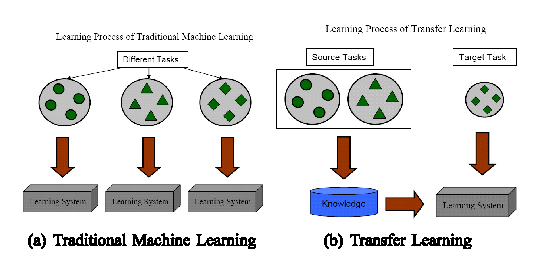
\includegraphics[width=5in]{transfer-learning}
\caption{Transfer-learning}\label{fig:transfer-learning}
{Source: \autocite{pan2010survey}\hfill}
\end{figure}

``Self-taught Learning'' as in \autocite{raina2007self} use unsupervised machine learning to train the machine
how to generalize and construct higher-level features despite the lack of labeled dataset in source task,
and utilize that to in the labeled supervised target task.

Knowledge Transfer is all about reusing some parts from an already solved task and
borrowing knowledge from an already trained and accurate classifier as seen in figure \ref{fig:transfer-learning}.
There are several settings for such process\autocite{pan2010survey} depending on the relation between
source domain \( D_{s} \) and target domain \( D_{t} \), and the relation between
source task \( \tau_{s} \) and target task \( \tau_{t} \) as they can be either the same or similar but different.
Also Knowledge Transfer has to define\autocite{pan2010survey}

\begin{itemize}
\item ``What to transfer?''
\item ``How to transfer?''
\item ``When not to transfer?''
\end{itemize}

The transfer algorithm has to find what parts of knowledge can be transferred across domains and tasks,
then how to actually do the transfer, depending on the availability of labeled training
dataset in either of the domains (source and target).
Domain adaptation\autocite{saenko2010adapting} considered same task on two different but similar domains,
by finding a cross-domain transformation that maps points in source domain to target domain,
as opposed to ``Category Transfer'' which maps labels as in figure \ref{fig:domain-adapt}.

% \autocite{pratt1993discriminability}

\begin{figure}[!h]
\centering
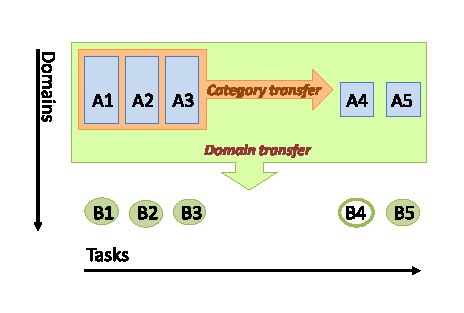
\includegraphics[width=2in]{domain-adapt}
\caption{Difference between ``Category Transfer'' and ``Domain Transfer''.}\label{fig:domain-adapt}
{Source: \autocite{saenko2010adapting}\hfill}
\end{figure}

There are several categorization for the ``how''\autocite{pan2010survey}:

\begin{description}
\item [Instance-transfer] To re-weight some labeled data in the source domain for use in the target domain.
\item [Feature-representation-transfer] To find a ``good'' feature representation that reduces difference between the source and the target
domains and the error of classification and regression models.
\item [Parameter-transfer] Discover shared parameters or priors between the source domain and target domain models, which can benefit for transfer learning
\item [Relational-knowledge-transfer] Build mapping of relational knowledge between the source domain and the target domains. Both domains are relational domains and i.i.d assumption is relaxed in each domain.
\item [Architecture transfer] train an \gls{rnn} to find best architecture on a simple task, transfer architecture to difficult task as in NASNet\autocite{zoph2017learning}
\end{description}

% TODO: do we need to talk about meta learner / fast-learner. 

Other types of transfer learning have a prior (not simultaneous) knowledge (that is possibly static)
in one task that is used to induce knowledge in another task both in same domain and feature space
which is the type that this research would focus on where source domain and target domain are the same
(which is the input image and its pixels are the feature).
Source task is the ImageNet classification task from \gls{ilsvrc},
and the prior knowledge is one of the pre-trained state-of-the-art models.
Target task is to classify different dataset obtained from the e-Commerce platform or the fine-grained datasets of flowers,
dogs, birds, food.

Fine-tuning\autocite{zeng2016gated}\autocite{ouyang2016factors}\autocite{sharif2014cnn} is a type of ``Parameter-transfer''.
Taking an ``off-the-shelf''\autocite{sharif2014cnn} pre-trained state of the art \gls{cnn} model
then re-fit it on different task by taking all weights except those in last fully connected layer 
or by adding an \gls{svm} after last convolution (called CNN-SVM).
This works because several researches\autocite{donahue2014decaf}\autocite{girshick2014rich}\autocite{oquab2014learning}
have shown and even visualized\autocite{zeiler2014visualizing} that when moving toward the end of the neural network,
the deeper the more high-level features, moving from low primitives to complete objects or entities (eyes, faces, ..etc.)

% off-topic \autocite{taigman2014deepface}, \autocite{toshev2014deeppose}, \autocite{zhang2014panda}

Some other methods utilize knowledge from unlabeled datasets or noisy datasets
and transfer knowledge to enhancing labeled but small dataset as in papers\autocite{reed2014training}\autocite{sukhbaatar2014training}\autocite{sukhbaatar2014learning}\autocite{van2015building}

A different approach was done by Google Brain Team in their paper \autocite{bello2017neural}
as they proposed a way for ``Architecture Search''
but that was expensive for large database, that's why in their other paper\autocite{zoph2017learning}
used transferred knowledge from a very simple problem that is CIFAR-10 dataset to
the state-of-the-art difficult problem ImageNet\autocite{deng2009imagenet} dataset.
They did not transfer weights, as they train from scratch after transfer,
they transfer architecture and design not knowledge which resulted in NASNet discussed before.


\chapter{Implementation}

\section{Preparing datasets}

\subsection{Stock Datasets}

There are many stock datasets in literature used to study image recognition techniques, like
\textbf{``Oxford 102 Flowers Dataset''}\autocite{nilsback2008automated},
\textbf{``The Caltech-UCSD Birds-200-2011 Dataset''}\autocite{WahCUB_200_2011}
and \textbf{``The Oxford-IIIT Pet Dataset''}\autocite{parkhi12a} which have 37 species of cats and dogs.
For short, those datasets are called flowers-102, birds-200, and pets-35 respectively.

For toy problems, a much simpler datasets with smaller number of classes are needed.
That's why such datasets were crafted by manipulating previously mentioned datasets.
For example, two classes dataset of ``Cats and Dogs'' was created by adapting pets-37 dataset, merging 12 cats breeds into a ``Cats'' class, and the rest are merged into ``Dogs'' class.
A dataset with three classes ``Cat, Dog or Bird''
was created by merging all pictures from birds-200 dataset into one class
(taking random 3,000 pictures out of around 11,000 pictures),
then add them to the previous ``Cats and Dogs'' dataset.

Another toy dataset is \href{http://download.tensorflow.org/example_images/flower_photos.tgz}{the five flowers dataset}(flowers-5)
containing labeled images for Daisy, Dandelion, Roses, Sunflowers, and Tulips.

\subsection{Vehicle Viewing Angles Dataset}

For the sake of cleaning car images, a small hand-picked dataset was created to identify vehicle viewing angles into nine classes, 

\begin{description}
\item [interior dashboard view], having either steering wheel or odometer visible.
\item [interior seats view] no steering wheel visible nor odometer visible.
\item [front view] both head lights are visible, no doors are visible.
\item [back view] both tail lights are visible, no doors are visible.
\item [side view] both front door and back door visible, both side wheels are visible,
at most one head light visible and at most one tail light visible (if half of radiator grille is visible, then it's front-side view)
\item [front-side view] both front door and back door visible, both side wheels are visible, and both front head lights are visible (or more than half of the radiator grille)
\item [back-side view] both front door and back door visible, both side wheels are visible, and both back tail lights are visible
\item [Wheels] pictures of cars with only one wheel is visible and no-car wheels and alloy wheel.
\item [under-hood]  without headlights or grill visible
\end{description}

Another dataset is created by subdividing each of ``Side view'', ``Back view'', and ``Back-side view'' into six classes:
Sedan, Coupe, Station, Hatchback, SUV, and Pickup or truck.

Those two datasets are hand-picked from various websites, google image search, wikipedia,
and \href{http://opensooq.com}{OpenSooq.com}, to have about 200 image from each class.
Making sure to have different backgrounds, various brands, various models, designs of modern and legacy vehicles
both stock ``staged'' images and natural images.

\subsection{Noisy Vehicle Make-Model-Year Dataset}

\href{http://opensooq.com}{OpenSooq.com} is the leading market place in the middle-east,
having thousands of vehicles for sale added by their owners every day.
Owners upload many pictures of their cars and tag them with make/model/year
among other details (like mileage, transmission, ...etc.).
Opensooq have tons of labeled images. But those user-generated images are noisy,
as they have pictures of registration papers, insurance papers,
inspection papers (local or CarFax), maintenance history, picture of business cards, dealer logos, ..etc.
Beside non-car pictures, sellers upload pictures showing some selling points
like moon roof, leather seats, door lock pin, large wheels size, alloy wheels, under the hood customization.
Those picture (as in figure \ref{fig:noisy}) have no association with any of the desired labels.
Such pictures are important to the seller, but from the point of having pictures that conclude tags like car make and model
those pictures are merely noise.

\begin{figure}[!h]
\centering
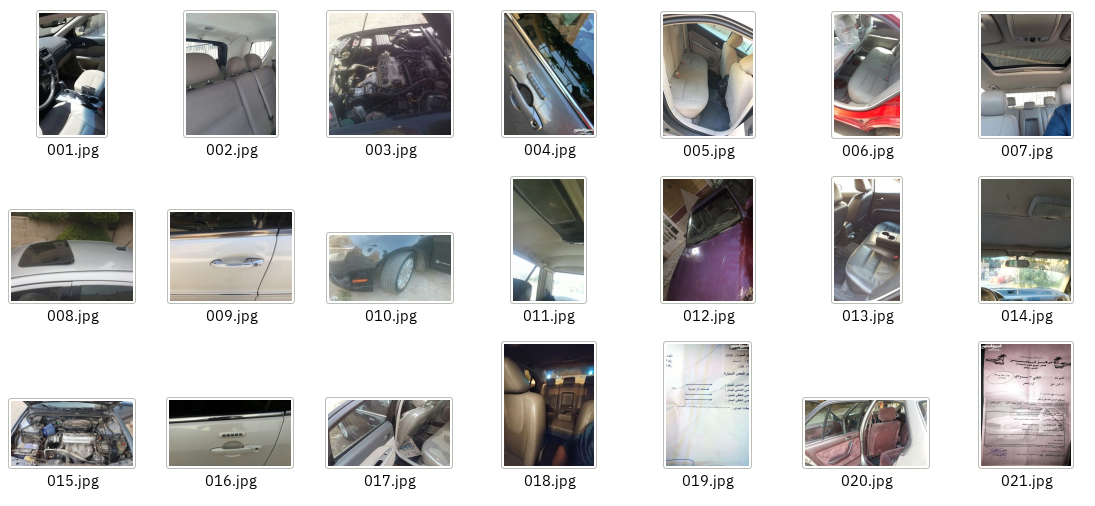
\includegraphics[width=\textwidth]{noisy}
\caption{Examples of inconclusive pictures uploaded by sellers}\label{fig:noisy}
\end{figure}

\href{http://opensooq.com}{OpenSooq.com} have generously provided us with hundreds of thousands of pictures of each class.

\begin{itemize}
\item 76 distinct car make
\item more than 1600 classes of make-model
\item more than 20 thousand class of make-model-year
\end{itemize}

Many of 20 thousand classes are distinct only on paper, many of them look similar and should be grouped together
For example, Volkswagen Golf Mk3 looked the same from 1991 to 2002, and Beetle looked almost the same since 1956
as seen in figure \ref{fig:beetle}.
This means that this dataset need a lot of cleanup that is discussed later.

A cleaned dataset was produced based on this dataset, that is discussed in later sections.

\begin{figure}[!htbp]
\centering
    \begin{subfigure}[t]{0.48\textwidth}
        \centering
        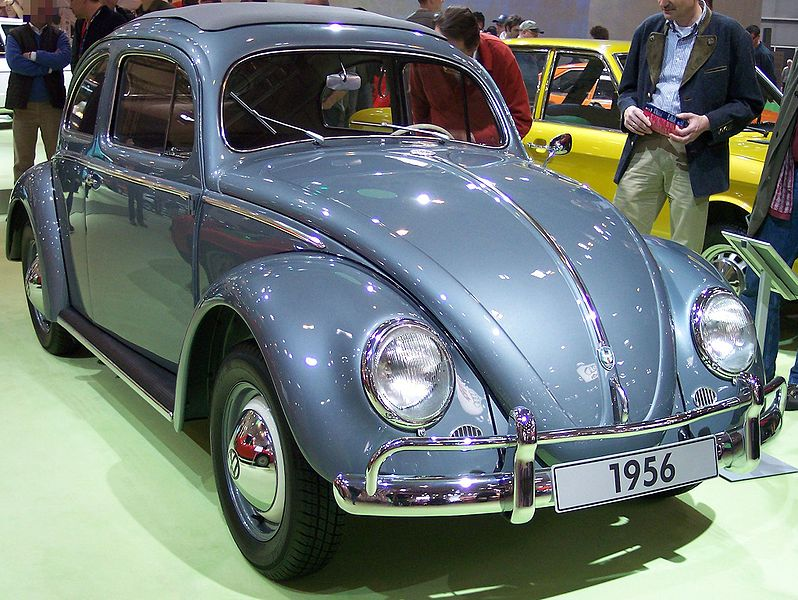
\includegraphics[width=\textwidth]{beetle-1956}
        \caption{Original look of Volkswagen Beetle in 1956}
    \end{subfigure}
    \begin{subfigure}[t]{0.48\textwidth}
        \centering
        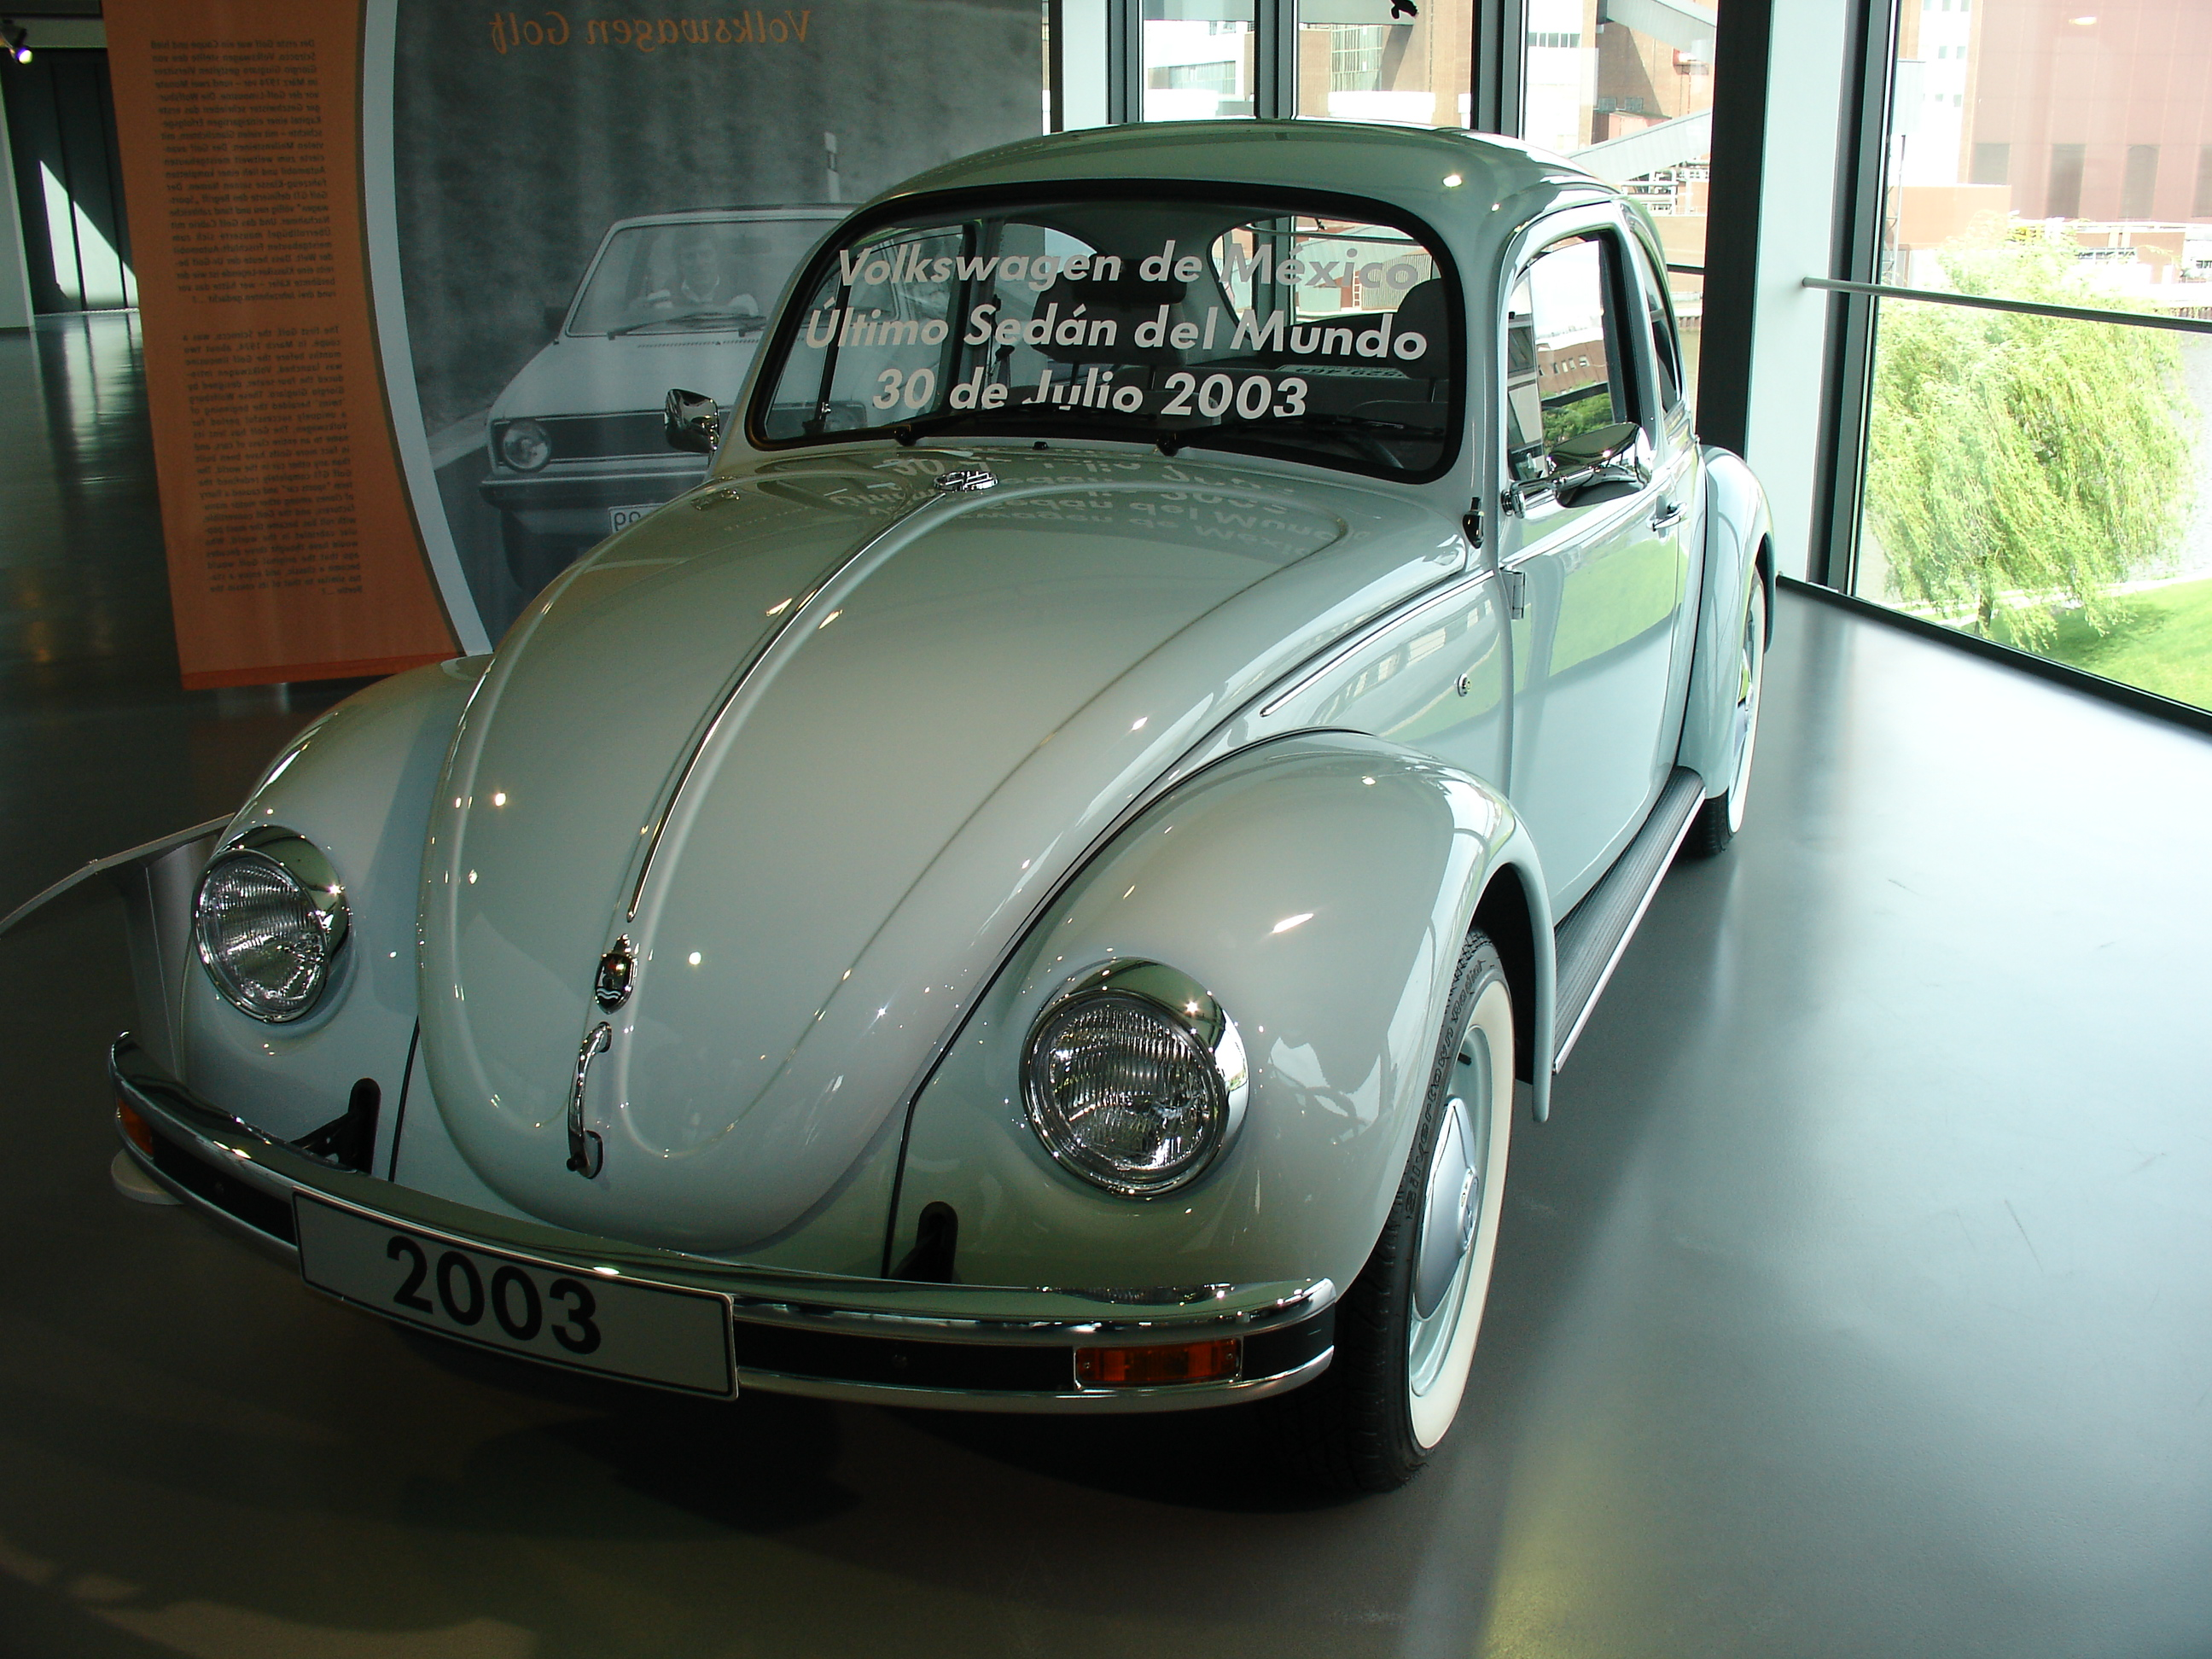
\includegraphics[width=\textwidth]{beetle-2003}
        \caption{A Type 1 VW Beetle produced in 2003 Puebla, Mexico known as ``Última Edición''}
    \end{subfigure}
    \begin{subfigure}[b]{\textwidth}
        \centering
        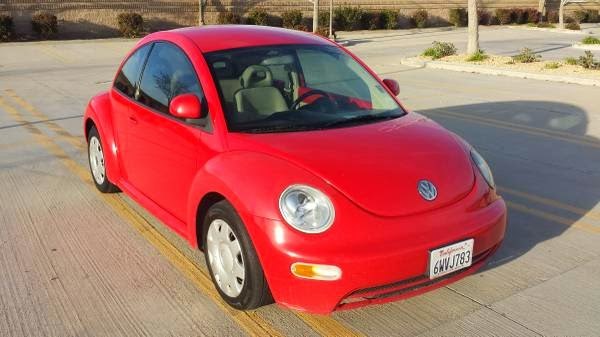
\includegraphics[width=\textwidth]{beetle-new-1998}
        \caption{The look of VW new beetle in 1998}
    \end{subfigure}
\caption{Different models of VM beetle}\label{fig:beetle}
\end{figure}

\subsection{Pre-processing Images}

while most CNNs take input of size \(224\times224\),
most datasets have images of varying sizes,
mostly too large images (full HD images or better) as they were scraped from social media or quality websites.
It would be a waste of resources to store and photos of such large sizes.

To unify sizes and make it more suitable to such CNNs,
All images have been re-sized keeping aspect ratio so that it would be at most \(300\times300\)
using the following command from \href{https://www.imagemagick.org/}{ImageMagick Suite}

\begin{verbatim}
$ convert input.jpg -resize 300x300'>' output.jpg
\end{verbatim}

% find opensooq_photos/ -type d | while read a; do mkdir -p "2$a" 2>/dev/null ; done
% find opensooq_photos/ -type f | while read a; do convert "$a" -resize 400x400'>' "2${a/.png/.jpg}" ; done

This is one time job that done once beside different run-time pre-processing done by different CNNs.

\section{Tools}

\begin{itemize}
\item SciKit Learn
\item TensorFlow
\item TensorFlow slim models
\end{itemize}

\section{Procedures}

\subsection{Failure of reduction via pre-processing before CNN}

One of the initial ideas was the use of some pre-processing techniques to 
make input images into sparse ``points of interest'' or ``key points''.
By focusing on smaller number of points,
hoping to get a simpler problem that would require less resources.
Hand crafted ``hit-or-miss'' convolution filters was used
(hits are ones over their count, and misses are minus ones over their count).
One of them those filters was corner filter (in figure \ref{fig:hmt-corner}) which should be applied
in its four variations (rotated 90° each).
Another tried was done using a small empty circle ``hit-or-miss'' (shown in figure \ref{fig:hmt-circle}).
Those were applied to input images then taking local peaks (using ``skimage.feature.peak\_local\_max()'').
The results were comparable to Harris corner filter.

The idea was to make input images sparse to reduce the problem before feeding input images to ANN
hoping to get a simpler problem that would require smaller resources to train.
But ANN takes fixed-sized input or sequences in case on RNN.
That's why the searcher could not make any use of the reduction and
moved to reusing off-the-shelf pre-trained CNN.

\begin{figure}[!htbp]
\centering
    \begin{subfigure}[t]{0.32\textwidth}
        \centering
\[
\frac{1}{3} \cdot
\begin{bmatrix}
0 & +1 & 0 \\
-1 & +1 & +1 \\
-1 & -1 & 0 
\end{bmatrix}
\]
    \end{subfigure}
    \begin{subfigure}[b]{0.65\textwidth}
        \centering
        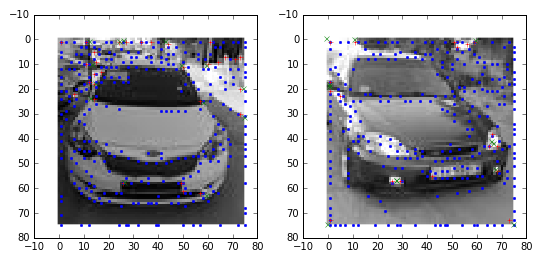
\includegraphics[width=\textwidth]{hmt-4-corners}
    \end{subfigure}
\caption{Corner hit-or-miss transform convolutional matrix on left, results in blue compared to Harris corner in red}\label{fig:hmt-corner}
\end{figure}

\begin{figure}[!htbp]
\centering
    \begin{subfigure}[b]{0.32\textwidth}
        \centering
\[
\begin{bmatrix}
-\frac{1}{4} & \frac{1}{12} & \frac{1}{12} & \frac{1}{12} & -\frac{1}{4} \\
\frac{1}{12} & 0 & 0 & 0 & \frac{1}{12} \\
\frac{1}{12} & 0 & 0 & 0 & \frac{1}{12} \\
\frac{1}{12} & 0 & 0 & 0 & \frac{1}{12} \\
-\frac{1}{4} & \frac{1}{12} & \frac{1}{12} & \frac{1}{12} & -\frac{1}{4}
\end{bmatrix}
\]
    \end{subfigure}
    \begin{subfigure}[b]{0.65\textwidth}
        \centering
        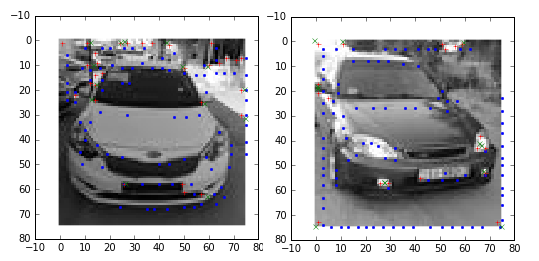
\includegraphics[width=\textwidth]{hmt-small-circle}
    \end{subfigure}
\caption{Small circle hit-or-miss transform convolutional matrix on left, results in blue}\label{fig:hmt-circle}
\end{figure}

\subsection{Category Adaptation}

Category Adaptation works by finding mapping between 
any of state-of-the-art pre-trained off-the-shelf models
(like \href{http://www.image-net.org/challenges/LSVRC/2012/}{ILSVRC-2012-CLS} winners).
For e-commerce like \href{http://opensooq.com}{OpenSooq.com} 
instead of training a model to identify cars, electronics, ...etc.
one can just map the one thousand ImageNet classes into his/her own classes as in table \ref{table:mapping_os_imagenet},
and flag non-mapped images for human moderation.

Human effort needed to carefully map the one thousand class to relevant categories
is much less than preparing a clear dataset suitable for training.

Passing noisy labeled dataset and taking top most classes (using percentiles) is important in both validating human mappings
and in finding unusual flaws in ImageNet,
for example, images of car inspection papers usually get detected as ``restaurant menu'' or ``website''
and pictures showing car seats might get identified as ``barber chair'' or ``stretcher''.

The benefit of ``Category Adaptation'' that it does not require training nor preparing dataset.
On the other hand, it can't get fine-grained, as you can merge categories but you can't divide them,
for example you can not identify different vehicle types (Sedan, Hatchback, SUV, ...etc.), makers, models.
You can't add new categories, for example smart phones might be detected as modems or other older devices that
were part of \href{http://www.image-net.org/challenges/LSVRC/2012/}{ILSVRC-2012-CLS} database\autocite{deng2012imagenet}.

\begin{table*}\caption{Example of ``Category Adaptation'' hand-picked mapping of ImageNet classes to some of OpenSooq e-Commerce Categories}\label{table:mapping_os_imagenet}
\begin{tabularx}{\textwidth}{lX}
\toprule
OpenSooq Label & ImageNet Label \\
\midrule
\multirow{14}{*}{Autos} & beach wagon \\
 & minivan \\
 & jeep \\
 & limousine \\
 & convertible \\
 & pickup \\
 & minibus \\
 & sports car \\
 & tow truck \\
 & ambulance \\
 & cab \\
 & racer \\
\midrule
\multirow{12}{*}{Electronics} & cellular telephone, cellphone, mobile phone \\
 & desktop computer \\
 & dishwasher, dish washer, dishwashing machine \\
 & joystick \\
 & laptop, laptop computer \\
 & modem \\
 & printer \\
 & refrigerator, icebox \\
 & remote control, remote \\
 & television, television system \\
 & vacuum, vacuum cleaner \\
 & washer, automatic washer, washing machine \\
\bottomrule
\end{tabularx}
\end{table*}

\subsection{Understanding Weights}

In case of usual ANN, the last layer (the fully connected layer) takes features and multiply them with weights matrix
(\(n\times m\) matrix where \(n\) is number of input features, and \(m\) is number of classes),
add bias and then apply the activation function, then apply ``softmax()'' to convert them to probability like results.
Some CNN have that usual ANN fully connected layer as last layer while others have an equivalent \(1\times1\) convolution
of depth \(m\). In both cases we can have a weights matrix of size \(n\times m\).
As in equation \ref{eq:ann_weights} we can look
to the weights matrix as if it's composed of \(m\) vectors \(\vec{v}_i\) in feature space of dimension \(n\).
Each vector \(\hat{v}_i\) represent the direction of that class, and
the magnitude of the vector is used to control the probability when two classes are activated by same features.

\begin{equation}
W_{n\times m} =
\begin{bmatrix}
w_{11} & w_{12} & \cdots  &  w_{1m} \\
w_{21} & w_{22} & \cdots  &  w_{2m} \\
\vdots  & \vdots  & \ddots  &  \vdots  \\
w_{n1} & w_{n2} & \cdots  &  w_{nm}
\end{bmatrix}
=
\begin{bmatrix}
\vec{v}_{1} & \vec{v}_{2} & \cdots & \vec{v}_{m}
\end{bmatrix}
\label{eq:ann_weights}
\end{equation}

\subsection{Using Category Adaptation to Cleanup Dataset}

As mentioned before \href{http://opensooq.com}{OpenSooq.com} provided the researcher with
a ``Noisy Vehicle Make-Model-Year Dataset''.
``Category Adaptation'' was used to clean this dataset by removing non-cars pictures from it.

A tool named ``img-grep'' that is inspired by UNIX philosophy
and \href{http://pubs.opengroup.org/onlinepubs/009695399/utilities/grep.html}{UNIX grep utility} was created .
This tool reads image file names from standard input,
and output only matching file names (or non-matching if --exclude is passed).
The matching criteria is either a list of label indices or a file containing such label indices. 

Using mapping as in table \ref{table:mapping_os_imagenet}, non-car images were removed from dataset,
surprisingly more 20\% of images were removed, which is understandable because on average a car post have 5 images
one of them is a picture of some papers (registration/inspection).

\begin{program}
\begin{verbatim}
#! /bin/bash
find src -type f -name '*.jpg' | \
  img-grep --model_dir inception_v1 \
    --idx 437,657,610,628,512,718,655,818,865,408,469,752 |
  while read filename
  do
    cp "${filename}" "${filename/src/dst}"
  done
\end{verbatim}
\caption{A simple bash script that uses ``img-grep'' to create a cleaned up version of dataset}
\end{program}


\subsection{Category Adaptation using weights manipulations}

One can produce cars vs. electronics using category adaptation
by mapping classes of the results as in table \ref{table:mapping_os_imagenet}.
One might consider doing this by simply averaging vectors of source classes to be merged in one target class

\begin{equation}
\vec{v}_{t} = ( \vec{v}_1+\vec{v}_2+\ldots+\vec{v}_k ) / k
\label{eq:cat_adapt_avg}
\end{equation}

or even better using unit vectors adjusted by its probability in target task \(p_i\)
and the result vector magnitude is set to be the average magnitude in source task
if we are constructing a target model from scratch or the average magnitude in acceptor model
in case of knowledge transfer to an existing target model.

\begin{equation}
\vec{v'}_{t} = \frac{ \sum\nolimits_{i} p_{i}\hat{v}_i }{ \sum\nolimits_{i} p_{i} }
\label{eq:vec_cat_adapt}
\end{equation}
\begin{equation}
\vec{v}_{t} = \bar{V} \hat{v'}_{t}
\label{eq:vec_cat_adapt2}
\end{equation}


\subsection{Application on ``Cats, Dogs and Birds'' dataset}

As discussed before\ref{eq:ann_weights} the weights matrix is composed of vectors in feature space,
one can use a formula to \ref{eq:vec_cat_adapt} create weights.
A small number of pictures were passed from ``Cats, Dogs, and Birds'' dataset,
exactly 100 pictures (out of thousands) from each of the three classes to Inception v1 pre-trained on ImageNet
to find probability of donor class in target class and got results as in table \ref{table:inception_cats}.

\begin{table*}\caption{Results of passing some cats, dogs and birds pictures to ImageNet Inception v1}\label{table:inception_cats}
\begin{adjustwidth}{-2in}{-2in} %
\centering
\begin{tabular}{@{}lrl@{}}
\toprule
Target Class & Probability \(p_i\) & Donor Model Class \\
\midrule
\multirow{3}{*}{Cat} & 49\% & 286:Egyptian cat \\
 & 19\% & 285:Siamese cat \\
 & 10\% & 284:Persian cat \\
 & 10\% & 282:tabby cat \\
 & 2\% & 288:lynx, catamount \\
\midrule
\multirow{9}{*}{Dog} & 14\% & 181:pit bull terrier \\
 & 10\% & 243:boxer \\
 & 8\% & 213:English setter \\
 & 5\% & 211:German short-haired pointer \\
 & 5\% & 200:Scotch terrier \\
 & 4\% & 262:keeshond \\
 & 4\% & 259:Samoyed \\
 & 4\% & 256:Leonberg \\
 & 3\% & 258:Great Pyrenees \\
 & 3\% & 248:Saint Bernard \\
 & 3\% & 238:miniature pinscher \\
 & 3\% & 203:soft-coated wheaten terrier \\
 & 3\% & 188:Yorkshire terrier \\
 & 3\% & 163:beagle \\
 & 2\% & 274:Canis dingo \\
 & 2\% & 264:Pembroke \\
 & 2\% & 257:Newfoundland dog \\
 & 2\% & 220:cocker spaniel \\
 & 2\% & 158:papillon \\
 & 2\% & 154:Maltese dog \\
\midrule
\multirow{9}{*}{Bird} & 10\% & 11:brambling \\
 & 9\% & 17:bulbul \\
 & 9\% & 13:linnet \\
 & 6\% & 147:albatross, mollymawk \\
 & 6\% & 12:goldfinch, Carduelis carduelis \\
 & 5\% & 20:chickadee \\
 & 5\% & 19:magpie \\
 & 5\% & 18:jay \\
 & 4\% & 96:jacamar \\
 & 4\% & 144:oystercatcher \\
 & 4\% & 14:snowbird \\
 & 3\% & 95:hummingbird \\
 & 3\% & 22:kite \\
 & 3\% & 16:Turdus migratorius \\
 & 2\% & 93:bee eater \\
 & 2\% & 92:coucal \\
 & 2\% & 21:water ouzel \\
 & 2\% & 15:indigo bird \\
 & 2\% & 134:bittern \\
 & 2\% & 129:black stork \\
\bottomrule
\end{tabular}
\end{adjustwidth}


\end{table*}

\subsection{Fine Tuning off-the-shelf models}

Fine-Tuning an already trained model work by reconstructing a new ANN,
transferring weights from the pre-trained network (called donor model or source model)
to the newly constructed one (called acceptor or target model)
up to some point as seen in figure \ref{fig:ann4}.

Weights transferred from the donor model carries already learned knowledge on how to extract features and
how to pre-process them\autocite{oquab2014learning}.
On the other hand, weights left to be trained are the decision making parts (decision making layer),
which is not transferred but left to be trained on target task which might be different than source task.

The same thing with ConvNets as seen in figure \ref{fig:cnn-doner-acceptor},
as they typically have some fully connected layers (just like usual ANN) toward the end,
or have an equivalent 1x1 convolution that act as a fully connected ANN layer,
that leads to the classes after being passed to softmax function.

Fine-tuning an existing model gives state-of-art accuracy\autocite{ouyang2016factors}
with fraction of training time (compared to fully train the new model)
as millions of weights are transferred from the donor model without training.


If training one layer was not enough to get the desired accuracy,
one might add more fully connected layers toward the end of the network
or include more layers in the trainable parts (blue colored layers in figure \ref{fig:ann4}).

\begin{figure}[!h]
\centering
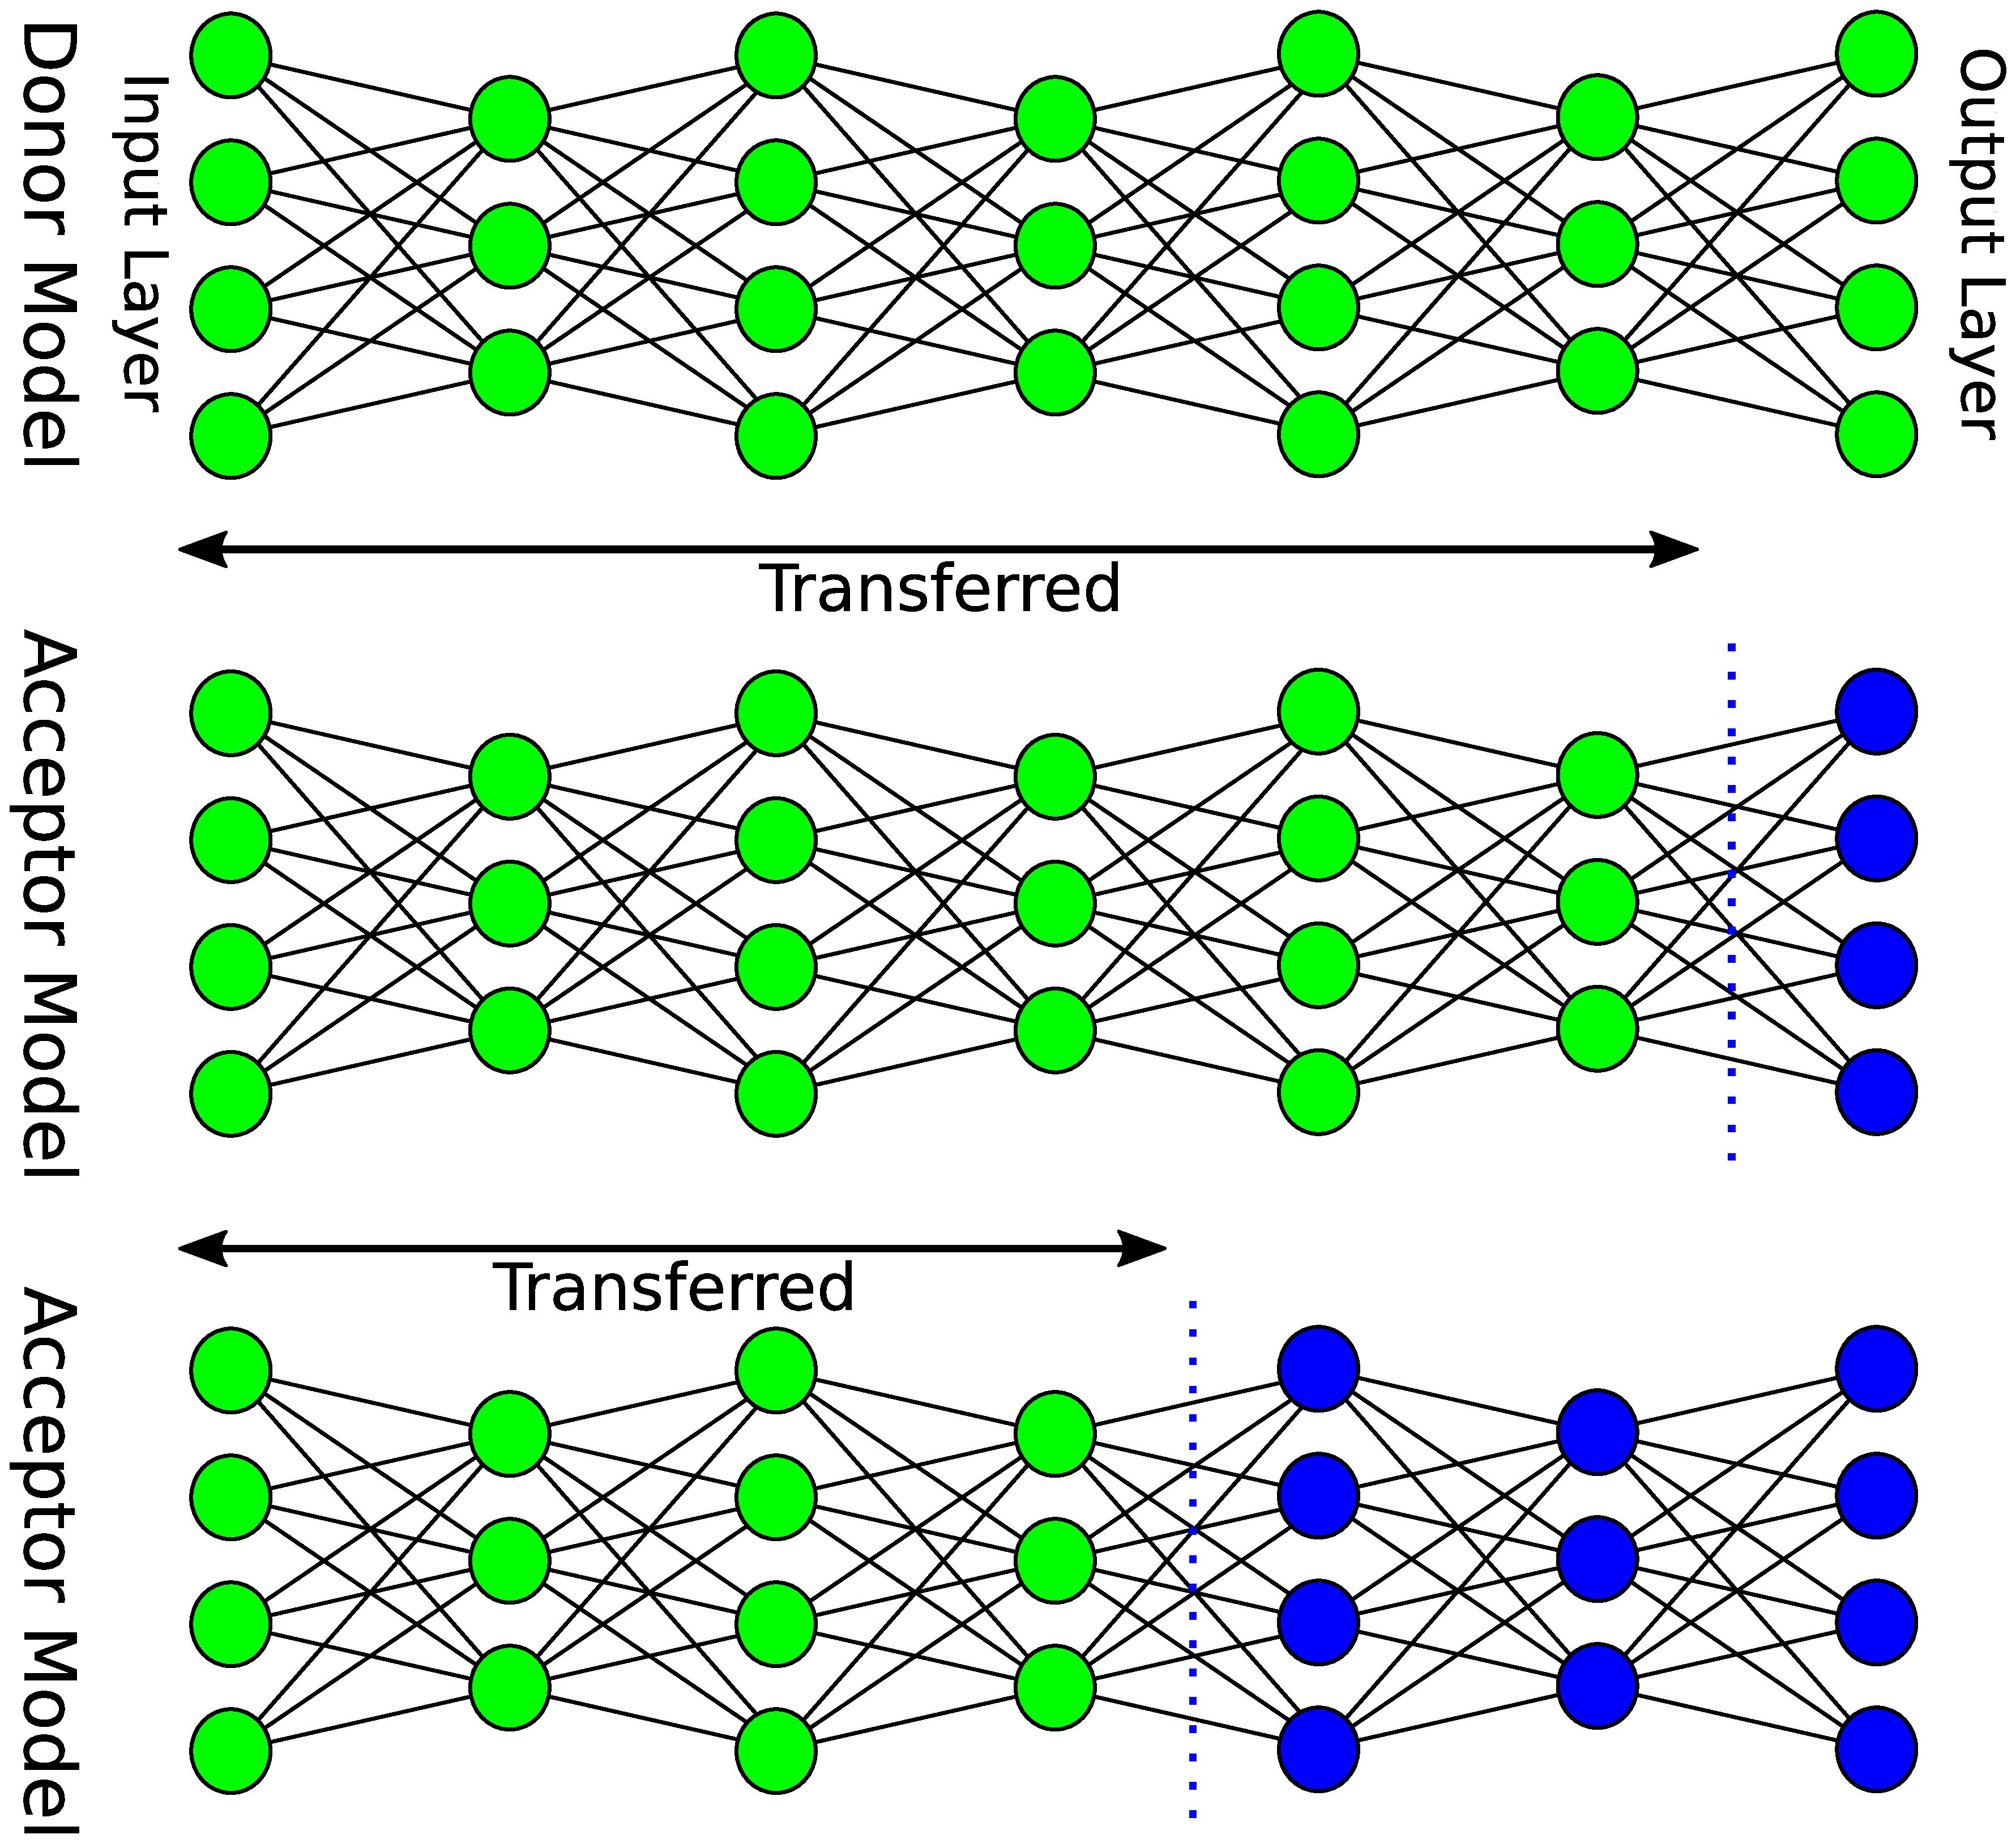
\includegraphics[width=0.7\textwidth]{ann4}
\caption{How weights are transfered from the donor model to the acceptor model in ANN}\label{fig:ann4}
\end{figure}


\begin{figure}[!h]
\centering
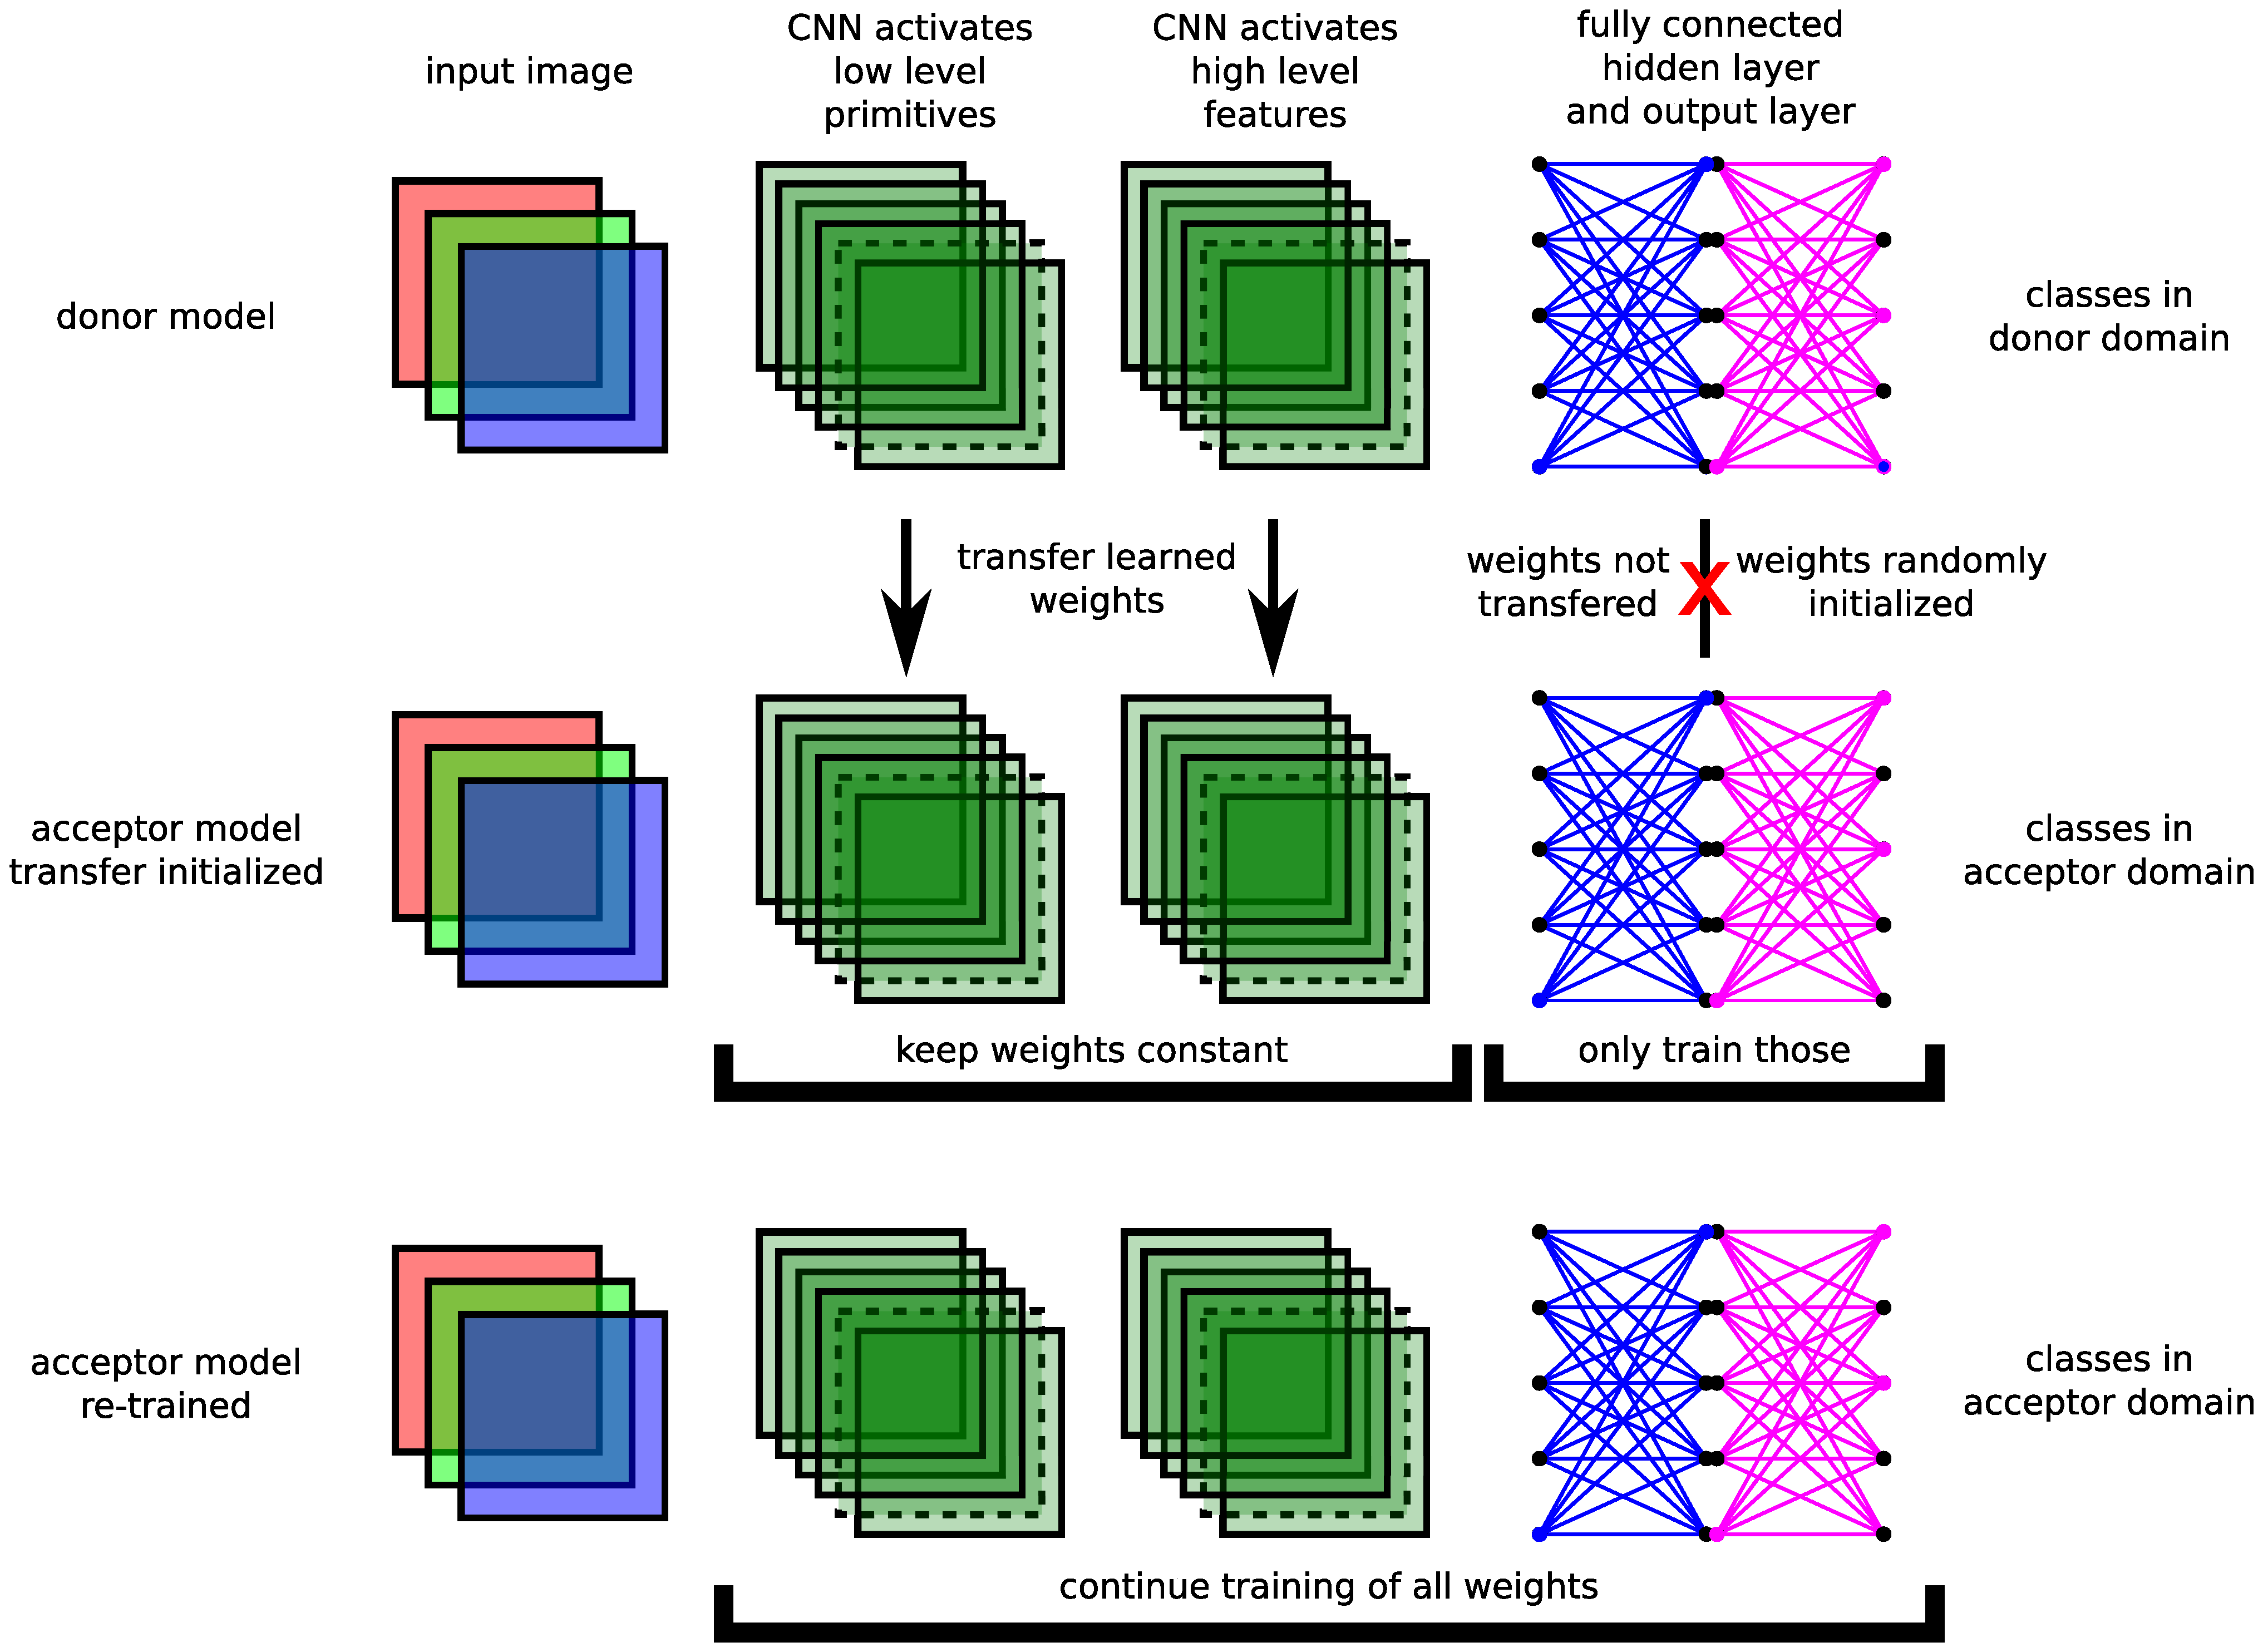
\includegraphics[width=0.7\textwidth]{cnn-doner-acceptor}
\caption{How weights are transfered from the donor model to the acceptor model in CNN}\label{fig:cnn-doner-acceptor}
\end{figure}

\subsection{Estimating performance of fine-tuning off-the-shelf models}


Fine-tuning some models were found to be way more slower than others,
to identify the factors that affects the speed of training and fine-tuning,
two networks that have very different properties were studied:
VGG-16\autocite{simonyan2014very} which has 15 billion multiplication-accumulation operations and around 140 million weights
75\% of which are in a single bottleneck layer (that is FC6), 
and GoogLeNet or Inception v1\autocite{szegedy2015going} which have small fraction of that, that is
less than 1.5 billion multiplication-accumulation operations and less than ten million weights
and the weights are almost evenly distributed on layers.

The number of weights left for training varies from model to another,
so do number of multiplication-accumulation operations, for example,
assuming you have \(n\) classes, in VGG-16\autocite{simonyan2014very},
the fully connected layers are FC6, FC7, and FC8,
one can just retrain FC8 (which has \(4096\times n\) weights)
or the whole fully connected ANN starting from FC6 (which is 120 million more weights than FC8 only).
or the whole CNN network having 138 million weights,
for more details refer to table \ref{table:vgg}.

All experiments in this section were done with 8 images per batch per step, and measure the time needed to reach 500 steps.
Table \ref{table:fine-tune-vgg16} shows the time and accuracy of different fine-tuning settings
of VGG16\autocite{simonyan2014very} on toy dataset of \href{http://download.tensorflow.org/example_images/flower_photos.tgz}{five flowers}

VGG16\autocite{simonyan2014very} pre-trained on ImageNet's ILSVRC 2012\autocite{deng2012imagenet}
which was previously analyzed in table \ref{table:vgg}.
The number of multiplication/addition operations is about 15,470M operation
to be exact it's \(15466168320+4096\times n\) where \(n\) is number of classes.
The number of weights to be trained is last layer (named ``FC8'') is \( 4096\times n \),
while number of weights in previous layers does not depend on number of classes.
As you can see in that table most weights (74.3\%) are in ``FC6'' layer.

Formula \ref{eq:t1} estimates training time by assuming it's proportional to number of multiplication/addition operations \(M\)
in forward pass and number of trainable weights \(W\)
and number of multiplication/addition operations in training part \(T\)
which is the same as the number of trainable weights times output width and height (which is usually \(1\times 1\).
Needless to say that those constants depends on the speed of the machine, how it's configured,
how it handles parallelism, and the model design itself (like non-weights operations like pooling, pre-processing, ..etc.).

\begin{equation}
t = C_0 + C_1 \cdot M + C_2 \cdot W + C_3 \cdot T
\label{eq:t1}
\end{equation}

To find \(C_0\) (which is the time to load the model and store it without training),
just run zero steps, and that was 8 seconds.
To find \(C_1\), \(C_2\), and \(C_3\), by substituting last 3 rows from table \ref{table:fine-tune-vgg16}
we get the following linear equation.

\begin{equation}
\begin{bmatrix}
15,466,188,800 &  16,797,696 &  16,797,696 \\
15,466,188,800 & 119,558,144 & 119,558,144 \\
15,466,188,800 & 121,917,440 & 581,980,160
\end{bmatrix}
\times x = 
\begin{bmatrix}
  772.9-8 \\
2,012.242-8 \\
2,016.7-8
\end{bmatrix}
\label{eq:t_vgg}
\end{equation}

we get 

\[ C_1 = 3.64 \times 10^{-8} \]
\[ C_2 = 1.21 \times 10^{-5} \]
\[ C_3 = -5.21 \times 10^{-8} \]

Having negative value for \( C_3 \) indicate that assumption should be changed by removing the term \(C_3 \cdot T\)
removing the effect of number of trainable weights as in formula \ref{eq:t2}

\begin{equation}
t = C_0 + C_1 \cdot M + C_2 \cdot W
\label{eq:t2}
\end{equation}

By substituting first and last rows, and solve the linear equation \ref{eq:t_vgg2}

\begin{equation}
\begin{bmatrix}
15,466,188,800 &      20,480 \\
15,466,188,800 & 121,917,440 
\end{bmatrix}
\times x = 
\begin{bmatrix}
 582.8-8 \\
2016.7-8
\end{bmatrix}
\label{eq:t_vgg2}
\end{equation}

We get

\[C_1=3.71\times 10^{-8} \]
\[C_2=1.18\times 10^{-5} = 316.8 \times C_1 \]

Writing \(C_2\) and \(C_3\) in terms of \(C_1\), we got \ref{eq:t3}

\begin{equation}
t = 8 + C_1 \cdot M + 316.8  C_1 \cdot W
\label{eq:t3}
\end{equation}

Using \ref{eq:t3} substituting second and third rows of table \ref{table:fine-tune-vgg16} 

\[ t_{fc7} = 8 + C_1 \times 15,466,188,800 + C_2 \times  16,797,696 =   780.1 \]
\[ t_{fc6} = 8 + C_1 \times 15,466,188,800 + C_2 \times 119,558,144 = 1,988.9 \]

which is very close from actual value of 772.9 and 2,012.2 with error 0.9\% and 1.1\% respectively.

Repeating same experiment with different dataset, this time with Birds 200\autocite{WahCUB_200_2011},
results are shown in table \ref{table:fine-tune-vgg16-birds200}. Using formula \ref{eq:t1} gave very close values

\[ C_1 = 3.62\times 10^{-8} \]
\[ C_2 = 1.23\times 10^{-5} \]
\[ C_3 = -5.44\times 10^{-8} \]

And when omitting \(T\) term as in formula \ref{eq:t2}, we got the following result

\[ C_1 = 3.69\times 10^{-8} \]
\[ C_2 = 1.20\times 10 ^{-5} = 324.4 C_1 \]
\[ t = 8 + C_1 \cdot M + 324.4  C_1 \cdot W \]

which is very close from our previous result.

Although the cost of trainable weights is 353 times that of multiplications,
in case of fine-tuning last layer as in FC8 layer,
number of multiplication-accumulation operations \(M\)
is 755 thousand times greater than number of trainable weights \(W\).

This huge gap between number multiplication-accumulation operations 
and number weights in case of fine-tuning neglect any effect of number of classes on time
The cost is merely controlled by number of multiplication-accumulation operations in forward pass is almost constant 15,466M
as seen in table \ref{table:fine-tune-vgg16-2}.
Same conclusion applies to Inception v1 as seen in table \ref{table:fine-tune-inception-v1}
where the number of classes does not have any effect of time with fixed trainable layers.

Several experiments were applied on fine-tuning different layers of Inception V1
and results were recorded on table \ref{table:fine-tune-inception-v1}.
Forming an equation similar to \ref{eq:t2} by substituting the time of fine-tuning a single layer of Inception V1
on flowers 5 dataset and that of fine-tuning both last layer and last inception block ``Mixed\_5c''

\begin{equation}
\begin{bmatrix}
1,497,357,312 &     5,120 \\
1,497,357,312 & 1,349,632 \\
\end{bmatrix}
\times x = 
\begin{bmatrix}
 94.0-8 \\
102.8-8
\end{bmatrix}
\label{eq:t_inception_v1_1}
\end{equation}

Solving it would result in:

\[ C1 = 5.74\times 10^{-8} \]
\[ t = 8 + C_1 \cdot M + 114.0  C_1 \cdot W \]

and by applying it on fine-tuning last layer and last two inception blocks ``Mixed\_5c'' and ``Mixed\_5b''

\[ t = 8 + C_1 \cdot M + 114.0  C_1 \cdot W \]
\[ t = 8 + 1,497,357,312 c1 + 2,326,528 c2 = 109.2 \]

which matches the actual observed value of \( 109.5 \) seconds with error of \(0.3\) seconds.

When more classes are included, converging becomes slower as it's harder to reach good accuracy
this is seen in tables \ref{table:fine-tune-vgg16-2} and \ref{table:fine-tune-inception-v1}.

The time needed to fine-tune last layer of Inception V1 is \(3.7\times\)
faster than full training (as in table \ref{table:fine-tune-inception-v1})
and with VGG-16 it's \(5.6\times\) faster (as in table \ref{table:fine-tune-vgg16}).

Not only it's faster but also better accuracy, because:

\begin{itemize}
\item it can run more training steps in same amount of time.
\item all convolution filters/pre-processors and high-level feature-extractors are already trained.
\end{itemize}

This is only valid up to a limit, because the second point does not hold,
the target task might require different pre-processing or feature extractor than source task
to achieve the desired accuracy, in that case fine-tuning can be used for initialization.

\begin{table*}\caption{Comparing fine-tuning VGG-16 performance up to different layers on same Flowers-5 dataset}\label{table:fine-tune-vgg16}
\centering
\begin{small}
\begin{tabularx}{\textwidth}{llrrrrrr}
\toprule
Model & Layer & Classes & \makecell{Total \\ Mults} & \makecell{Trainable \\ Weights} & \makecell{Training \\ Mults} & Time & Accuracy \\
\midrule
VGG-16 & FC8     & 5 & 15,466M &      20K &         20K &   582.8s & 80.0\% \\
VGG-16 & FC7     & 5 & 15,466M &  16,798K &     16,798K &   772.9s & 76.1\% \\
VGG-16 & FC6     & 5 & 15,466M & 119,558K &    119,558K & 2,012.2s & 45.9\% \\
VGG-16 & Conv5-3 & 5 & 15,466M & 121,917K &    581,980K & 2,016.7s & 57.6\% \\
\midrule
VGG-16 & All     & 5 & 15,466M & 134,269K & 15,466,189K & 3,249.8s & 42.7\% \\
\bottomrule
\end{tabularx}
\end{small}
\end{table*}

\begin{table*}\caption{Comparing fine-tuning VGG-16 performance up to different layers on Birds-200 datasets\autocite{WahCUB_200_2011} }\label{table:fine-tune-vgg16-birds200}
\centering
\begin{small}
\begin{tabularx}{\textwidth}{llrrrrrr}
\toprule
Model & Layer & Classes & \makecell{Total \\ Mults} & \makecell{Trainable \\ Weights} & \makecell{Training \\ Mults} & Time & Accuracy \\
\midrule
VGG-16 & FC8     & 200 & 15,467M &     819K &     819K &   588.6s & 22.8\% \\
VGG-16 & FC7     & 200 & 15,467M &  17,596K &  17,596K &   784.1s & 10.0\% \\
VGG-16 & FC6     & 200 & 15,467M & 120,357K & 120,357K & 2,043.9s & 00.5\% \\
VGG-16 & Conv5-3 & 200 & 15,467M & 122,716K & 582,779K & 2,047.8s & 00.3\% \\
\bottomrule
\end{tabularx}
\end{small}
\end{table*}

\begin{table*}\caption{Comparing fine-tuning same layer of VGG-16 network on different datasets}\label{table:fine-tune-vgg16-2}
\centering
\begin{small}
\begin{tabularx}{\textwidth}{llrrrrrr}
\toprule
Model & Layer & Dataset & \makecell{Total \\ Mults} & \makecell{Trainable \\ Weights} & \makecell{Training \\ Mults} & Time & Accuracy \\
\midrule
VGG-16 & FC8  & Cats Dogs 2   & 15,466,176,512 &   8,192 &   8,192 &   582.4s & 99.3\% \\
VGG-16 & FC8  & Flowers 5     & 15,466,188,800 &  20,480 &  20,480 &   582.8s & 80.0\% \\
VGG-16 & FC8  & Pets 37       & 15,466,319,872 & 151,552 & 151,552 &   582.6s & 82.9\% \\
VGG-16 & FC8  & Flowers 102   & 15,466,586,112 & 417,792 & 417,792 &   584.0s & 57.8\% \\
VGG-16 & FC8  & Birds 200     & 15,466,987,520 & 819,200 & 819,200 &   588.6s & 22.8\% \\
\bottomrule
\end{tabularx}
\end{small}
\end{table*}

\begin{table*}\caption{Comparing fine-tuning Inception V1 performance up to different layers on different datasets}\label{table:fine-tune-inception-v1}
\centering
\begin{small}
\begin{tabularx}{\textwidth}{llrrrrrr}
\toprule
Model & Layer & Dataset & Total Mults & \makecell{Trainable \\ Weights} & Time & Accuracy \\
\midrule
Inception V1 & Logits   & Cats Dogs 2   & 1,497,354,240 &     2,048 &   94.0s & 99.3\% \\
Inception V1 & Logits   & Flowers 5     & 1,497,357,312 &     5,120 &   94.1s & 71.8\% \\
Inception V1 & Logits   & Pets 37       & 1,497,390,080 &    37,888 &   94.3s & 75.0\% \\
Inception V1 & Logits   & Flowers 102   & 1,497,456,640 &   104,448 &   94.1s & 18.8\% \\
Inception V1 & Logits   & Birds 200     & 1,497,556,992 &   204,800 &   94.6s & 2.2\% \\
\midrule
Inception V1 & Mixed\_5c & Flowers 5     &  1,497,357,312 & 1,349,632 & 102.8s & 75.0\% \\
Inception V1 & Mixed\_5c & Birds 200     &  1,497,556,992 & 1,549,312 & 103.5s & 8.0\% \\
\midrule
Inception V1 & Mixed\_5b & Flowers 5     &  1,497,357,312 & 2,326,528 & 109.5s & 79.2\% \\
Inception V1 & Mixed\_5b & Birds 200     &  1,497,556,992 & 2,526,208 & 110.8s & 7.0\% \\
\midrule
Inception V1 & All      & Flowers 5     &  1,497,357,312 & 8,718,784 &  355.4s & 61.4\% \\
Inception V1 & All      & Birds 200     &  1,497,556,992 & 9,118,144 &  355.6s & 6.3\% \\
\bottomrule
\end{tabularx}
\end{small}
\end{table*}

\subsection{Effectiveness of smaller batch sizes}

Trying to achieve high accuracy fine-tuning ``The Caltech-UCSD Birds-200-2011 Dataset''\autocite{WahCUB_200_2011}.
The test was done 4 times using 200, 100, 50, and 10 batch size having fixed learning rate of 0.01 and the result
was as in figure \ref{fig:by-step}

Metrics measured on the batch while training (like cross-entropy-loss)
will be over estimated as they will give results based on the small non-representative batch (for example, the ten images in the batch). 
That's why 10\% of dataset were used for validation (more than one thousand image, independent of training batch size) to evaluate the model periodically.

\begin{figure}[!h]
\centering
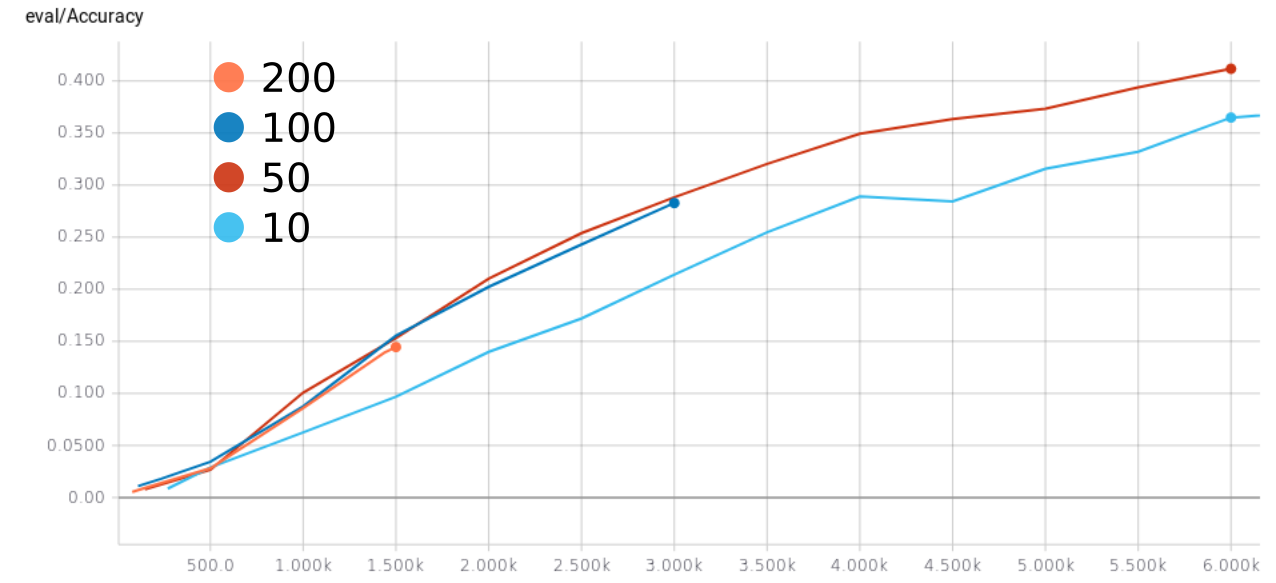
\includegraphics[width=0.7\textwidth]{by-step}
\caption{Top-1 Accuracy fine-tuning Birds 200 dataset with different batch sizes, x-axis is in steps}\label{fig:by-step}
\end{figure}

By looking at accuracy over steps one might think that a batch size of 10 is the worst,
after 1500 step it was only 10\% accuracy, while others were around 15\%.
But this is not a good measure as a batch size of 10 is 5 times faster than batch size of 50,
and 20 times faster than batch size of 200.
By making x-axis measure in time (hours) instead of steps, the result was as in figure \ref{fig:by-time}


\begin{figure}[!h]
\centering
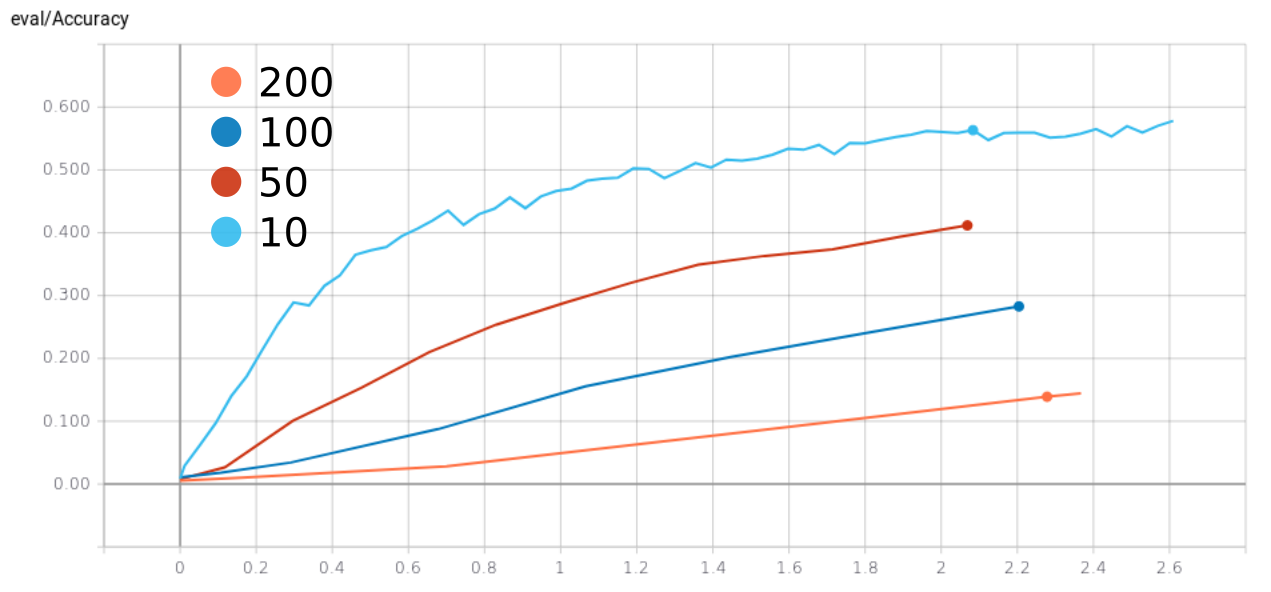
\includegraphics[width=0.7\textwidth]{by-time}
\caption{Top-1 Accuracy fine-tuning Birds 200 dataset with different batch sizes, x-axis is in hours}\label{fig:by-time}
\end{figure}

This is good accomplishment as more than 50\% accuracy was reached in less one and half hour,
specially that this dataset contains too many classes (200) and they look very similar even to expert human.

\subsection{Adaptive batch size}

Previous section showed how small batch size can be effective (as seen in figure \ref{fig:by-time}),
it can make speed of training multiple times faster.
But it will get stuck after some iterations,
that's why one need to use an adaptive approach, that is keep using ``fast-forward'' mode of small batch sizes
as long as it's giving better accuracy compared to previous run,
if not switch to slower mode with larger batch size.


\begin{program}
\begin{verbatim}
1  LET old_accuracy = 0
2  LET batch_size, steps_count = batch_size_normal, steps_count_normal
3  train_steps(steps_count, batch_size)
4  accuracy = evaluate()
5  IF (accuracy>old_accuracy) THEN
6    batch_size, steps_count = batch_size_ff, steps_count_ff
7  ELSE
8    batch_size, steps_count = batch_size_normal, steps_count_normal
9  END IF
10 old_accuracy = accuracy
11 IF not done THEN goto 3
\end{verbatim}
\caption{adaptive batch size algorithm in pseudo code}
\end{program}

More generic algorithm, that is to define some fast forward criteria ``FF\_CRITERIA'',
when satisfied, training settings are set to faster mode in terms of batch size, steps count, learning rate, ..etc.
and when not, normal slower settings are used. 

\begin{program}
\begin{verbatim}
1  init_settings()
2  train_steps()
3  accuracy = evaluate()
4  IF (FF_CRITERIA) THEN
5    apply_settings(ff_settings)
6  ELSE
7    apply_settings(normal_settings)
8  END IF
10 IF not done THEN goto 2
\end{verbatim}
\caption{more general adaptive batch size algorithm in pseudo code}
\end{program}

\subsection{Fine Tuning ``Cat, Dog, or Bird'' with adaptive batch size}

Fine tuning just the last layer of Inception V1 pre-trained on ImageNet 1K classes, is very effective.
The three-classes ``Cat, Dog, or Bird'' database as seen in figure \ref{fig:fine-cats}
took only two hours (on CPU-only setup) to reach 98.9\% top-1 accuracy,
see table \ref{table:cat-dog-bird-metrics} for all metrics, and see confusion matrix in table \ref{table:confusion-cat-dog-bird}.


This is very impressive as this layer only have 3072 trainable weights.

\begin{figure}[!h]
\centering
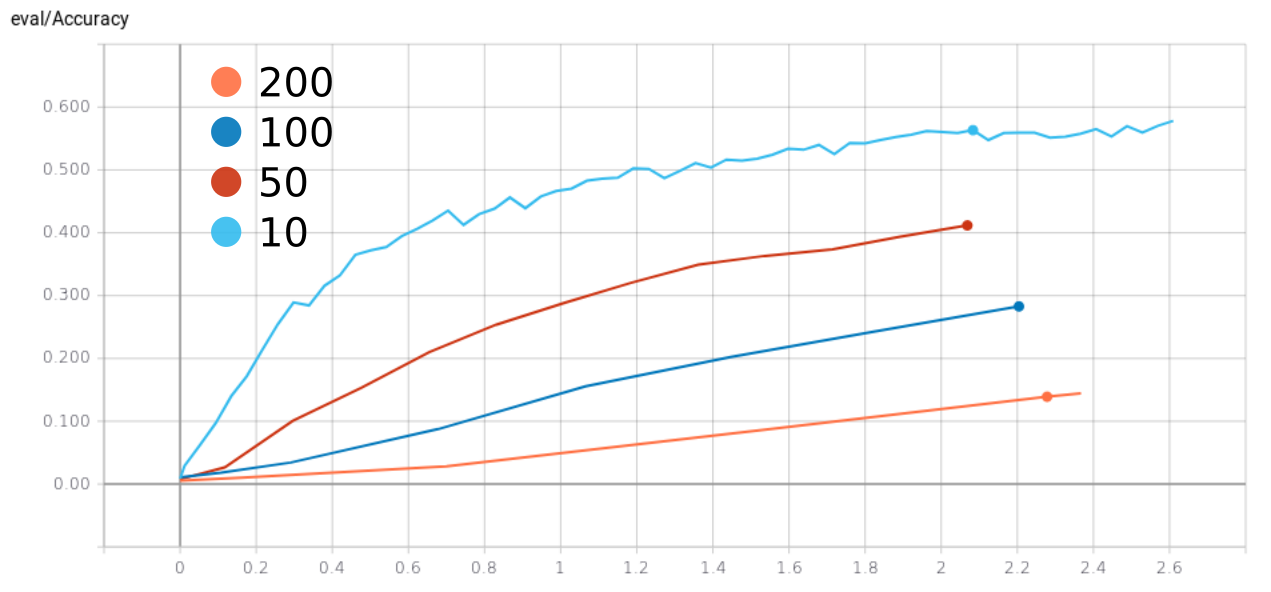
\includegraphics[width=0.7\textwidth]{by-time}
\caption{Accuracy over time (in hours) of fine-tuning last layer of Inception V1 on ``Cat, Dog or Bird'' dataset}\label{fig:fine-cats}
\end{figure}

\begin{table*}\caption{Performance metrics of fine-tuning single layer of Inception v1 on ``Cat, Dog or Bird'' Task}\label{table:cat-dog-bird-metrics}
\centering
\begin{tabularx}{\textwidth}{Xrrrrr}
\toprule
Metric         & Top 1   & Top 2 & Precision & Recall & F1-Score \\
\midrule
Cat, Dog or Bird & 98.90\% & 100\% & 98.86\%   & 98.87\% & 98.87\% \\
\bottomrule
\end{tabularx}
\end{table*}


\begin{table*}\caption{Confusion matric for fune-tuning ``Cat, Dog or Bird'' Task}\label{table:confusion-cat-dog-bird}
\centering
\begin{tabular}{rrrrr}
\toprule
-     &   Cat & Bird & Dog & Total \\
\midrule
Cat   &   428 &    0 &   8 &  436 \\
Bird  &     0 &  455 &   0 &  455 \\
Dog   &     6 &    0 & 383 &  389 \\
\midrule
Total &   434 &  455 & 391 & 1280 \\
\bottomrule
\end{tabular}
\end{table*}


\subsection{Fine Tuning Car Sides Dataset} \label{fine-car-sides}

Same procedure was applied to the nine-classes dataset of car sides. 
And as seen in figure \ref{fig:fine-car-sides-acc},
it reached 82\% top-1 accuracy in less than one hour.
This is impressive because this dataset by design has some confusion
as it's difficult to draw a strict line between back view, partly-back partly-side, and side view,
That's why top-3 accuracy of 99\% was reached as seen in table \ref{table:car-sides-metrics}.

\begin{figure}[!htbp]
\centering
    \begin{subfigure}[b]{\textwidth}
        \centering
        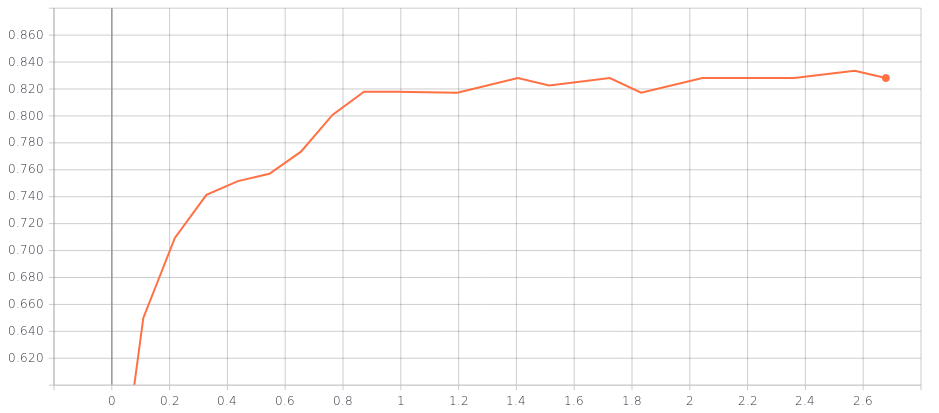
\includegraphics[width=\textwidth]{car-sides-acc}
        \caption{Reaching 82\% top-1 accuracy after in less than one hour of training}
    \end{subfigure}
    \begin{subfigure}[t]{0.48\textwidth}
        \centering
        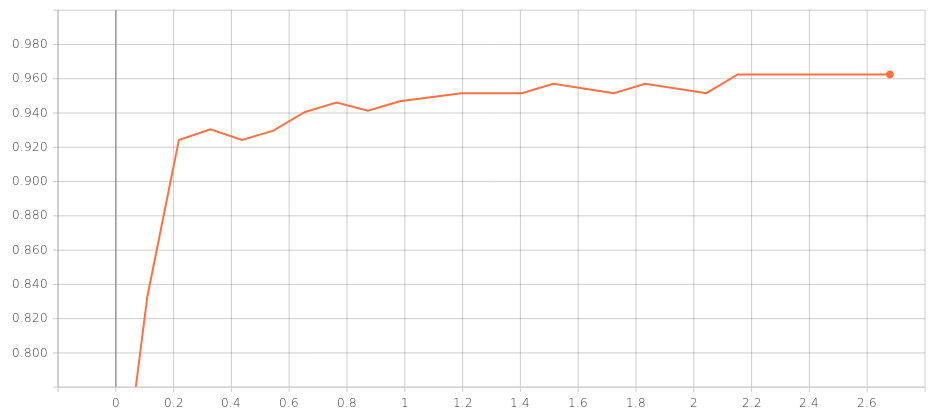
\includegraphics[width=\textwidth]{car-sides-top2}
        \caption{Reaching 96\% top-2 accuracy in about two hours of training}
    \end{subfigure}
    \begin{subfigure}[t]{0.48\textwidth}
        \centering
        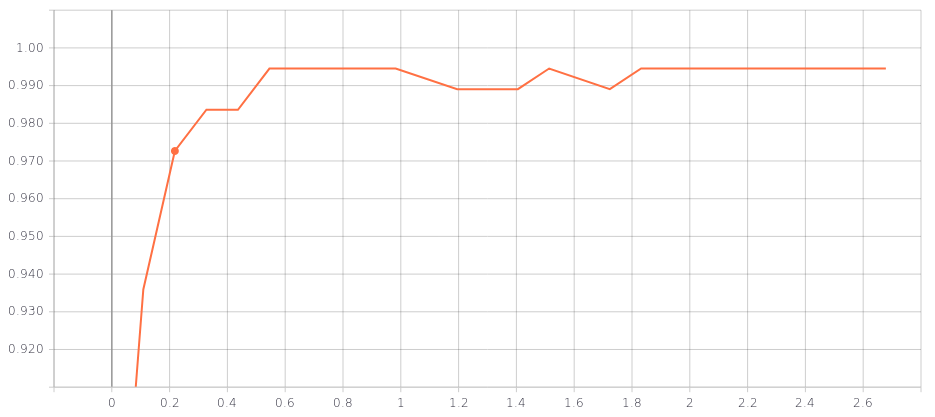
\includegraphics[width=\textwidth]{car-sides-top3}
        \caption{Reaching 99\% top-3 accuracy in about one hour of training}
    \end{subfigure}
\caption{Top-1, Top-2 and Top-3 Accuracy over time (in hours) Fine-Tuning last layer of pre-trained Inception v1 on 9-classes car sides dataset}\label{fig:fine-car-sides-acc}
\end{figure}

\begin{table*}\caption{Performance metrics of fine-tuning single layer of Inception v1 on ``Car sides'' Task}\label{table:car-sides-metrics}
\centering
\begin{tabular}{lrrrrrrr}
\toprule
Metric         & Top 1   & Top 2 & Top 3 & top 5 & Precision & Recall & F1-Score \\
\midrule
Car Sides 9 & 83.36\% & 96.25\% & 99.45\% & 100.00\% & 85.14\% & 79.71\% & 82.34\% \\
\bottomrule
\end{tabular}
\end{table*}


\subsection{Failure of stalling accuracy of fine-tuning of single layer}

ImageNet 1K-classes has so many generic high-level features and it can be easily fine-tuned into identifying a cat from dog.
But if the task is very specific to the level that the already learned generic features are not sufficient to achieve accuracy.
Birds-200-2011 Dataset\autocite{WahCUB_200_2011}, has 200 breads of birds, many of them look very similar even to human eyes
as you can see in figure \ref{fig:confusion-birds200}.
And as seen in figure \ref{fig:fine-birds200-acc}, fine-tuning of a last layer got stuck at around 55\% for more than two and half hours.

\begin{figure}[!htbp]
\centering
    \begin{subfigure}[t]{0.48\textwidth}
        \centering
        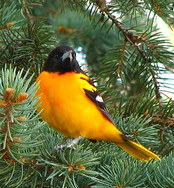
\includegraphics[width=\textwidth]{birds200-baltimore-oriole}
        \caption{An image labeled with ``Baltimore Oriole''}
    \end{subfigure}
    \begin{subfigure}[t]{0.48\textwidth}
        \centering
        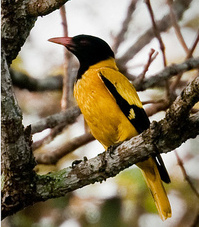
\includegraphics[width=\textwidth]{birds200-hooded-oriole}
        \caption{An image labeled with ``Hooded Oriole''}
    \end{subfigure}
\caption{Two bird breads that look similar even to some humans}\label{fig:confusion-birds200}
\end{figure}


\begin{figure}[!h]
\centering
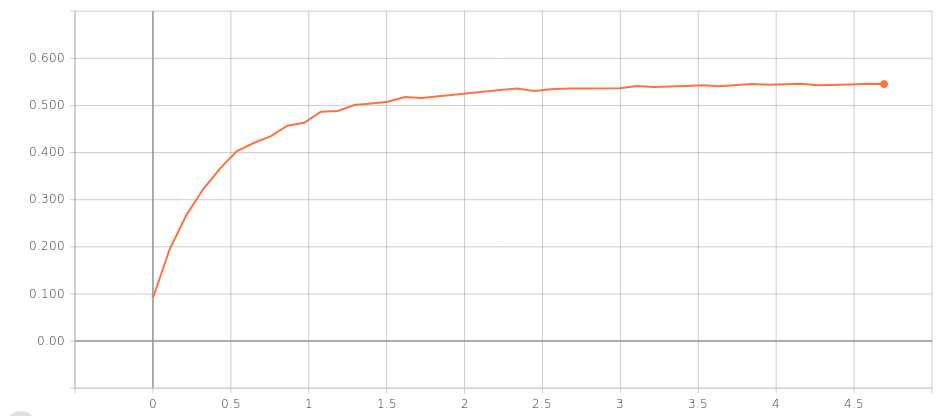
\includegraphics[width=0.7\textwidth]{birds200-acc}
\caption{Accuracy over time (in hours) of fine-tuning last layer of Inception V1 on ``Birds-200'' dataset}\label{fig:fine-birds200-acc}
\end{figure}

The solution to this problem is to either add extra layers that are not part of the original design of the ConvNet,
or include more layers in the training process after fine-tuning a single layer as in figure \ref{fig:ann4}.

Since Inception v1 has branches, the first layer just before last layer (Logits) is an entire inception module block named
``Mixed\_5c'' consisting of four branches similar to that in figure \ref{fig:inception-block} previously discussed in section \ref{sec_inception_v1}.

Figure \ref{fig:fine-birds200-5c} shows that including an inception module block beside last fully connected layer
was able to push accuracy from 55\% to 60\% within one and half hours for more metrics refer to table \ref{table:birds200-metrics}.

\begin{figure}[!h]
\centering
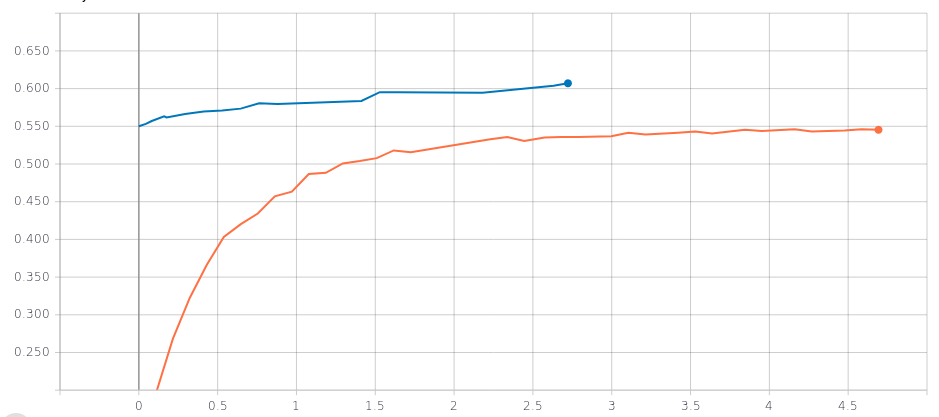
\includegraphics[width=0.7\textwidth]{birds200-5c}
\caption{Accuracy over time (in hours) of fine-tuning a block ``Mixed\_5c'' (blue) along with last layer (orange) of Inception V1 on ``Birds-200'' dataset}\label{fig:fine-birds200-5c}
\end{figure}

\begin{table*}\caption{Performance metrics of fine-tuning single layer of Inception v1 on ``Birds-200'' Task}\label{table:birds200-metrics}
\centering
\begin{small}
\begin{tabularx}{\textwidth}{Xrrrrrrr}
\toprule
Birds 200 & Top 1   & Top 2 & Top 3 & top 5 & Precision & Recall & F1-Score \\
\midrule
Logits    & 54.30\% & 70.23\% & 77.19\% & 84.69\% & 55.56\% & 56.29\% & 55.92\% \\
Mixed-5c  & 60.39\% & 74.14\% & 81.17\% & 88.13\% & 61.81\% & 62.34\% & 62.08\% \\
\bottomrule
\end{tabularx}
\end{small}
\end{table*}


\subsection{The problem of ``none'' class}

When training a model that distinguish a car from a none car,
then the needed dataset should have images for cars and all kind of non-cars.
It's very easy to have a dataset of car front view, car back view, car side view
but adding a fourth class ``none'' is very difficult, because it would require
having photos all kinds of other things (animals, humans, plants, ...etc.).

Trying to add opposite of the mean vector of the classes did not work at all.
Taking weights from ImageNet and averaging none-car vectors resulted on almost zero vector.
Passed weight vectors to ``sign()'' function showed that
each feature has almost equal number of positive and negative items,
which is the reason why averaging did not work, and components canceled each other.

That's why a different way is needed to calculate weights vector of ``none'' class.

\subsection{Jointly Activated Classes and Cosine Similarity}

When a pivot class is taken (like ``wagon''), its weights vector \(\hat{v}_i\)
can be compared to other classes \(\hat{v}_j\) using cosine similarity,
and when using unit vectors, the similarity equals to the dot product as in \ref{eq:cosine_similarity}

\begin{equation}
\cos \theta = \frac{ \vec{v}_{i}\cdot \vec{v}_{j} }{ |\vec{v}_{i}| \cdot |\vec{v}_{j}| } = \hat{v}_{i}\cdot \hat{v}_{j}
\label{eq:cosine_similarity}
\end{equation}

The result would be in the interval [-1, +1] from where -1 means the opposite and 1 means exact match.
Table \ref{table:cosine_classes} shows top similar and dissimilar classes to some chosen pivots.

\begin{definition}{Jointly-Activated Classes:}
Two classes are said to be ``Jointly-Activated Classes'' if the dot product of their weights unit vectors is positive
(they have positive positive cosine similarity).
\label{def:jointly_activated}
\end{definition}

In a diverse and rich CNN like ImageNet models,
the number of similar classes is found to be very close to dissimilar,
that is having ~450 positive similarity and ~550 negative similarity
(as seen in first column of table \ref{table:cosine_classes}).
Which make it possible to use zero as threshold between similar and dissimilar.

For other models one might set a different threshold other than zero.
One might use a percentile-based threshold, the 50th-percentile would take half of the classes as similar,
setting the threshold to the 75th-percentile would take only 25\% of the classes as similar,
and the rest 75\% as dissimilar.


\begin{definition}{Tolerated Jointly Activated Classes:}
For a given tolerance \(\tau\), two classes are said to be ``Tolerated Jointly-Activated Classes''
if the dot product of their weights unit vectors is greater than of equal \(\tau\).
\begin{equation}
\hat{v}_{i}\cdot \hat{v}_{j} \geq \tau
\label{eq:tol_jointly_activated}
\end{equation}
\label{def:tol_jointly_activated}
\end{definition}

% TODO: congruence subgroups

One can't partition classes into ``Equivalence Classes'' directly using jointly activated classes
because they do not form a partition on the set of classes. But there are many ways of partitioning the classes,
one of them is by taking the class having the largest magnitude of weight vector, then find all jointly activated classes
then only take a fixed percentile of the similarity, remove most similar classes then repeat. 

\begin{table*}\caption{Cosine Similarity between ImageNet Classes measured on MobileNet weights. Under pivot classes two numbers are shown, number of similar classes and dissimilar classes}\label{table:cosine_classes}
\centering
\begin{tabularx}{\textwidth}{lXrXr}
\toprule
Pivot Class & Top Similar Classes & \% & Top Dissimilar Classes & \% \\
\midrule
\multirow{5}{*}{\makecell{437:Wagon \\ +443 -557 }} & 657:minivan & 24.7\% & 611:T-shirt & 11.3\% \\
 & 512:convertible & 22.4\% & 778:scabbard & 10.6\% \\
 & 610:jeep & 20.4\% & 595:harp & 10.1\% \\
 & 628:limousine & 19.2\% & 328:starfish & 10.0\% \\
 & 582:radiator grille & 17.4\% & 924:plate & 09.7\% \\
% & 469:cab taxi & 17.1\% & 928:trifle & 09.5\% \\
% & 718:pickup & 14.4\% & 986:daisy & 09.5\% \\
% & 676:moving van & 14.1\% & 126:hermit crab & 09.4\% \\
% & 661:mobile home & 14.0\% & 812:space heater & 08.5\% \\
% & 655:minibus & 13.4\% & 101:black swan & 08.3\% \\
\midrule
\multirow{5}{*}{\makecell{852:television \\ +441 -559}} & 783:CRT screen & 27.4\% & 54:ring-neck snake & 09.0\% \\
 & 599:home theater & 24.6\% & 936:mashed potato & 08.8\% \\
 & 549:entertainment center & 24.1\% & 318:leafhopper & 08.4\% \\
 & 665:monitor & 23.8\% & 484:castle & 07.9\% \\
 & 528:desktop computer & 15.1\% & 162:basset hound & 07.7\% \\
% & 652:microwave & 14.8\% & 650:megalith & 07.7\% \\
% & 476:car mirror & 12.1\% & 25:great gray owl & 07.4\% \\
% & 917:web site & 12.0\% & 994:gyromitra & 07.4\% \\
% & 531:digital clock & 11.6\% & 380:howler monkey & 07.4\% \\
% & 591:hand-held computer & 11.6\% & 995:stinkhorn & 07.4\% \\
\midrule
\multirow{5}{*}{\makecell{285:Siamese cat \\ +443 -557}} & 286:Egyptian cat & 20.6\% & 298:sloth bear & 11.0\% \\
 & 288:lynx & 19.7\% & 818:sports car & 10.9\% \\
 & 255:pug & 19.7\% & 308:weevil & 10.0\% \\
 & 226:malinois & 19.0\% & 545:Dutch oven & 09.9\% \\
 & 287:cougar & 16.9\% & 123:American lobster & 09.8\% \\
% & 389:giant panda & 16.7\% & 32:tree frog & 08.9\% \\
% & 284:Persian cat & 16.6\% & 523:croquet ball & 08.7\% \\
% & 360:black-footed ferret & 14.9\% & 11:brambling & 08.7\% \\
% & 196:Boston bull & 14.6\% & 767:rotisserie & 08.5\% \\
% & 17:bulbul & 13.7\% & 925:guacamole & 08.4\% \\ 
\midrule
\multirow{5}{*}{\makecell{89:macaw \\ +432 -568}} & 91:lorikeet & 34.8\% & 535:dish washer & 11.5\% \\
 & 88:African gray parrot & 26.3\% & 175:Norwegian elkhound & 10.7\% \\
 & 97:toucan & 24.5\% & 71:Phalangium opilio & 09.7\% \\
 & 90:sulphur-crested cockatoo & 24.5\% & 180:Staffordshire bullterrier & 09.2\% \\
 & 93:bee eater & 23.1\% & 55:hognose snake & 09.0\% \\
% & 15:indigo bird & 19.0\% & 759:reel & 08.9\% \\
% & 94:hornbill & 18.9\% & 733:Polaroid Land camera & 08.9\% \\
% & 18:jay & 17.2\% & 161:Afghan hound & 08.7\% \\
% & 96:jacamar & 16.9\% & 351:ibex & 08.6\% \\
% & 85:peacock & 15.5\% & 552:face powder & 08.5\% \\
\bottomrule
\end{tabularx}
\end{table*}

\subsection{Category Adaptation using Fuzzy logic on Cosine similarity}

Given pivot class (or classes or a weight unit vector),
instead of creating ``none'' class by averaging vectors of all other classes
and suffering from weights canceling each other,
one can average only dissimilar classes
(either those negative cosine similarity or with cosign similarity below some percentile-based threshold)
or even better give weights to all other classes by their dissimilarity (\(1-similarity\)).

Depending on the model and how feature space is distributed,
a negative feature might never appear due to ReLU activation from previous layers,
that's why a non-negative multiplier on weights unit vectors is needed
so that the resulting direction of unit vector is valid in feature space.
To find the unit vector of ``none'' class, one can exclude similar unit vectors similar classes
instead of multiply them by negative number.
Event better one might use probabilistic similarity\ref{def:prob_sim} and fuzzy logic.

\begin{definition}{Probabilistic Similarity:}
For a given cosine similarity \(S_{ij}\) between classes \(i\) and \(j\),
the probabilistic similarity \(p^d_{ij}\) is defined to be
\begin{equation}
p^s_{ij} = \frac{1+S_{ij}}{2} = \frac{ 1+\hat{v}_{i}\cdot \hat{v}_{j} }{2}
\label{eq:prob_sim}
\end{equation}
\label{def:prob_sim}
\end{definition}

\begin{definition}{Probabilistic Dissimilarity:}
The probabilistic dissimilarity \(p^d_{ij}\) is defined to be
\begin{equation}
p^d_{ij} = 1 - p^s_{ij}
\label{eq:prob_dissim}
\end{equation}
\label{def:prob_dissim}
\end{definition}

The probabilistic version of similarity\ref{eq:prob_sim} and dissimilarity\ref{eq:norm_dissim} are in the range [0, 1].
And since it's in that range it can also be treated as probability
and apply fuzzy logic-like operations like ``AND''/``OR'' using addition for ``OR'' (as in formula \ref{eq:vec_cat_adapt})
and multiplication for ``AND''.

For example, if one wants ``not this class'' and ``not that class''
one can use multiplication as in \ref{eq:joint_dissim}

\begin{definition}{Joint Probabilistic Dissimilarity:}
Given multiple classes \(c_1,c_2,c_3 \ldots c_n\), the joint probabilistic dissimilarity of them against a given class \(c_j\)
is the multiplication of all normalized dissimilarity
\begin{equation}
\prod_{i} p^d_{ij}
\label{eq:joint_dissim}
\end{equation}
\label{def:joint_dissim}
\end{definition}



\subsection{Injecting ``None'' class using weights manipulations}

As discussed before in equation \ref{eq:ann_weights} the weights matrix is composed of vectors in feature space,
one can use a formula similar to \ref{eq:vec_cat_adapt} create ``none'' class, 
for example, if we have Bird, Cat or Dog model, we can inject a fourth class of ``none of them''.

''Non-car`` class were injected into the CNN that identifies car sides in section \ref{fine-car-sides}
so the result is a model that can identify cars from non-cars,
and if it's a car it would indicate from which side the picture was taken.
As seen in figure \ref{fig:cat-car-side},
a cat picture which was previously identified as front side view is now identified as ``none''


\begin{figure}[!h]
\centering
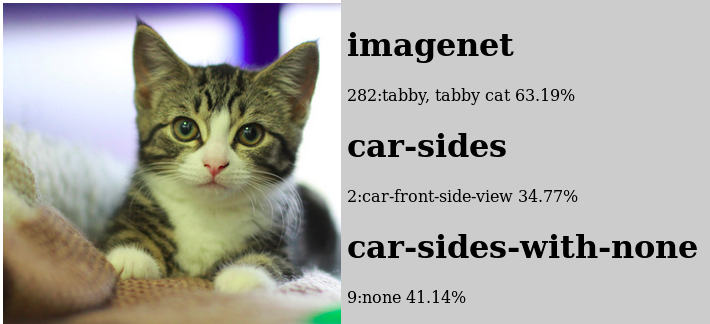
\includegraphics[width=0.7\textwidth]{cat-car-side}
\caption{Cat mistakenly identified as car front side view before model is manipulated to get it identified as ``none''}\label{fig:cat-car-side}
\end{figure}

\subsection{Fine-Tuned CNN to Cleanup Dataset}

Figure \ref{fig:front-side} and \ref{fig:back-side} shows that the design identity of a car
is mainly seen in the front and back view.
It's less likely for a human expert to identify car's make and model from a picture of the interior (seats and dashboard).
There are many cars that looks similar from a perfect side view specially if they both are sedan or SUV.

Inception v1 ImageNet were fine-tuned on ``Vehicle Viewing Angles Dataset'', then 
injected non-cars using weights manipulation as in a previous section, 
The resulted model was used to clean up the noisy dataset,
by removing interior pictures, side pictures, and non-cars.

\begin{figure}[!htbp]
\centering
    \begin{subfigure}[t]{0.48\textwidth}
        \centering
        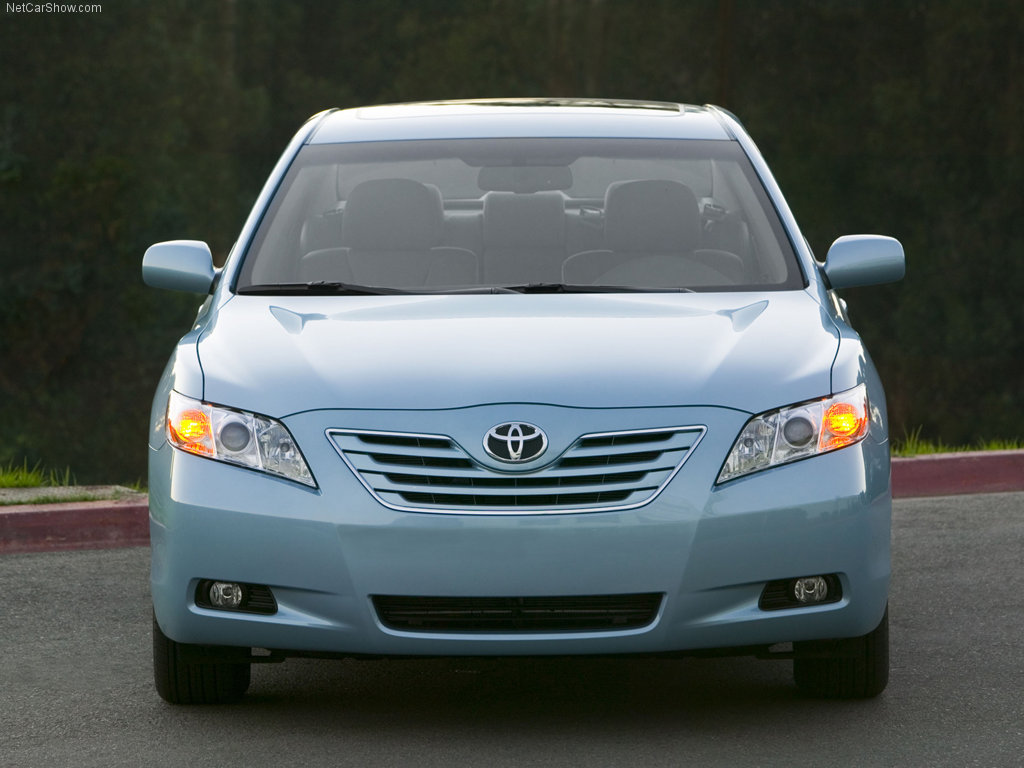
\includegraphics[width=\textwidth]{camry-front}
        \caption{Toyota Camry Front View}
    \end{subfigure}
    \begin{subfigure}[t]{0.48\textwidth}
        \centering
        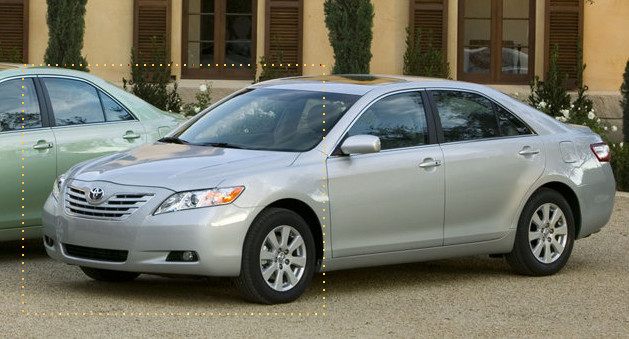
\includegraphics[width=\textwidth]{camry-side-front}
        \caption{Toyota Camry side view with partial front view}
    \end{subfigure}
\caption{How the partly-front partly-side view of this car carries the design identity of front view}\label{fig:front-side}
\end{figure}

\begin{figure}[!htbp]
\centering
    \begin{subfigure}[t]{0.48\textwidth}
        \centering
        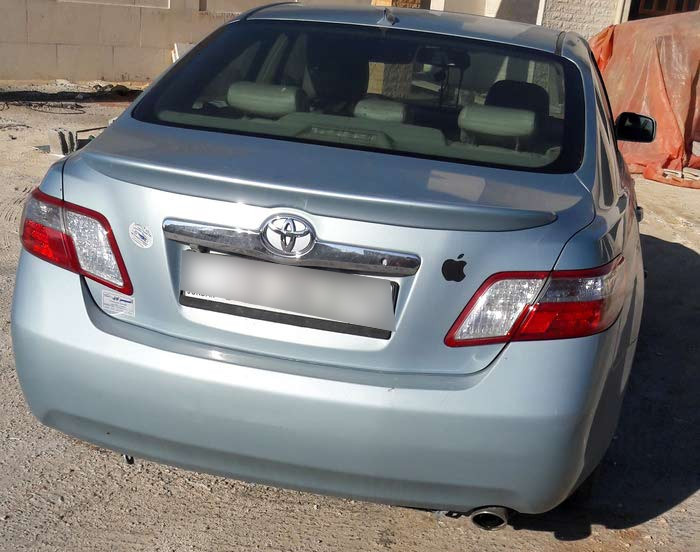
\includegraphics[width=\textwidth]{camry-back}
        \caption{Toyota Camry Back View}
    \end{subfigure}
    \begin{subfigure}[t]{0.48\textwidth}
        \centering
        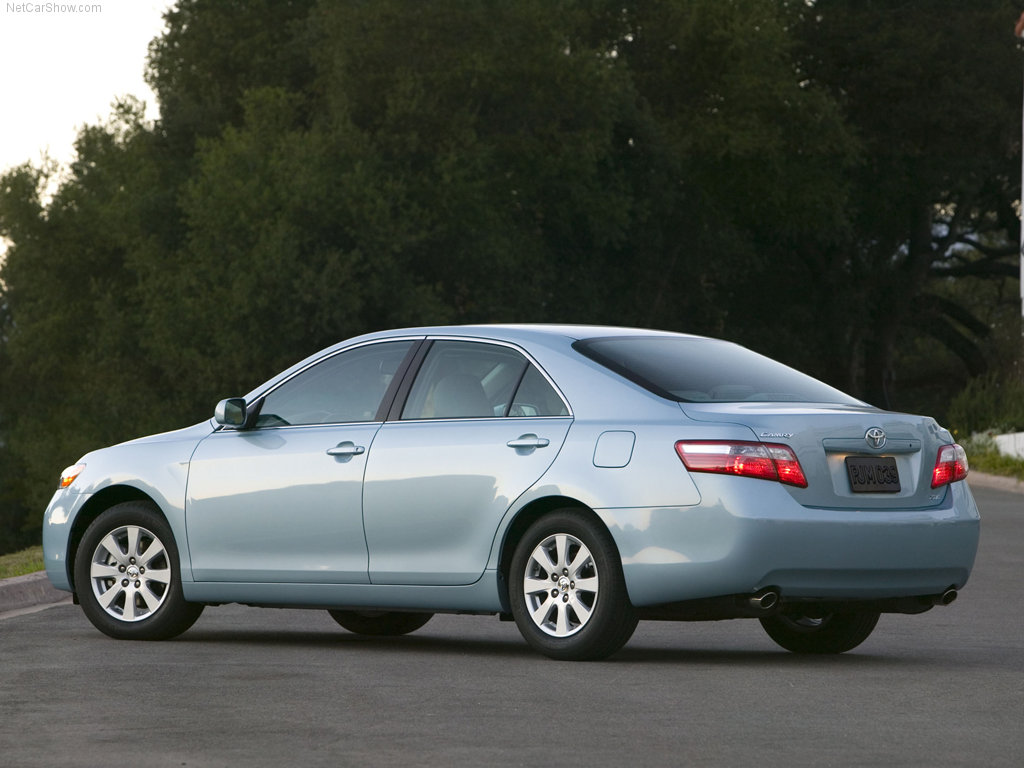
\includegraphics[width=\textwidth]{camry-side-back}
        \caption{Toyota Camry side view with partial back view}
    \end{subfigure}
\caption{How the partly-back partly-side view of this car carries the design identity of back view}\label{fig:back-side}
\end{figure}

\subsection{Fine-tuning small number Make/Models/Years}

The goal of this research is to identify car's make/model/year from its picture.
Initially, toy problem of recognizing very small number of popular sedan make/model/years was examined:

\begin{enumerate}
\item Honda,Civic,1996-2000
\item Honda,Civic,2001-2005
\item Honda,Civic,2006-2008
\item Hyundai,Avante,HD-2007-2010
\item Hyundai,Avante,MD-2011+
\item Hyundai,Avante,Old-1990-1999
\item Hyundai,Avante,XD-2000-2006
\item Toyota,Camry,2007-2011
\item Toyota,Camry,2012-2017
\end{enumerate}

Inception V1 model pre-trained on ImageNet 1K task was fine-tuned on those nine classes task by just training last layer.

\subsection{Fine-tuning 110-classes of Make/Models/Years}

110 make/models/years were included from top sold cars,
that collectively form more than 70\% of cars sold in the region.
Some models are almost identical that get rebadged differently by different dealers in different countries, 
for example, ``Hyundai Elantra'' is rebadged as ``Hyundai Avante'', and ``Chevrolet Tahoe'' which is rebadged ``GMC Yukon''.
For this reason, only one of them is picked in the dataset.
And if two cars looks very similar, we only pick the most popular one.

Accuracy of 80\% top-1 single picture was achieved after two weeks of training. This is very impressive result because,
users upload 5 pictures on average, using the previous side model, front or back views can be given higher priority
which will result on more accurate results.

\subsection{Faster way to including one more car model: ``Introduced Confusion''}

Given a model that can identify 110 make model year, that needs to be extended to include one more car model
Making it 111-classes task without repeating weeks of training.
To add ``Mercedes-Benz G-Class'' to the 110-models task.
Passing a sample of training data to the old 110-classes model which does not have G-Class, 
and identify most frequent class that is confused with it, in that case it was Toyota Land Cruiser 2012.
Weights were crafted in last layer of target task, by taking source task's weights 
of size \(1024\times110\), extending it to size \(1024\times111\)
by duplicating weights corresponding to ``Toyota Land Cruiser 2012''
into those corresponding to the newly added class ``Mercedes-Benz G-Class''
And craft bias values in a similar way. This is merely a good initialization.
This proposed technique is called ``Introduced Confusion''.

The initial Top-1 accuracy dropped from 80\% in source task to 75\% in target task,
but after 6 hours of fine-tuning it recovered and reached 80\%.
But top-1 accuracy is not the metric to look for (as a stop condition),
but it should be confusion matrix as it should recover, if measured before training
all Benz G-class would be wrongly predicted as Toyota Land Cruiser, after enough training
the top confusion should return to what it was before ``Introduced Confusion''.

This procedure can be used multiple times,
This technique was used to extend 110-classes task into 116-classes task
without any notable sacrifice in accuracy metrics as seen in table \ref{table:car-models-metrics}.
And the confusion matrix after training have recovered reporting the same top confusing classes as what was before.


\begin{table*}\caption{Performance metrics of fine-tuning Inception v1 on ``Car-Models'' Task}\label{table:car-models-metrics}
\begin{adjustwidth}{-2in}{-2in} %
\centering
\begin{tabular}{@{}lrrrrrrr@{}}
\toprule
task            &   Top 1 &   Top 2 &   Top 3 &   Top 5 & Precision & Recall & F1-Score \\
\midrule
Car Models 110  & 79.53\% & 87.89\% & 89.92\% & 91.88\% & 78.82\% & 70.47\% & 74.41\% \\
Car Models 116  & 79.22\% & 87.19\% & 89.92\% & 92.34\% & 77.87\% & 72.13\% & 74.89\% \\
Car Models 134  & 76.80\% & 87.19\% & 90.00\% & 92.42\% & 77.10\% & 74.27\% & 75.66\% \\
Car Models 205  & 79.53\% & 89.14\% & 91.95\% & 94.53\% & 79.70\% & 78.42\% & 79.06\% \\
Car Models 229  & 81.17\% & 88.20\% & 90.94\% & 93.67\% & 80.89\% & 79.70\% & 80.29\% \\
\bottomrule
\end{tabular}
\end{adjustwidth}
\end{table*}


\subsection{Oversampling The Crafted Confusion}

The previous method extended the trained model saving weeks of training time to include one more class.
By crafting weights creating confusion between the newly added class (Benz G-Class) and one of the existing classes (Toyota LC).
Since stochastic training is used with adaptive mini-batches (mostly of 8 images) and
assuming equally likely distribution of classes,
then the probability of having a batch that has both ``Toyota Land Cruiser 2012'' and ``Mercedes-Benz G-Class''
is less than 0.5\% which means after 1000 steps,
it would have seen less than 5 batches that can train it on how to resolve this confusion.

To overcome this limitation, we need to over-sample images that belong to the newly injected class
and the one that it was used to initialize it creating confusion,
in our case to over-sample ``Toyota Land Cruiser 2012'' and ``Mercedes-Benz G-Class''
and to under-sample the rest classes.

This should be done for limited number of steps, just to recover the created confusion,
then continue using normal fair sampling.
The criteria can be based on number of steps or based on accuracy or confusion matrix.

% The Oxford-IIIT Pet Dataset\autocite{parkhi12a}
% inception v1
% real    7m4.682s
% 2018-01-05 21:00:03.394634: I tensorflow/core/kernels/logging_ops.cc:79] eval/Recall_5[0.12]                                                          
% 2018-01-05 21:00:03.394644: I tensorflow/core/kernels/logging_ops.cc:79] eval/Accuracy[0.02125]    

% nasnet mobile
% real    11m14.126s 
% 2018-01-05 21:36:54.890997: I tensorflow/core/kernels/logging_ops.cc:79] eval/Accuracy[0.0175]                                                        
% 2018-01-05 21:36:54.890997: I tensorflow/core/kernels/logging_ops.cc:79] eval/Recall_5[0.145] 

% mobilenet 500
% real    5m49.873s                    
% 2018-01-05 22:33:00.807913: I tensorflow/core/kernels/logging_ops.cc:79] eval/Accuracy[0.03625]                                                       
% 2018-01-05 22:33:00.807913: I tensorflow/core/kernels/logging_ops.cc:79] eval/Recall_5[0.1575]  

% mobilenet 1500 96batch size
% real    39m18.147s
% 2018-01-05 23:17:58.520072: I tensorflow/core/kernels/logging_ops.cc:79] eval/Recall_5[0.16]                                                          
% 2018-01-05 23:17:58.520087: I tensorflow/core/kernels/logging_ops.cc:79] eval/Accuracy[0.0325]     

% --------------


% find opensooq_photos/ -type f | while read a; do convert $a -resize 300x300'>' "2${a/.png/.jpg}" ; done

% pets37 inception_v1 500 batch=32
% real    27m21.214s                   
% 2018-01-06 17:25:54.824721: I tensorflow/core/kernels/logging_ops.cc:79] eval/Accuracy[0.03125]                                                       
% 2018-01-06 17:25:54.824820: I tensorflow/core/kernels/logging_ops.cc:79] eval/Recall_5[0.1125]  


% cats_dogs nasnet mobile 500 batch=32
% real    48m17.710s                   
% 2018-01-06 16:16:48.384419: I tensorflow/core/kernels/logging_ops.cc:79] eval/Accuracy[0.67375]                                                       
% 2018-01-06 16:16:48.384505: I tensorflow/core/kernels/logging_ops.cc:79] eval/Recall_5[1]    

% inception v1 500 batch=32
% real    27m11.181s                                                                      
% 2018-01-06 16:51:19.159921: I tensorflow/core/kernels/logging_ops.cc:79] eval/Accuracy[0.70125]
% 2018-01-06 16:51:19.159998: I tensorflow/core/kernels/logging_ops.cc:79] eval/Recall_5[1]



% fine tuning 5 flowers dataset, 500 steps using nasnet mobile took user 72m56.263s
% eval took 1m47.632s and eval/Recall_5[1],  eval/Accuracy[0.455]
% real    11m9.539s user    74m47.891s -- eval/Recall_5[1] eval/Accuracy[0.4325] real    0m29.906s user    1m51.915s


% eval took user    1m47.774s eval/Recall_5[1], eval/Accuracy[0.3725]

% inception v2 took 51m44.738s
% eval took 1m12.244s and gave eval/Accuracy[0.7] eval/Recall_5[1]
% ------------

% vgg_16, training real    46m30.582s - user    300m14.216s
% eval eval/Recall_5[1], eval/Accuracy[0.8375]
% eval took real    1m1.862s / user    6m19.953s

% ---------

% vgg_16 fc7, training real    62m44.735s user    346m54.476s

% eval/Accuracy[0.8175] eval/Recall_5[1]
% eval took real    1m2.677s / user    6m20.847s   


% ----------------
% vgg_16 fc6 training real    175m23.351s user    672m57.927s

% eval/Accuracy[0.7525] eval/Recall_5[1] in eval real    1m7.324s user    6m20.416s

% inception v1 pets37
% real    849m53.432s
% 2018-01-08 10:53:45.546915: I tensorflow/core/kernels/logging_ops.cc:79] eval/Recall_5[0.165]                                                         
% 2018-01-08 10:53:45.546915: I tensorflow/core/kernels/logging_ops.cc:79] eval/Accuracy[0.03875]     


% using the already trained network
% as feature extractor or as a pre
% The researcher have found that some more recent 


% 1000x64 Acc=21.3\%, recall_5=52.2\%
% 1000x8



\chapter{Discussion and Recommendations}

\section{Results}

Given Inception V1 model trained to solve ImageNet one thousand classes task which have accuracy of 69.8\% in that task.
Transferring knowledge from that task to solve the task of identifying 229 car models,
high accuracy was achieved as seen in table \ref{table:final-car-models-metrics}.

Top 1 accuracy of 81.17\% with very close Precision and Recall values indicates
that it does not suffer from either false positive problem nor false negative problem.
Compared to the accuracy of original source model (69.8\%)
and the complexity of the target task this is an impressive result.

Another important aspect of this work, that it's expandable, starting with only 110 car models,
then expanded it to 116, 134, 205 and finally to 229 car models.
Each expansion process took only hours.

\begin{table*}[!htbp]\caption{Final model performance for ``Car-Models-229'' Task}\label{table:final-car-models-metrics}
\centering
\begin{tabular}{lr}
\toprule
Metric            &  Value \\
\midrule
Top 1 & 81.17\% \\
Top 2 & 88.20\% \\
Top 3 & 90.94\% \\
Top 5 & 93.67\% \\
Precision & 80.89\% \\ 
Recall & 79.70\% \\
F1-Score & 80.29\% \\
\bottomrule
\end{tabular}
\end{table*}

\section{Model Choice}

There are so many pre-trained models to choose from. Model of choice in this research is Inception v1\autocite{szegedy2015going}
due to its relatively small number of multiplication-accumulation operations
that falls in the same level of MobileNet, but it's both faster to train, converge and resulted in higher accuracy.
The reasons for not using more sophisticated later versions of Inception like v3, v4 and ResNet version of Inception
that those models are more complicated and require more time to converge,
Using Inception v1, top-1 accuracy of 82\%  was achieved 
within only one hour on car sides dataset as we have seen before in section\ref{fine-car-sides}.
Using more advanced model was a waste of resources for this kind of problem,
for example, Inception v4 has seven times more weights,
and nine times more multiplication-accumulation operation than Inception V1.
VGG has inferior performance in both speed and accuracy.

DenseNet\autocite{huang2016densely} is not suitable for knowledge transfer because most weights are
in last layers, transferring weights to inner layers, then training last layer would mean training most weights.

NASNet was evaluated but that resulted in worst speed than ``Inception v1''
despite the promised speed due to smaller number of parameters and weights, and the use of same pre-processing.
This might be attributed to a problem in the implementation due to being very new model.

When MobileNet was evaluated it was at version 1.0, it was faster inference than Inception v1,
but it had inferior accuracy and training speed was on bar with Inception v1.
MobileNet 2.0\autocite{sandler2018inverted} was not evaluated as it came after writing most of this research.

\section{Proposed Procedure}

The researcher demonstrated that cosine similarity works well on signal going into last layer
and weights vectors forming weights matrix, and thus can be used to craft weights matrix for different tasks like

\begin{itemize}
\item add ``none'' class.
\item used for initialization.
\item identify most similar classes in the 1K-class ImageNet to be used in category adaptation.
\end{itemize}

A method to extend an existing model to add more classes was demonstrated,
and how that was very effective. ``Introduced Confusion'',
by duplicating weights vector of a similar class for the new class,
then fine-tune it, over-sampling those known injected confusion, under-sampling other classes,
for enough steps to remove confusion.
The researcher have successfully extended
A network that recognize different 110 car models was successfully extended 
into recognizing 134 car models (adding more 24 classes), without repeating weeks of training.
One can add more and more classes, as this method scales well, the latest model have 229 classes.

Smaller mini-batch sizes were demonstrated to be very effective,
using only ten images per step would work even if you have more than a hundred of classes,
where as having at least an image from each class in each step would no nothing but make training ten times slower.
Using ridiculously small sized mini-batches would accelerate reaching a stalled accuracy, in that case one had better
use larger batches to overcome this, which the researcher calls ``Adaptive batch size''.
The reason why this works, is that the time needed to process a number of images is proportional to number of images
having ten times less images means ten times faster,
but the effect of smaller batch size on accuracy (if any) is not linear.

AdaDelta\autocite{zeiler2012adadelta} optimizer was used in this research. 

\section{Recommendations}

\begin{itemize}
\item Models with more multiplication-accumulation operations and more trainable weights takes more time to train.
For faster models, pick models with less multiplication-accumulation operations.
\item For fine-tuning (for example, a single layer),
number of multiplication-accumulation operations in the whole network is an important factor (due to forward propagation)
where as multiplication-accumulation operations in the trainable part of the network is negligible.
\item Number of trainable weights to be fine-tuned is also important factor.
\item Shallow networks are faster to converge, but they got stuck in accuracy too soon.
\item Deeper networks are more difficult and slower to train, but they can achieve higher accuracy after too long training time.
\item Training time is linearly proportional to batch size (number of images in each step), but accuracy is not.
This means one can fast-forward training by using smaller batch size.
% in case of fine-tuning a pre-trained model, number of weights in last layer.
\item Adaptive batch size and gradual layer inclusion exploit the above notes to achieve both higher accuracy and faster training time.
\item For generic simple tasks, fine-tuning can reach 99\% accuracy in hours
by fine-tuning a single layer on commodity \glspl{cpu} without special hardware nor expensive \glspl{gpu}.
\item More difficult tasks would require training more layers.
\item Weights in last layer can be treated as vectors in feature space, and cosine similarity can be applied to them.
\item Weights can be crafted from feature-space vectors, this is specially useful for ``none'' class,
as it's not feasible to have training data for all kinds of not-something (for example, not a car).
\item Use trained \gls{cnn} on a simpler task, cleaning the dataset of a more difficult task,
in the case of this research train a \gls{cnn} to identify car interior, and non-cars to remove them from dataset.
\item A trained model can be expended to add a new class, using method of ``introduced confusion''.
\item Over-sampling/under-sampling can be used to solve confusion.
\end{itemize}



% References
\chap{References}
\printbibliography[heading=none]



%\appendix
%\chapter{References}
%\bibliography{ref}

%\bibliographystyle{../IEEEtran}
% \bibliographystyle{unsrt}
%\bibliographystyle{plain}
% argument is your BibTeX string definitions and bibliography database(s)
% \bibliography{ref}


\specialchap{Abstract in Arabic}

%استعمال الشبكات العصبونية الملتفة ونقل المعرفة في التعرف على الصور


\includepdf[pages=-, pagecommand={\thispagestyle{plain}}]{abstract-ar.pdf}


% \appendix
% \chapter{Appendix Title}
% \input{appendix}


\end{document}
